\documentclass[11pt]{article}
\usepackage[margin=1in]{geometry}

% Core packages
\usepackage{amsmath,amssymb}
\usepackage{xcolor}
\usepackage{tikz}
\usetikzlibrary{positioning,arrows.meta,shapes.geometric,calc,decorations.pathreplacing}
\usepackage{tikz-cd}
\usepackage{multicol}
\usepackage{eso-pic}
\usepackage{fancyhdr}
\usepackage{longtable}
\usepackage{booktabs}
\usepackage{array}
\usepackage{enumitem}
\usepackage{float}
\usepackage{hyperref}
\usepackage{graphicx}
% Repository-relative paths keep the report portable across workstations.
\graphicspath{{./}{images/}{images/uploads/}{../../notebook/figures_universe_analysis/}}
\usepackage{capt-of}
\usepackage{algorithm}
\usepackage{algpseudocode}

% Page border
\definecolor{pageborderred}{RGB}{170,40,40}
\definecolor{resultgreen}{RGB}{34,139,34}
\definecolor{conclusionblue}{RGB}{25,25,112}
\AddToShipoutPictureBG{%
  \begin{tikzpicture}[remember picture,overlay]
    \draw[
      pageborderred,
      line width=0.7pt
    ]
      ([xshift=0.6in,yshift=-0.6in]current page.north west)
      rectangle
      ([xshift=-0.6in,yshift=0.6in]current page.south east);
    \draw[
      pageborderred,
      line width=0.7pt
    ]
      ([xshift=0.62in,yshift=-0.62in]current page.north west)
      rectangle
      ([xshift=-0.62in,yshift=0.62in]current page.south east);
  \end{tikzpicture}%
}

% Paragraphs
\setlength{\parindent}{0pt}
\setlength{\parskip}{0.6\baselineskip}
\setlength{\footskip}{0.8in}

% Footer
\pagestyle{fancy}
\fancyhf{}
\fancyfoot[C]{\thepage}
\renewcommand{\headrulewidth}{0pt}
\renewcommand{\footrulewidth}{0pt}

% Table helpers
\newcolumntype{L}[1]{>{\raggedright\arraybackslash}p{#1}}
\newcolumntype{C}[1]{>{\centering\arraybackslash}p{#1}}
\newcommand{\thesistitle}{Multi-Agent Agentic AI Framework for Portfolio Governance}
\newcommand{\thesissubtitle}{A Comparative Study of Structured Decision-Support vs. Conversational Baseline}
\newcommand{\thesisauthor}{Kandula Jithendra Subramanyam}
\newcommand{\thesisrollno}{16034424030}
\newcommand{\thesisguide}{Prof.\ Sunayana Jadhav}
\newcommand{\badge}[1]{{\bfseries\scriptsize\sffamily #1}}
\newcommand{\finding}[1]{{\large\textbf{\textcolor{resultgreen}{Finding: }}\textbf{#1}}}
\newcommand{\result}[1]{{\large\textbf{\textcolor{resultgreen}{Result: }}\textbf{#1}}}
\newcommand{\conclusion}[1]{{\large\textbf{\textcolor{conclusionblue}{Conclusion: }}\textbf{#1}}}
\newcommand{\chaptersummary}[1]{%
  \begingroup
  \setlength{\fboxsep}{10pt}%
  \noindent\fcolorbox{pageborderred}{pageborderred!6}{%
    \parbox{0.96\linewidth}{\textbf{Chapter Summary.} #1}%
  }%
  \endgroup
}
\newcommand{\ResultFigure}[3]{%
  \begin{figure}[p]
    \centering
    \includegraphics[width=0.96\textwidth,height=0.82\textheight,keepaspectratio]{#1}
    \caption{#2}
    \label{#3}
  \end{figure}
  \clearpage
}

\hypersetup{
  colorlinks=true,
  linkcolor=pageborderred,
  citecolor=blue,
  urlcolor=pageborderred,
  pdftitle={\thesistitle},
  pdfauthor={K J Subramanyam}
}

\begin{document}
\hypersetup{pageanchor=false}

\begin{titlepage}
\centering
{\Large\bfseries K J Somaiya College of Engineering, Mumbai\par}
\vspace{0.25cm}
{\large Somaiya Vidyavihar University, Mumbai -- 400077\par}
\vspace{0.6cm}
{\large Department of Information Technology\par}
\vspace{1.0cm}
{\LARGE\bfseries THESIS REPORT\par}
\vspace{0.7cm}
{\LARGE\bfseries \thesistitle\par}
\vspace{0.35cm}
{\large\itshape \thesissubtitle\par}
\vspace{1.1cm}
{\large Thesis submitted in partial fulfilment of the requirements for the degree of\par}
\vspace{0.2cm}
{\Large\bfseries Master of Technology in Information Technology\par}
\vspace{1.0cm}
{\large \textbf{Submitted by:} \thesisauthor\par}
\vspace{0.2cm}
{\large \textbf{Roll No.:} \thesisrollno\par}
\vspace{0.5cm}
{\large \textbf{Guide:} \thesisguide\par}
\vspace{0.5cm}
{\large \textbf{Study Period:} 2012--2025\par}
\vfill
{\large \textbf{Repositories}\par}
\vspace{0.3cm}
\url{https://github.com/jithendra259/agentic-ai-portfolio-governance}\par
\url{https://github.com/jithendra259/fintech_chatbotk}\par
\vfill
{\large Academic Year 2024--2025\par}
\vspace{0.2cm}
{\large \today\par}
\end{titlepage}

\pagenumbering{roman}
\hypersetup{pageanchor=true}

\clearpage
\section*{Certificate}
\addcontentsline{toc}{section}{Certificate}
This is to certify that the thesis entitled \textbf{``\thesistitle: \thesissubtitle''} submitted by \textbf{\thesisauthor} (Roll No.\ \thesisrollno) to K J Somaiya College of Engineering in partial fulfilment of the requirements for the degree of \textbf{Master of Technology in Information Technology} is a record of bona fide work carried out under my supervision and guidance.

\vspace{2cm}
\begin{flushright}
\textbf{\thesisguide}\\
Guide\\
Department of Information Technology\\
K J Somaiya College of Engineering\\
Mumbai -- 400077
\end{flushright}

\vspace{1cm}
\noindent Date: \underline{\hspace{4cm}}\hfill Place: Mumbai

\clearpage
\section*{Declaration}
\addcontentsline{toc}{section}{Declaration}
I, \textbf{\thesisauthor} (Roll No.\ \thesisrollno), hereby declare that the thesis entitled \textbf{``\thesistitle''} submitted to K J Somaiya College of Engineering for the award of the degree of Master of Technology in Information Technology is my original work. The thesis has not been submitted for any other degree or publication. The work presented herein is solely mine, except where due acknowledgement is made.

During the preparation of this work, AI-assisted tools were used to support manuscript structuring, \LaTeX{} formatting, and language refinement. All resulting material was reviewed, edited, and validated by the author, who takes full responsibility for the final content.

\vspace{2cm}
\begin{flushright}
\textbf{\thesisauthor}\\
Roll No.\ \thesisrollno\\
Date: \underline{\hspace{3cm}}
\end{flushright}

\clearpage
\section*{Acknowledgements}
\addcontentsline{toc}{section}{Acknowledgements}
I express my sincere gratitude to my guide, \textbf{\thesisguide}, for her invaluable mentorship, constructive feedback, and unwavering support throughout this research. Her guidance has been instrumental in shaping the academic rigour, technical depth, and clarity of this thesis.

I am grateful to the Department of Information Technology and K J Somaiya College of Engineering for providing the academic environment and institutional support necessary for this work. I also acknowledge the broader open-source ecosystem whose tools and libraries made the implementation and evaluation of the proposed framework feasible.

Finally, I thank my family, friends, and peers for their encouragement, patience, and support throughout my postgraduate studies.

\vspace{1.5cm}
\noindent\textbf{\thesisauthor}

\clearpage
\section*{Abstract}
\addcontentsline{toc}{section}{Abstract}
This thesis presents a unified approach to financial decision-making that evolves from foundational risk models to an adaptive, agentic architecture. While traditional Mean-Variance and CVaR models provide robust measures of portfolio risk, they often fail to capture complex systemic dependencies and tail risks arising from institutional co-ownership during market crises. To address this limitation, network-based optimization models (such as Graph-Regularized CVaR) are introduced to manage contagion. However, these models remain static and struggle to adapt to rapid, non-linear regime shifts in financial markets. 

Consequently, adaptive, AI-driven decision systems—such as Large Language Model (LLM) agents—have gained traction to provide dynamic portfolio management. Yet, these purely conversational systems frequently lack the deep structural and quantitative awareness necessary for reliable, deterministic financial governance, leading to a disconnect between narrative advice and mathematical reality.

To bridge this critical gap, this thesis introduces a \textbf{Multi-Agent Agentic AI Framework for Portfolio Governance} that combines structural robustness with adaptive intelligence. The unified system integrates a deterministic quantitative layer—featuring a Graph-Regularized CVaR (G-CVaR) formulation and a Composite Instability Index ($I_t$)—with a governed, LLM-based planner. This progressive integration ensures that the adaptive conversational layer is strictly grounded in quantitative realities, providing instability-aware regime switching and structurally isolated explainability. The central thesis is that \emph{architecture matters more than language-model fluency} in the design of trustworthy financial decision-support systems.

Empirical evaluations across diverse market universes demonstrate the necessity and efficacy of this unified approach. The integrated framework reduces the mean maximum drawdown by \textbf{38.1\%} relative to a static mean-variance baseline, while simultaneously delivering statistically significant reductions in crisis-period tail risk. Furthermore, comparative multidimensional evaluations against a baseline chatbot confirm that modular analytical grounding, planner-guided orchestration, and strict governance controls are essential to elevating response quality, consistency, and overall trustworthiness in financial AI.

\medskip
\noindent\textbf{Keywords:} agentic AI, portfolio governance, multi-agent systems, instability detection, graph-regularised CVaR, HITL, compliance, explainability.



\section*{Table of Contents}
\addcontentsline{toc}{section}{Table of Contents}
\small
\begin{longtable}{C{0.8cm}C{1.2cm}L{9.7cm}C{1.2cm}}
\toprule
\textbf{Ch} & \textbf{Section} & \textbf{Title} & \textbf{Page} \\
\midrule
\endfirsthead
\toprule
\textbf{Ch} & \textbf{Section} & \textbf{Title} & \textbf{Page} \\
\midrule
\endhead
--- & --- & \textbf{Certificate} & ii \\
--- & --- & \textbf{Declaration} & iii \\
--- & --- & \textbf{Acknowledgements} & iv \\
--- & --- & \textbf{Abstract} & v \\
--- & --- & \textbf{List of Figures} & vi \\
--- & --- & \textbf{List of Tables} & vii \\
--- & --- & \textbf{Nomenclature} & viii \\
I & 1.0 & \textbf{INTRODUCTION} & \textbf{1} \\
 & 1.1 & Background of the Study & 1 \\
 & 1.2 & Need for Intelligent Portfolio Assistance & 2 \\
 & 1.3 & Problem Statement & 3 \\
 & 1.4 & Motivation for the Research & 4 \\
 & 1.5 & Aim and Objectives of the Thesis & 5 \\
 & 1.6 & Research Questions & 6 \\
 & 1.7 & Scope and Limitations of the Study & 7 \\
 & 1.8 & Organization of the Thesis & 8 \\
II & 2.0 & \textbf{LITERATURE REVIEW} & \textbf{9} \\
 & 2.1 & Portfolio Management in the Digital Era & 9 \\
 & 2.2 & Traditional Investment Dashboards and Robo-Advisors & 10 \\
 & 2.3 & Conversational Artificial Intelligence in Finance & 11 \\
 & 2.4 & Agentic AI and Multi-Agent Frameworks & 12 \\
 & 2.5 & Large Language Models for Planning and Tool Use & 13 \\
 & 2.6 & Risk Analysis, Optimization, and Rebalancing Approaches & 14 \\
 & 2.7 & Explainability, Compliance, and Trust in Financial AI & 15 \\
 & 2.8 & Research Gaps and Study Positioning & 16 \\
III & 3.0 & \textbf{PROBLEM DEFINITION \& RESEARCH DIRECTION} & \textbf{17} \\
 & 3.1 & Challenges in Personal Stock Portfolio Management & 17 \\
 & 3.2 & Gaps in Existing Chatbot-Based Financial Assistance & 18 \\
 & 3.3 & Need for an Agentic Portfolio Intelligence Framework & 19 \\
 & 3.4 & Research Objectives Revisited & 20 \\
 & 3.5 & Research Questions and Working Propositions & 21 \\
 & 3.5.1 & Core Research Questions & 21 \\
 & 3.5.2 & Analytical Expectations and Propositions & 21 \\
 & 3.6 & Contributions of the Thesis & 22 \\
IV & 4.0 & \textbf{RESEARCH METHODOLOGY} & \textbf{22} \\
 & 4.1 & Research Design and Methodological Approach & 22 \\
 & 4.1.1 & Design Science Orientation & 22 \\
 & 4.1.2 & System-Building Research Perspective & 22 \\
 & 4.2 & System-Centered Design Strategy & 23 \\
 & 4.2.1 & User-Centered Portfolio Assistance Goals & 23 \\
 & 4.2.2 & Agent-Oriented Decomposition Strategy & 23 \\
 & 4.3 & Data Sources and Data Collection Process & 24 \\
 & 4.3.1 & Market Data Sources & 24 \\
 & 4.3.2 & Portfolio and Interaction Inputs & 24 \\
 & 4.4 & \textbf{Analytical and Evaluation Methodology} & \textbf{25} \\
 & 4.4.1 & Analytical Measures and Indicators & 25 \\
 & 4.4.2 & \textbf{COMPARATIVE EVALUATION DESIGN} $\star$ & \textbf{25} \\
 & 4.5 & Experimental Planning and Validation Strategy & 26 \\
 & 4.5.1 & Scenario-Based Validation & 26 \\
 & 4.5.2 & Comparative Evaluation Design & 26 \\
 & 4.6 & Ethical, Compliance, HITL, and Governance Considerations & 27 \\
 & 4.6.1 & Safe Advisory Boundaries & 27 \\
 & 4.6.2 & Transparency and Auditability Requirements & 27 \\
 & 4.7 & Validation and Robustness Planning & 28 \\
 & 4.7.1 & Walk-Forward Validation Plan & 28 \\
 & 4.7.2 & Sensitivity and Ablation Plan & 28 \\
V & 5.0 & \textbf{PROPOSED AGENTIC AI FRAMEWORK} & \textbf{28} \\
 & 5.1 & Overview of the Proposed Framework & 28 \\
 & 5.1.1 & Core Design Principles & 28 \\
 & 5.2 & End-to-End Interaction Flow & 29 \\
 & 5.2.1 & User Query Intake & 29 \\
 & 5.2.2 & Response Assembly Flow & 29 \\
 & 5.3 & Planner Logic and Task Routing & 30 \\
 & 5.3.1 & Intent Interpretation & 30 \\
 & 5.3.2 & Tool and Agent Selection & 30 \\
 & 5.4 & Market Data Retrieval and Processing Flow & 31 \\
 & 5.4.1 & Data Access and Validation & 31 \\
 & 5.4.2 & Preprocessing and Normalization & 31 \\
 & 5.5 & Portfolio Diagnostics and Interpretation Flow & 32 \\
 & 5.5.1 & Allocation Diagnostics & 32 \\
 & 5.5.2 & Diversification and Exposure Insights & 32 \\
 & 5.6 & Risk Analysis and Recommendation Flow & 33 \\
 & 5.6.1 & Risk Scoring Logic & 33 \\
 & 5.6.2 & Recommendation Triggers & 33 \\
 & 5.7 & Rebalancing Decision Flow & 34 \\
 & 5.7.1 & Threshold and Constraint Checks & 34 \\
 & 5.7.2 & Suggested Allocation Revision & 34 \\
 & 5.8 & Memory, HITL, Compliance, and Governance Flow & 35 \\
 & 5.8.1 & Context Retention Strategy & 35 \\
 & 5.8.2 & Human-in-the-Loop Review and Compliance Layer & 35 \\
 & 5.9 & Functional Architecture of the Proposed System & 36 \\
 & 5.9.1 & Module Boundaries and Interfaces & 36 \\
 & 5.9.2 & Fault Isolation and Audit Trail Properties & 36 \\
 & 5.9.3 & Replayability from Stored Checkpoints & 36 \\
 & 5.10 & Architecture and Interaction Diagrams & 37 \\
 & 5.10.1 & System-Level Diagram & 37 \\
 & 5.10.2 & Planner-Agent Interaction View & 37 \\
VI & 6.0 & \textbf{ANALYTICAL FRAMEWORK \& SIGNAL DESIGN} & \textbf{37} \\
 & 6.1 & Portfolio State Variables and Metrics & 37 \\
 & 6.2 & Concentration and Exposure Analysis & 38 \\
 & 6.3 & Risk Evaluation and Stability Analysis & 40 \\
 & 6.3.1 & Volatility and Correlation Measurement & 40 \\
 & 6.3.2 & Composite Instability Index $I_t$ & 41 \\
 & 6.3.3 & Covariance Matrix Drift Signal & 42 \\
 & 6.3.4 & Governance Stability Metric & 43 \\
 & 6.4 & Recommendation Logic and Trigger Thresholds & 44 \\
VII & 7.0 & \textbf{QUANTITATIVE OPTIMIZATION LAYER} & \textbf{45} \\
 & 7.1 & Shrinkage-Based Optimization (ShrunkMV) & 45 \\
 & 7.1.1 & James-Stein Return Shrinkage & 45 \\
 & 7.1.2 & Ledoit-Wolf Covariance Shrinkage & 46 \\
 & 7.2 & Regime-Switching Framework & 46 \\
 & 7.2.1 & Binary Regime Operator $\Re(I_t)$ & 46 \\
 & 7.2.2 & Deterministic vs Probabilistic Decision Rules & 47 \\
 & 7.3 & Graph-Regularized CVaR & 48 \\
 & 7.3.1 & Bipartite Institutional Holdings Network & 48 \\
 & 7.3.2 & Adaptive Contagion Penalization (ACP) & 49 \\
 & 7.3.3 & Sigmoid Trust Gate $\lambda_t$ & 50 \\
VIII & 8.0 & \textbf{EXPERIMENTAL SETUP \& EVALUATION STRATEGY} & \textbf{51} \\
 & 8.1 & Research Design: Design Science, System-Building & 51 \\
 & 8.2 & Experimental Scenarios and Test Conditions & 52 \\
 & 8.2.1 & Baseline System Definition & 52 \\
 & 8.2.2 & Proposed Framework Configuration & 52 \\
 & 8.3 & Data Sources and Evaluation Scenarios & 53 \\
 & 8.3.1 & Market Data: 19--218 Equities, Multiple Universes & 53 \\
 & 8.3.2 & Time Period: 2005--2025, Including 3 Major Crises & 54 \\
 & 8.3.3 & Rolling Window Methodology (51--552 Windows) & 54 \\
 & 8.4 & Evaluation Metrics and Dimensions & 55 \\
 & 8.4.1 & \textbf{COMPARATIVE METRICS} $\star$ & \textbf{55} \\
 & 8.4.1.1 & Responsiveness (Latency, Relevance, Scope) & 55 \\
 & 8.4.1.2 & Conversational Quality (Clarity, Explanatory Structure) & 56 \\
 & 8.4.1.3 & Realism of Guidance (Conditional, Evidence-Linked) & 56 \\
 & 8.4.1.4 & Portfolio Diagnostic Quality (Structured Reasoning) & 57 \\
 & 8.4.1.5 & Rebalancing Suggestion Quality (Constrained Logic) & 57 \\
 & 8.4.1.6 & HITL/Compliance/Transparency (Governability) & 58 \\
 & 8.4.2 & Quantitative Metrics (MaxDD, Sharpe, CVaR, Stability) & 58 \\
 & 8.4.3 & Statistical Testing Framework & 59 \\
IX & 9.0 & \textbf{RESULTS AND DISCUSSION} $\star\star\star$ & \textbf{60} \\
 & 9.1 & \textbf{OVERVIEW OF EXPERIMENTAL FINDINGS} $\star$ & \textbf{60} \\
 & 9.1.1 & Progressive Notebook-to-Case-Study Structure & 60 \\
 & 9.2 & Case Study 1: Single-Universe Regime Governance & 61 \\
 & 9.2.1 & U1 Regime Switching and 38.1\% MaxDD Reduction & 61 \\
 & 9.2.2 & Concentration, HHI, and Effective Diversification & 62 \\
 & 9.3 & Case Study 2: Cross-Universe Regime Generalisation & 63 \\
 & 9.3.1 & U1--U5 Drawdown Improvement Pattern & 63 \\
 & 9.3.2 & Stress Detection Across COVID and Rate-Hike Windows & 64 \\
 & 9.4 & Case Study 3: Graph-Regularized CVaR Tail-Risk Control & 65 \\
 & 9.4.1 & Bipartite Co-Ownership Graph Construction & 65 \\
 & 9.4.2 & Laplacian Penalty Inside the G-CVaR Objective & 66 \\
 & 9.4.3 & CVaR, Sharpe, Volatility, and Crisis-Window Evidence & 67 \\
 & 9.5 & Case Study 4: HITL Governance and Runtime Feasibility & 68 \\
 & 9.5.1 & HITL Events, Trigger Accuracy, and Auditability & 68 \\
 & 9.5.2 & Pipeline Latency and Operational Practicality & 69 \\
 & 9.6 & Comparative Evaluation: Governed vs Continuous Benchmark & 70 \\
 & 9.6.1 & Walk-Forward and Block Bootstrap Validation & 70 \\
 & 9.6.2 & Sensitivity, Ablation, and Component Contribution & 71 \\
 & 9.6.3 & Statistical Significance and Conservative Claims & 72 \\
 & 9.7 & Progressive Case-Study Results: Sharpe, MaxDD, CVaR, Stability & 73 \\
 & 9.7.1 & Regime-Switching Quantitative Results & 73 \\
 & 9.7.2 & G-CVaR Crisis-Risk Reduction Results & 74 \\
 & 9.7.3 & Governance Stability and Diversification Results & 75 \\
 & 9.7.4 & Cross-Universe Validation Results & 76 \\
 & 9.8 & Charts, Visual Summaries, and Interpretation & 77 \\
 & 9.8.1 & Cross-Universe Notebook Diagrams & 77 \\
 & 9.8.2 & Sensitivity Heatmap and Robustness Visuals & 78 \\
 & 9.9 & Discussion of Key Findings & 79 \\
 & 9.9.1 & Architecture Matters More Than LLM Fluency & 79 \\
 & 9.9.2 & Governed Assistance Over Full Automation & 80 \\
 & 9.9.3 & Multidimensional Evaluation Is Necessary & 80 \\
X & 10.0 & \textbf{CONCLUSION AND FUTURE SCOPE} $\star\star\star$ & \textbf{81} \\
 & 10.1 & \textbf{SUMMARY OF THE RESEARCH} $\star$ & \textbf{81} \\
 & 10.1.1 & Core Problem: Financial Guidance Needs More Than Fluency & 81 \\
 & 10.1.2 & Solution: Governed, Modular, Interpretable Architecture & 82 \\
 & 10.2 & \textbf{MAJOR FINDINGS} $\star\star$ & \textbf{83} \\
 & 10.2.1 & Finding 1: Conversational Quality from Analytical Grounding & 83 \\
 & 10.2.2 & Finding 2: Governance-Design as Central Requirement & 84 \\
 & 10.2.3 & Finding 3: Assistance > Full Automation & 85 \\
 & 10.2.4 & Finding 4: Multidimensional Quality Assessment & 85 \\
 & 10.3 & \textbf{CONTRIBUTIONS TO THE FIELD} $\star$ & \textbf{86} \\
 & 10.3.1 & Conceptual: Integrated Agentic Decision-Support & 86 \\
 & 10.3.2 & Methodological: Structured Architecture + Evaluation & 87 \\
 & 10.3.3 & Practical: Socio-Technical Workflow Perspective & 88 \\
 & 10.4 & \textbf{REGULATORY AND PRACTICAL IMPLICATIONS} $\star$ & \textbf{88} \\
 & 10.4.1 & Regulatory: Governed Support vs Unconstrained Engine & 88 \\
 & 10.4.2 & MiFID II, GDPR, Basel III, EU AI Act Alignment & 89 \\
 & 10.4.3 & Practical: Best Suited for Assistive (Not Replacement) Use & 90 \\
 & 10.4.4 & Optimal Use Cases: Diagnostics, Transparency, Audit Trail & 90 \\
 & 10.5 & Limitations of the Present Work & 91 \\
 & 10.5.1 & Research-Oriented Framework, Not Production-Deployed & 91 \\
 & 10.5.2 & Simulation-Limited: Cannot Exhaust Real Diversity & 92 \\
 & 10.5.3 & Unresolved: Model Drift, Legal Interpretation & 92 \\
 & 10.6 & Directions for Future Research & 93 \\
 & 10.6.1 & Empirical Extension: Richer Data, Broader Universes & 93 \\
 & 10.6.2 & Stronger Personalization \& Adaptive Memory & 93 \\
 & 10.6.3 & Advanced Portfolio Methods \& Network Diagnostics & 94 \\
 & 10.6.4 & Formal Governance \& Calibrated Escalation & 94 \\
 & 10.7 & Final Conclusions & 95 \\
--- & --- & \textbf{REFERENCES} & \textbf{97} \\
--- & --- & \textbf{APPENDIX A --- Detailed Evaluation Metrics} & \textbf{A1} \\
--- & --- & \textbf{APPENDIX B --- Additional Experimental Figures} & \textbf{B1} \\
--- & --- & \textbf{APPENDIX C --- Code Artifacts \& Reproducibility} & \textbf{C1} \\
--- & --- & \textbf{APPENDIX D --- Nomenclature \& Symbols} & \textbf{D1} \\
\bottomrule
\end{longtable}
\normalsize

\clearpage
\section*{List of Figures}
\addcontentsline{toc}{section}{List of Figures}
\small
\begin{longtable}{C{1cm}L{7.8cm}L{2.1cm}L{2.1cm}C{1cm}}
\toprule
\textbf{\#} & \textbf{Title} & \textbf{Location} & \textbf{Category} & \textbf{Page} \\
\midrule
\endfirsthead
\toprule
\textbf{\#} & \textbf{Title} & \textbf{Location} & \textbf{Category} & \textbf{Page} \\
\midrule
\endhead
1 & Proposed Framework Architecture (Planner + Agents) & Sec 5.9 & System Design & 36 \\
2 & End-to-End Interaction Flow (User Query $\rightarrow$ Response) & Sec 5.2 & Workflow & 29 \\
3 & Agent Task Decomposition and Module Interfaces & Sec 5.10 & System Architecture & 37 \\
4 & Portfolio State Variables (Concentration, Exposure, Risk) & Sec 6.1 & Analytical & 38 \\
5 & Composite Instability Index $I_t$ Trajectory (2005--2025) & Sec 6.3.2 & Time Series & 41 \\
6 & Regime Operator Decision Tree (Binary Rule) & Sec 7.2.1 & Decision Logic & 47 \\
7 & Shrinkage Optimization Pipeline & Sec 7.1 & Quantitative & 45 \\
8 & Bipartite Institutional Holdings Graph (Sample Sector) & Sec 7.3.1 & Network & 48 \\
9 & Sigmoid Gate $\lambda_t$ (Adaptive Penalty Activation) & Sec 7.3.3 & Penalty Design & 50 \\
10 & Evaluation Framework: Dimensions vs Metrics & Sec 8.4 & Methodology & 55 \\
11 & Walk-Forward Validation Timeline & Sec 8.3.3 & Methodology & 54 \\
12 & Governance Threshold Summary (HITL Contribution) & Sec 9.7 & Results & 67 \\
13 & \textbf{Average Sharpe Ratio Across Asset Universes} & Sec 9.9 & \textbf{COMPARATIVE RESULTS} & \textbf{73} \\
14 & \textbf{Rolling Sharpe Ratio Across Train-Test Windows} & Sec 9.8.2 & \textbf{WALK-FORWARD RESULTS} & \textbf{70} \\
15 & \textbf{Sensitivity Heatmap (Key Framework Settings)} & Sec 9.8.3 & \textbf{SENSITIVITY ANALYSIS} & \textbf{71} \\
16 & \textbf{Statistical Significance Summary (p-values)} & Sec 9.8.4 & \textbf{STATISTICAL TESTS} & \textbf{72} \\
17 & \textbf{Cross-Scenario Comparison (Proposed vs Baseline)} & Sec 9.11.1 & \textbf{COMPARATIVE PERFORMANCE} & \textbf{79} \\
18 & \textbf{Robustness Visualization (Stress Conditions)} & Sec 9.11.2 & \textbf{ROBUSTNESS ANALYSIS} & \textbf{80} \\
19 & Governance Report (Compliance-Sensitive Outcomes) & Sec 9.7 & Results & 68 \\
20 & Parameter Sensitivity (Threshold Settings) & Sec 9.8.3.1 & Robustness & 71 \\
\bottomrule
\end{longtable}
\normalsize

\clearpage
\section*{List of Tables}
\addcontentsline{toc}{section}{List of Tables}
\small
\begin{longtable}{C{1cm}L{7.8cm}L{1.9cm}L{1.9cm}C{1cm}}
\toprule
\textbf{\#} & \textbf{Title} & \textbf{Location} & \textbf{Type} & \textbf{Page} \\
\midrule
\endfirsthead
\toprule
\textbf{\#} & \textbf{Title} & \textbf{Location} & \textbf{Type} & \textbf{Page} \\
\midrule
\endhead
T1 & Research Questions \& Working Propositions & Sec 3.5 & Design & 21 \\
T2 & Comparative Evaluation Design Matrix & Sec 4.4.2 & Methodology & 25 \\
T3 & Portfolio State Variables \& Metrics & Sec 6.1 & Analytical & 37 \\
T4 & Analytical Measures \& Evaluation Dimensions & Sec 4.4 & Evaluation & 25 \\
T5 & Baseline System Definition & Sec 8.2.1 & Comparison & 52 \\
T6 & Data Sources \& Evaluation Scenarios & Sec 8.3 & Experimental & 53 \\
T7 & \textbf{COMPARATIVE EVALUATION DIMENSIONS} $\star$ & \textbf{Sec 8.4.1} & \textbf{COMPARISON} & \textbf{55} \\
T8 & Quantitative Performance Metrics & Sec 8.4.2 & Evaluation & 58 \\
T9 & Statistical Testing Framework (Tests \& Thresholds) & Sec 8.4.3 & Methodology & 59 \\
T10 & \textbf{RESPONSIVENESS RESULTS: Proposed vs Baseline} & \textbf{Sec 9.2} & \textbf{KEY FINDING 1} & \textbf{62} \\
T11 & \textbf{CONVERSATIONAL QUALITY: Grounding Effects} & \textbf{Sec 9.3} & \textbf{KEY FINDING 1} & \textbf{63} \\
T12 & \textbf{PORTFOLIO DIAGNOSTICS: Quality Improvements} & \textbf{Sec 9.5} & \textbf{KEY FINDING 1} & \textbf{65} \\
T13 & \textbf{REBALANCING SUGGESTIONS: Constrained Logic Results} & \textbf{Sec 9.6} & \textbf{KEY FINDING 1} & \textbf{66} \\
T14 & \textbf{HITL \& GOVERNANCE: Trustworthiness Metrics} & \textbf{Sec 9.7} & \textbf{KEY FINDING 3} & \textbf{67} \\
T15 & \textbf{WALK-FORWARD VALIDATION RESULTS} & \textbf{Sec 9.8.2} & \textbf{COMPARATIVE FINDING} & \textbf{69} \\
T16 & \textbf{ABLATION STUDY: Component Contribution} & \textbf{Sec 9.8.3} & \textbf{ROBUSTNESS} & \textbf{70} \\
T17 & \textbf{STATISTICAL SIGNIFICANCE: All Tests} & \textbf{Sec 9.8.4} & \textbf{STATISTICAL} & \textbf{72} \\
T18 & \textbf{PAPER 1 QUANTITATIVE RESULTS: 38.1\% MaxDD} & \textbf{Sec 9.9.1} & \textbf{MAJOR RESULT} & \textbf{72} \\
T19 & \textbf{PAPER 2 QUANTITATIVE RESULTS: 25.9\% CVaR} & \textbf{Sec 9.9.2} & \textbf{MAJOR RESULT} & \textbf{73} \\
T20 & \textbf{CROSS-UNIVERSE VALIDATION (U1--U11)} & \textbf{Sec 9.9.3} & \textbf{COMPARATIVE} & \textbf{74} \\
T21 & Governance Stability \& Diversification Metrics & Sec 9.9.4--9.9.5 & Results & 75 \\
T22 & \textbf{FOUR MAJOR FINDINGS: Summary} & \textbf{Sec 9.10} & \textbf{KEY INSIGHTS} & \textbf{75} \\
T23 & Evaluation Metrics and Trust Dimensions & Sec 8.6 & Evaluation & 61 \\
T24 & Regulatory Compliance Mapping (MiFID II, GDPR, etc.) & Sec 10.4.2 & Compliance & 89 \\
T25 & Future Research Directions (Short, Medium, Long-term) & Sec 10.6 & Future Work & 93 \\
\bottomrule
\end{longtable}
\normalsize

\clearpage
\section*{Nomenclature}
\addcontentsline{toc}{section}{Nomenclature}
\small
\textbf{Nomenclature \& Symbols}

\begin{longtable}{L{3cm}L{7.1cm}L{2.2cm}L{2cm}}
\toprule
\textbf{Symbol} & \textbf{Description} & \textbf{Unit / Range} & \textbf{Reference} \\
\midrule
\endfirsthead
\toprule
\textbf{Symbol} & \textbf{Description} & \textbf{Unit / Range} & \textbf{Reference} \\
\midrule
\endhead
\multicolumn{4}{l}{\textbf{FRAMEWORK COMPONENTS}} \\
$\Re(I_t)$ & Regime Operator (Binary Rule) & $\{$ShrunkMV, EqW$\}$ & Sec 7.2 \\
$I_t$ & Composite Instability Index & $[-1.37, 19.50]$ & Sec 6.3.2 \\
$\lambda$ & Risk-Aversion Parameter & 3.0 & Sec 7.1 \\
\multicolumn{4}{l}{\textbf{EVALUATION DIMENSIONS}} \\
Responsiveness & Latency + Relevance + Scope & Qualitative & Sec 9.2 \\
Conversational Quality & Clarity + Structure + Grounding & Qualitative & Sec 9.3 \\
Realism & Evidence-Linked, Conditional & Qualitative & Sec 9.4 \\
Diagnostic Quality & Structured Portfolio Analysis & Qualitative & Sec 9.5 \\
Governance Credibility & HITL + Compliance + Transparency & Qualitative & Sec 9.7 \\
\multicolumn{4}{l}{\textbf{QUANTITATIVE METRICS}} \\
Sharpe Ratio & Risk-adjusted return & Dimensionless & Sec 9.9 \\
MaxDD & Maximum drawdown & $[-1, 0]$ & Sec 9.9.1 \\
CVaR & Conditional Value-at-Risk & \% loss & Sec 9.9.2 \\
$GS_t$ & Governance Stability & $\ell^1$ norm & Sec 6.3.4 \\
EffN & Effective \# assets $(1/HHI)$ & $[1, p]$ & Sec 9.9.5 \\
\multicolumn{4}{l}{\textbf{WINDOWS \& DATA}} \\
$p$ & \# assets & 19, 218 & Sec 8.3.1 \\
$W$ & \# rolling windows & 51, 552 & Sec 8.3.3 \\
$T$ & Time span & 13, 20 years & Sec 8.3.2 \\
\bottomrule
\end{longtable}
\normalsize

\clearpage
\section*{Implementation Artifacts}
\addcontentsline{toc}{section}{Implementation Artifacts}
\small
\begin{longtable}{L{1.8cm}L{2.1cm}L{2.9cm}L{5cm}L{1.2cm}}
\toprule
\textbf{Notebook Cell} & \textbf{Agent / Component} & \textbf{File / Code Name} & \textbf{Purpose} & \textbf{Lines} \\
\midrule
\endfirsthead
\toprule
\textbf{Notebook Cell} & \textbf{Agent / Component} & \textbf{File / Code Name} & \textbf{Purpose} & \textbf{Lines} \\
\midrule
\endhead
0--2 & Setup & Library Installation & Import dependencies (yfinance, pandas, CVXPY, etc.) & \textasciitilde50 \\
2--7 & Setup & LLM Configuration & Ollama + Mistral-7B setup & \textasciitilde30 \\
4 & Setup & Global Config & Frozen parameters ($\lambda$, $\theta_H$, risk-free rate) & \textasciitilde20 \\
7 & Storage & MongoDB Connection & Blackboard initialization & \textasciitilde15 \\
9--12 & Agent 0 & Data Sentinel & Fetch yfinance + SEC 13-F holdings & \textasciitilde100 \\
13--14 & Agent 1 & Time-Series Sentinel & Compute $I_t$ ($\sigma_t$, $\rho_t$, $\delta_t$) & \textasciitilde80 \\
15--18 & Agent 2 & Contagion Graph & NetworkX graph, eigenvector centrality & \textasciitilde60 \\
19--20 & Agent 3 & G-CVaR Optimizer & CVXPY/CLARABEL quadratic program & \textasciitilde120 \\
21--22 & Pipeline & Universe Runner & Loop: 11 sectors, 552 windows & \textasciitilde100 \\
23--26 & Agent 4 & XAI Explainer & Mistral narrative generation & \textasciitilde80 \\
27--28 & Governance & HITL Layer & Trigger flags, actions, logging & \textasciitilde70 \\
29--30 & Evaluation & Backtest Results & Sharpe, MaxDD, CVaR computation & \textasciitilde90 \\
31--32 & Validation & Walk-Forward & IS/OOS split, grid search & \textasciitilde110 \\
33--34 & Analysis & Ablation Study & Four conditions (Full, No Graph, Static-$\lambda$, No Both) & \textasciitilde80 \\
35--36 & Statistics & Significance Tests & Wilcoxon, t-test, $p$-values & \textasciitilde70 \\
\bottomrule
\end{longtable}
\normalsize

\clearpage
\pagenumbering{arabic}
\setcounter{page}{1}

\section{Introduction}
\chaptersummary{This chapter establishes the progressive research narrative---from classical portfolio theory through systemic contagion modelling to deterministic agentic governance---and presents the aim, objectives, research questions, scope, and organisation of the thesis.}

Portfolio optimisation under extreme market conditions remains an unsolved challenge in quantitative finance, and the failure is structural rather than parametric. Traditional frameworks such as Conditional Value-at-Risk (CVaR) quantify tail losses within a single portfolio, yet they are fundamentally blind to the contagion channels created when institutions co-own the same equities across sectors \cite{rockafellar2000,rockafellar2002,krokhmal2002,zhu2009}. During the 2008 Global Financial Crisis, COVID-19 sell-off, and subsequent stress episodes, these hidden co-ownership linkages amplified drawdowns far beyond what isolated asset-level risk models predicted \cite{allen2000,billio2012,acemoglu2015}.

Network-based optimisation models partially address this gap by embedding assets within a structural graph of interconnected institutional exposures and penalising allocations to systemically central nodes \cite{bonacich1987,peralta2016,pozzi2013}. However, these structural representations remain strictly static: they neither adapt to rapid, non-linear regime shifts nor autonomously trigger defensive portfolio rebalancing when market structure deteriorates \cite{acemoglu2015,billio2012}. A second generation of research therefore proposes adaptive, AI-driven orchestrators---particularly agentic Large Language Model (LLM) systems---to provide dynamic, state-aware responses to evolving market conditions \cite{jennings1998,wooldridge2009,hayesroth1985}.

This adaptivity introduces a critical new failure mode. Purely conversational agentic frameworks universally lack deterministic structural awareness: without explicit integration into mathematical risk signals, they are prone to hallucination, numerical inconsistency, and a severe disconnect between narrative advice and quantitative reality \cite{li2023,wu2023,ji2023,adadi2018,arrieta2020}. In regulated financial environments governed by MiFID~II, GDPR, and Basel~III, such opacity renders them unsuitable for auditable portfolio governance \cite{mifid2014,gdpr2016,basel2011}.

The progressive integration of both paradigms---structural contagion modelling and governed agentic orchestration---is therefore strictly necessary. This thesis introduces a unified \textbf{Multi-Agent Agentic AI Framework for Portfolio Governance} that synthesises Graph-Regularized CVaR (G-CVaR) contagion neutralisation with a deterministic LangGraph-based governance orchestrator. By combining the mathematical rigour of network-aware risk penalties with the state-aware reasoning capabilities of agentic AI---while strictly isolating the LLM to a read-only explanatory role---the framework produces a decision engine that is simultaneously responsive to regime shifts, resistant to systemic contagion, and completely transparent for human-in-the-loop (HITL) auditability.

\subsection{Background of the Study}
Portfolio management has undergone a fundamental transformation over the past two decades. The democratisation of financial data, the proliferation of low-cost brokerage platforms, and the commoditisation of algorithmic trading tools have shifted many portfolio-construction capabilities from institutional desks to retail investors. This shift, however, has not been accompanied by a proportionate improvement in the quality, safety, or interpretability of the decision-support systems available to individual users.

Traditional portfolio optimisation methods, rooted in Markowitz's mean-variance framework, were developed for institutional settings supported by specialised quantitative teams capable of maintaining, validating, and auditing complex models \cite{markowitz1952}. When applied to finite and noisy historical data, these methods exhibit well-documented instability: small perturbations in estimated inputs produce large and erratic changes in portfolio weights \cite{best1991,chopra1993}. In a retail context---where users interact through natural-language interfaces and lack the technical expertise to interrogate model outputs---such instability remains hidden while materially affecting financial decisions.

The regulatory environment has further intensified this challenge. MiFID~II, GDPR, Basel~III, and the EU AI Act impose explicit requirements for transparency, reproducibility, and explainability in automated or AI-assisted financial decision processes \cite{mifid2014,gdpr2016,basel2011,aiact2024}. These regulatory expectations create an irreconcilable tension with opaque machine-learning systems whose internal reasoning resists inspection. The convergence of estimation uncertainty, retail accessibility, and regulatory accountability therefore defines the central context for this thesis: designing an intelligent portfolio-assistance system that is simultaneously useful, robust, and auditable.

This deterministic governance foundation also serves as the conceptual scaffold for the thesis's subsequent extensions into systemic contagion modelling and network-aware risk penalisation.

\subsection{Need for Intelligent Portfolio Assistance}
The divide between institutional and retail portfolio-management capabilities is structural and continues to widen. Institutional platforms integrate risk decomposition, compliance-aware workflow controls, and systematic portfolio monitoring into unified decision pipelines. Retail-facing tools, by contrast, consist predominantly of static dashboards or simplified robo-advisory systems that provide limited contextual reasoning, weak multi-turn interaction, and minimal governance support.

Large language models (LLMs) offer a partial bridge: they interpret natural-language queries, preserve conversational context, and present analytical information accessibly \cite{li2023,wu2023,zhao2023}. However, ungrounded LLMs are categorically insufficient for financial decision support. Without structured access to live data and formal analytical computation, they hallucinate numerical facts, violate quantitative constraints, and generate advice that cannot be traced to a reproducible computational process \cite{ji2023,adadi2018,arrieta2020}.

The agentic AI paradigm provides a more disciplined direction. In the specific sense used throughout this thesis, the system is best understood as \emph{planner-mediated modular orchestration}: an LLM-based planner interprets user intent and coordinates specialised agents responsible for data retrieval, risk analysis, portfolio diagnostics, optimisation, and compliance-aware response generation \cite{jennings1998,wooldridge2009,hayesroth1985}. By separating conversational fluency from analytical computation---and strictly isolating the LLM from upstream decision logic---such a system remains accessible to users while preserving rigour, traceability, and safety.

\subsection{Problem Statement}
This thesis addresses the following core problem:

\begin{quote}
\textit{Existing personal portfolio management tools either lack interactivity---as in static dashboards and simplified robo-advisors---or lack analytical rigour and compliance safeguards---as in general-purpose LLM chatbots. No unified system simultaneously provides natural-language multi-turn interaction, analytically grounded modular computation, deterministic and reproducible governance decisions, and a systematic evaluation framework that distinguishes architectural quality from conversational fluency.}
\end{quote}

\noindent This problem has two analytical dimensions within the overall thesis study:

\begin{enumerate}
  \item \textbf{Governance under estimation uncertainty:} How can a portfolio governance system detect deteriorating estimation conditions, switch to an appropriate protective allocation, and document each decision in a fully reproducible audit record without depending on discretionary human judgement?
  \item \textbf{Governance under systemic contagion:} How can a portfolio optimiser account for contagion channels arising from institutional co-ownership of equities, activate protective penalties only during genuine market stress, and remain computationally tractable as well as auditable?
\end{enumerate}

\subsection{Motivation for the Research}
The motivation for this research is grounded in three converging observations that collectively reveal the inadequacy of existing approaches.

\paragraph{Performance and governance are not the same problem.} A large body of quantitative finance research frames portfolio optimisation primarily as a performance-maximisation task. Financial regulation, by contrast, frames it as a documentation and accountability task. A system that produces strong returns but cannot explain why a particular allocation was selected is analytically impressive yet governance-deficient. This thesis therefore treats governance as a first-class design requirement rather than an afterthought.

\paragraph{Architecture matters more than LLM fluency.} The rapid progress of general-purpose LLMs has encouraged the assumption that financial reasoning can be delegated entirely to a language model. This thesis explicitly rejects that assumption. LLMs exhibit well-documented weaknesses in numerical reasoning and consistency, particularly in multi-step analytical settings \cite{ji2023}. In high-stakes financial contexts, a well-structured agentic architecture that separates computation from explanation is categorically more reliable than a fluent but analytically shallow conversational model.

\paragraph{Multi-agent governance remains underexplored.} Existing work on multi-agent financial systems focuses predominantly on prediction or return optimisation, while issues such as user trust, compliance, auditability, and explainability are treated separately from the conversational layer that users actually interact with \cite{jennings1998,wooldridge2009,li2023}. This thesis is motivated by the need to connect these strands into a single governed portfolio-assistance framework.

\subsection{Aim and Objectives of the Thesis}
The overarching aim of this thesis is to design, implement, and empirically evaluate a governed agentic AI framework for personal stock portfolio management that unifies modular analytical computation, deterministic governance, conversational explainability, and systematic multidimensional quality assessment.

The specific objectives are as follows:
\begin{enumerate}
  \item Design and implement a modular agentic AI framework in which an LLM-based planner orchestrates specialised agents for data retrieval, portfolio diagnostics, risk analysis, rebalancing recommendation, and compliance management.
  \item Develop a Composite Instability Index $I_t$ that aggregates cross-sectional volatility, mean pairwise correlation, and covariance matrix drift into a real-time governance signal.
  \item Implement a deterministic Regime Operator $\mathcal{R}(I_t)$ that converts the instability signal into fully reproducible binary portfolio construction instructions without discretionary human translation.
  \item Formulate and solve a graph-regularised CVaR optimisation problem that incorporates bipartite institutional co-ownership centrality through a sigmoid-gated adaptive penalty.
  \item Integrate a HITL governance layer that records override decisions in a persistent audit trail aligned with MiFID~II, GDPR, and Basel~III governance expectations.
  \item Evaluate the complete framework against a baseline chatbot across six comparative dimensions and against quantitative benchmarks over 11 asset universes and 552 rolling windows.
\end{enumerate}

\subsection{Research Questions}
This thesis is guided by the following research questions:
\begin{enumerate}
  \item Can an LLM-based planner, coordinating modular specialised agents, produce portfolio guidance that is measurably more responsive, coherent, and realistic than a baseline conversational chatbot?
  \item Does a deterministic, formally specified instability detection and regime-switching mechanism deliver statistically significant drawdown protection across diverse asset universes and market regimes?
  \item Does embedding bipartite institutional co-ownership centrality into the CVaR objective, via an adaptive sigmoid gate, deliver measurable tail-risk improvements during crisis regimes?
  \item Do HITL and governance controls improve the trustworthiness and auditability of the system, and at what quantifiable cost to risk-adjusted performance?
  \item Is a single numerical metric sufficient to capture the quality of a governed portfolio assistance system, or does meaningful evaluation require a multidimensional assessment framework?
\end{enumerate}

\subsection{Scope and Limitations of the Study}
The scope of this thesis covers the design, implementation, and empirical evaluation of an agentic portfolio governance framework. The following boundaries define that scope:

\begin{itemize}
  \item The quantitative evaluation uses US-listed equities and ETFs obtained from Yahoo Finance. The findings may not generalise directly to fixed-income instruments, derivatives, or non-US markets without further adaptation.
  \item The empirical evaluation covers two complementary study settings: 19 US equities across 51 quarterly windows from 2012 to 2024, and 218 US equities across 11 GICS universes and 552 rolling windows from 2005 to 2025.
  \item The chatbot prototype is assessed using simulated user interactions. Full-scale live user studies are outside the present scope and are identified as future work.
  \item Transaction costs are modelled as a flat 10 basis points per rebalancing event. Dynamic market-impact-based transaction cost models are not incorporated.
  \item The framework is developed as a research prototype rather than a production-deployed advisory platform and does not constitute investment advice.
\end{itemize}

\subsection{Organization of the Thesis}
The remainder of this thesis is organised as follows. Chapter~2 reviews the literature on portfolio management in the digital era, robo-advisory systems, conversational AI in finance, agentic and multi-agent frameworks, and explainability and compliance in financial AI. Chapter~3 formalises the problem definition and research direction. Chapter~4 presents the research methodology and comparative evaluation design.

Chapter~5 describes the proposed agentic AI framework architecture. Chapter~6 develops the analytical framework, formalising the Composite Instability Index, the Deterministic Regime Operator, and G-CVaR signal design. Chapter~7 presents the system design and implementation, translating the framework into a reproducible prototype. Chapter~8 explains the experimental setup and evaluation strategy. Chapter~9 presents and discusses the empirical findings, including the 38.1\% drawdown reduction and 53\% governance stability improvement. Chapter~10 concludes the thesis and outlines directions for future research.


\clearpage
\section{Review of Literature}
\chaptersummary{This chapter surveys prior work on portfolio management, robo-advisory systems, conversational AI, agentic multi-agent frameworks, planning-oriented language models, tail-risk optimisation, and explainability in financial AI. It then isolates five persistent gaps that the thesis systematically addresses.}

This chapter surveys the theoretical and applied literature directly relevant to intelligent portfolio governance. It synthesises research from quantitative portfolio theory, digital investment platforms, conversational financial systems, agentic AI architectures, risk management, and explainable and governed AI. The review is organised around the core intellectual streams that motivate the proposed framework, and it culminates in a structured gap analysis that positions this thesis relative to the existing body of knowledge \cite{markowitz1952,kolm2014,li2023,arrieta2020}.

\subsection{Portfolio Management in the Digital Era}
Modern portfolio management sits at the intersection of classical quantitative finance and contemporary data-driven decision support. Markowitz's mean--variance optimisation remains the conceptual foundation for portfolio construction, establishing that rational investors should select allocations that minimise variance for a given level of expected return \cite{markowitz1952}. However, the practical use of this framework depends on estimating expected returns and covariance matrices from finite historical data, and those estimates are inherently noisy.

This estimation problem is not benign. Michaud showed that mean--variance optimisation amplifies estimation error, often producing concentrated and unstable allocations that appear optimal in-sample but perform poorly in practice \cite{michaud1989}. Chopra and Ziemba further demonstrated that errors in expected returns are especially damaging to portfolio utility, making naive optimisation highly fragile under realistic data conditions \cite{chopra1993,best1991}. DeMiguel, Garlappi, and Uppal reinforced this challenge empirically by showing that many sophisticated allocation methods fail to outperform the naive equal-weight benchmark out of sample \cite{demiguel2009}.

These findings are central to the present thesis. They imply that portfolio governance systems should not assume that optimisation is always beneficial. Instead, they should detect when estimation conditions are deteriorating, respond conservatively when needed, and document the basis of that response in a reproducible way.

\subsection{Traditional Investment Dashboards and Robo-Advisors}
The digitalisation of retail investment has produced two dominant classes of portfolio tools. The first comprises dashboards and screeners that visualise holdings, returns, sector exposures, and recent price movements. These systems support inspection, but they are largely descriptive and offer limited analytical interpretation \cite{bahrammirzaee2010,kolm2014}. Users are often left to infer whether their portfolio is overly concentrated, insufficiently diversified, or exposed to abnormal risk.

The second class comprises robo-advisory systems, which use questionnaire-based profiling and model-driven allocation rules to recommend diversified portfolios. Robo-advisors have helped lower the cost of basic asset allocation and made systematic portfolio construction more accessible to retail users. Even so, they tend to apply standardised templates rather than dynamic market-state conditioning, offer limited conversational interaction, and provide weak explanation for why a specific portfolio change has been recommended \cite{kolm2014,demiguel2009}.

This limitation is especially important when users seek scenario-specific guidance or want to understand why a recommendation changes under different market conditions. A one-directional recommendation engine may improve convenience, but it does not satisfy the growing demand for interactive, interpretable, and governance-aware portfolio support.

\subsection{Conversational Artificial Intelligence in Finance}
The emergence of large language models has created substantive new opportunities for conversational finance interfaces. LLM-based systems interpret natural-language queries, maintain multi-turn dialogue context, and present analytical information in a format accessible to non-specialist users. Domain-focused work such as BloombergGPT demonstrates that finance-specific language modelling materially improves performance on specialised language tasks \cite{wu2023}, making conversational AI an increasingly viable interface layer for financial assistance.

However, the literature simultaneously documents severe limitations. Ungrounded LLMs are categorically insufficient for portfolio decision support. Models that generate responses from pre-training alone hallucinate numerical facts, state incorrect market information, and produce internally inconsistent reasoning in multi-step analytical tasks \cite{ji2023,li2023}. In financial settings, these failures are especially dangerous because users routinely interpret fluent language as evidence of analytical correctness.

The appropriate role of the LLM is therefore substantially narrower and more disciplined than generic chatbot narratives suggest. In this thesis, the language model functions exclusively as an explanation and communication layer that operates over committed analytical results; it does not determine, influence, or modify portfolio decisions.

\subsection{Agentic AI and Multi-Agent Frameworks}
Agentic AI extends conversational modelling by equipping language models with planning, tool use, memory, and the ability to coordinate modular computational components. Multi-agent systems are particularly well-suited for complex tasks requiring distinct forms of expertise---market-data retrieval, diagnostics, optimisation, compliance checking, and explanation generation---because each agent can be independently specified, validated, and audited \cite{jennings1998,wooldridge2009,hayesroth1985}.

This modularity offers several concrete advantages. It enforces separation of concerns, makes execution traces inspectable at the agent level, and enables graceful degradation under partial failure. However, the literature also highlights coordination risks: planners may select incorrect tools, agents may produce mutually inconsistent outputs, and weak governance transforms modularity into fragmentation rather than reliability \cite{amershi2014,holzinger2016,ji2023}.

In finance, these coordination risks are amplified by the need for traceability and bounded assistance. Existing multi-agent financial systems focus predominantly on prediction or return optimisation while giving insufficient attention to user-facing interpretability, compliance integration, or structural auditability. This thesis addresses that gap by treating governance as an architectural primitive rather than a post-hoc wrapper.

\subsection{Large Language Models for Planning and Tool Use}
The use of LLMs as planners in structured systems has become an important research direction. A planner must interpret user intent, determine which analytical modules are required, sequence those modules appropriately, and assemble the final response in a coherent and context-aware way. In portfolio management, this means distinguishing between performance queries, risk diagnostics, rebalancing questions, and governance requests, each of which may trigger a different analytical path.

The literature suggests that grounded language models perform best when supplied with structured intermediate results instead of being asked to improvise unsupported analytical content \cite{wu2023,li2023}. This finding directly supports the architectural stance of the present thesis: the planner should coordinate computation, but the computational substance should reside in specialised agents whose outputs are logged, inspectable, and reproducible.

\subsection{Risk Analysis, Optimization, and Rebalancing Approaches}
The literature most relevant to the quantitative core of this thesis spans three related streams: shrinkage estimation, regime-sensitive allocation, and tail-risk optimisation.

\subsubsection{Shrinkage Estimation}
James--Stein shrinkage addresses instability in expected return estimation by shrinking asset-level estimates toward a common mean, thereby reducing error amplification in portfolio weights \cite{james1961,jorion1986}. Ledoit and Wolf developed analytically grounded shrinkage approaches for covariance estimation, producing more stable covariance matrices than the raw sample estimator in finite samples \cite{ledoit2004a,ledoit2004b,ledoit2017}. While these methods stabilise estimation, they fundamentally cannot resolve structural breakdown in covariance dynamics during genuine market stress.

\subsubsection{Regime-Switching Models}
Regime-sensitive portfolio methods recognise that return distributions and correlation structures shift across market conditions. Hamilton's work on regime changes and subsequent finance applications show that state-conditioned allocation can reduce downside risk when market structure changes abruptly \cite{hamilton1989,ang2002,ang2004,guidolin2007,costa2019}. Yet probabilistic regime models often leave an unresolved \emph{governance} question: a posterior probability is not itself a deterministic portfolio instruction. Turning that probability into an actual allocation decision frequently requires discretionary interpretation, which critically weakens auditability.

\subsubsection{Graph-Based Contagion and Tail-Risk Optimisation}
Tail-risk-aware optimisation methods such as CVaR are well established in the portfolio literature because they focus directly on downside outcomes rather than symmetric variance alone \cite{rockafellar2000,rockafellar2002,krokhmal2002,zhu2009}. At the same time, financial network research shows that asset interconnectedness and institutional linkages can amplify systemic shocks \cite{allen2000,billio2012,acemoglu2015}. A major failure point of traditional CVaR is that it treats risk as an isolated asset property, entirely missing the cross-sector spillovers created by common institutional ownership. This thesis addresses this by evolving CVaR into Graph-Regularized CVaR (G-CVaR), explicitly penalizing institutional contagion channels.

\subsection{Explainability, Compliance, and Trust in Financial AI}
Explainable AI research draws a fundamental distinction between systems that are interpretable by design (ante-hoc) and systems that require post-hoc explanation after a decision has been produced \cite{arrieta2020,adadi2018}. In regulated financial settings subject to MiFID~II, GDPR Article~22, and Basel~III, ante-hoc interpretability is not merely desirable but legally necessary because it allows decisions to be reconstructed directly from documented rules rather than inferred from opaque model weights \cite{mifid2014,gdpr2016,basel2011}. Current financial LLM systems fail this regulatory test because their conversational engine is simultaneously their computational engine---the same neural network that generates explanations also generates the decisions being explained, creating an irresolvable circularity. For precisely this reason, the present thesis enforces \emph{conversational explainability}: the LLM is strictly isolated as a read-only narrator of a deterministic computational core, rather than an unconstrained co-decision-maker.

\subsection{Research Gaps and Study Positioning}
A synthesis of the surveyed literature reveals five persistent and mutually reinforcing gaps that this thesis systematically unifies and resolves:

\begin{enumerate}
  \item \textbf{The Co-ownership Contagion Gap:} Conventional tail-risk models, including standard CVaR, are structurally blind to contagion channels created by institutional common ownership across equities. They optimise within a single portfolio while ignoring the cross-sector liquidation cascades that amplify drawdowns during crisis events.
  \item \textbf{The Deterministic Regime-Switching Gap:} Existing regime models rely on probabilistic posterior outputs requiring discretionary human interpretation, fundamentally violating the strict deterministic reproducibility demanded by modern financial governance standards.
  \item \textbf{The Composite Governance Signal Gap:} The literature validates volatility, correlation, and covariance drift as individual stress indicators, but no prior work integrates them into a single-value, threshold-gated governance trigger designed for automated defensive portfolio transitions.
  \item \textbf{The Structural Isolation Gap:} General-purpose AI models merge language generation with numerical estimation within the same neural network, producing hallucination, inconsistency, and an irresolvable circularity between explanation and decision that renders them unsuitable for auditable financial workflows.
  \item \textbf{The Multidimensional Evaluation Gap:} Existing portfolio AI evaluations rely on single-metric comparisons---Sharpe ratio or conversational fluency alone---failing to capture the simultaneous requirements for analytical depth, governance compliance, explanation quality, and risk-adjusted performance.
\end{enumerate}

\clearpage
\section{Problem Definition and Research Direction}
\chaptersummary{This chapter sharpens the research problem by identifying the practical and methodological weaknesses of current portfolio assistance systems, motivating the architectural necessity of an agentic portfolio governance framework, revisiting the research objectives, and formalising the thesis contributions.}

\subsection{Challenges in Personal Stock Portfolio Management}
Personal stock portfolio management presents a set of interrelated challenges that differ structurally from institutional portfolio management.

\paragraph{Information asymmetry.} Retail investors lack the analytical infrastructure available to institutional desks---continuous risk decomposition, scenario analysis, and integrated compliance review. This asymmetry affects not merely convenience but the fundamental quality and safety of decision support available to end users.

\paragraph{Behavioural bias amplification.} A conversational interface can either mitigate or reinforce investor bias. If a system merely echoes user beliefs without analytical grounding, it intensifies overconfidence, concentration bias, or recency bias rather than improving judgement.

\paragraph{Estimation instability.} Retail-sized portfolios typically rely on limited and noisy data. Under such conditions, classical optimisation produces unstable and highly concentrated allocations that react to sampling noise rather than genuine regime change \cite{michaud1989,chopra1993}.

\paragraph{Regulatory opacity.} Even analytically sophisticated algorithmic tools may provide little visibility into how recommendations are generated. This opacity weakens both user trust and the possibility of meaningful regulatory audit.

Taken together, these challenges motivate the need for a system that is not only analytically capable but also explainable, bounded, and deterministically reproducible.

\subsection{Gaps in Existing Chatbot-Based Financial Assistance}
Recent financial chatbots improve accessibility, but they exhibit severe structural limitations when evaluated against rigorous portfolio governance standards. Systems that lack dedicated, deterministic quantitative layers must rely on the LLM's intrinsic but demonstrably unreliable numerical reasoning. Conversely, systems that integrate analytics frequently fail to preserve a transparent execution trace, violating compliance mandates. There is a fundamental absence in the existing literature of systems architecturally designed so that the AI strictly functions as an explainer of an otherwise rigid, regulation-compliant mathematical core.

This thesis therefore treats the gap not as a single missing feature but as a fundamental architectural deficiency. The core issue is not whether a chatbot can converse fluently, but whether its responses are immutably tied to a contagion-aware, deterministic risk engine whose every decision can be reconstructed from logged intermediate states.

\subsection{Need for an Agentic Portfolio Intelligence Framework}
The preceding analysis motivates the necessity of the proposed agentic framework, which is architected around five mandatory properties to resolve the identified limitations:
\begin{enumerate}
  \item \textbf{Contagion-Aware Optimisation (G-CVaR):} The framework must proactively penalize systemic vulnerabilities arising from institutional co-ownership rather than treating risk as an isolated asset property.
  \item \textbf{Deterministic Governance (Regime Switching):} Risk signals (Composite Instability Index) must trigger mathematically reproducible, binary regime shifts without human discretion.
  \item \textbf{Strict Structural Isolation:} The conversational LLM must be permanently decoupled from the decision logic, functioning only to translate committed analytical results into plain-language explanations.
  \item \textbf{Human-in-the-Loop Oversight:} Escalation and override decisions must be available only at critical governance junctures and logged to a persistent audit trail compliant with MiFID II and GDPR.
  \item \textbf{Multidimensional Evaluation:} The system must prove its efficacy not merely through return metrics, but through conversational fidelity, governance credibility, and true risk mitigation under stress.
\end{enumerate}

\subsection{Research Objectives Revisited}
The research objectives stated in the introduction map directly onto the design of the proposed framework:
\begin{itemize}
  \item \textbf{O1} supports the modular planner-and-agent architecture.
  \item \textbf{O2} motivates the Composite Instability Index as a governance signal.
  \item \textbf{O3} motivates the deterministic Regime Operator.
  \item \textbf{O4} motivates graph-regularised CVaR with contagion-aware penalisation.
  \item \textbf{O5} motivates the HITL review and audit-trail layer.
  \item \textbf{O6} motivates the comparative and quantitative evaluation framework.
\end{itemize}

\subsection{Research Questions and Working Propositions}
\subsubsection{Core Research Questions}
The thesis is organised around five core research questions introduced in Chapter~1. These questions compare the proposed system against a conversational baseline, evaluate deterministic governance under estimation instability, test contagion-aware tail-risk optimisation, assess the value of HITL controls, and examine whether meaningful evaluation requires a multidimensional quality framework.

\subsubsection{Analytical Expectations and Propositions}
The design of the framework gives rise to the following working propositions:
\begin{description}[leftmargin=1cm]
  \item[\textbf{P1.}] Separating computation from explanation will improve conversational coherence and factual grounding relative to an ungrounded baseline chatbot.
  \item[\textbf{P2.}] Planner-guided routing across specialised agents will reduce response drift and improve relevance in multi-step user interactions.
  \item[\textbf{P3.}] The Composite Instability Index will identify market stress conditions with sufficient persistence to support governed switching.
  \item[\textbf{P4.}] The deterministic Regime Operator will deliver drawdown protection that is statistically meaningful and robust to parameter perturbation.
  \item[\textbf{P5.}] Contagion-aware penalisation will improve tail-risk control primarily in genuine stress regimes rather than in normal market windows.
\end{description}

\subsection{Contributions of the Thesis}
This thesis makes conceptual, methodological, and empirical contributions that collectively advance the state of governed portfolio decision support.

\paragraph{Conceptual contributions.}
\begin{itemize}
  \item It reframes portfolio governance as an architectural design problem rather than a performance optimisation problem, establishing that structural auditability takes precedence over conversational fluency.
  \item It formalises the structural separation between the LLM explanation layer and the computational decision pipeline, ensuring that no natural-language generation can alter upstream risk computations.
\end{itemize}

\paragraph{Methodological contributions.}
\begin{itemize}
  \item It introduces the Composite Instability Index ($I_t$), aggregating volatility scaling, correlation clustering, and covariance matrix drift into a single deterministic governance signal.
  \item It proposes a deterministic Regime Operator $\mathcal{R}(I_t)$ that converts instability into reproducible binary portfolio-construction instructions without discretionary interpretation.
  \item It introduces governance stability as an explicit evaluation dimension distinct from risk-adjusted performance.
  \item It develops the Graph-Regularised CVaR (G-CVaR) formulation that embeds bipartite institutional co-ownership centrality into tail-risk control via a sigmoid-gated adaptive penalty.
\end{itemize}

\paragraph{Empirical contributions.}
\begin{itemize}
  \item It validates the governance framework across 11 GICS asset universes and 552 rolling windows, demonstrating a 38.1\% drawdown reduction and 53\% governance stability improvement over a Continuous Ledoit-Wolf MV+Shrinkage baseline.
  \item It proposes a six-dimensional comparative evaluation framework for portfolio assistance chatbots that captures analytical depth, governance compliance, and explanation quality alongside risk-adjusted performance.
  \item It quantifies the trade-off between governance controls and risk-adjusted performance, demonstrating that structural auditability does not require sacrificing competitive returns.
\end{itemize}

\clearpage
\section{Research Methodology}
\chaptersummary{This chapter presents the design-science and system-building methodology adopted in the thesis, the system-centred design strategy, the data sources and empirical settings, the analytical and comparative evaluation methods, the scenario-based validation plan, and the ethical and governance considerations guiding the framework.}

\subsection{Research Design and Methodological Approach}
\subsubsection{Design Science Orientation}
This thesis adopts a design science research orientation because it seeks to create and rigorously evaluate a novel artefact: a governed agentic portfolio-assistance framework. Design science is the appropriate paradigm when research aims to build an artefact with practical utility and then evaluate it systematically against the problem it is intended to address, thereby generating prescriptive knowledge about how the artefact should be designed.

\subsubsection{System-Building Research Perspective}
Within this orientation, the thesis follows a system-building approach. The research does not stop at theoretical formulation; it implements a working multi-agent prototype and evaluates it under realistic analytical, conversational, and governance conditions. This approach allows the work to connect architectural design choices directly with measurable empirical outcomes---a connection that is absent from purely theoretical or simulation-only studies.

\subsection{System-Centered Design Strategy}
\subsubsection{User-Centered Portfolio Assistance Goals}
The system is designed around three user-centred goals: interpretability, safety, and continuity. Users should be able to understand why a recommendation is made, the system should remain within clear advisory boundaries, and multi-turn interaction should preserve relevant portfolio context over time.

\subsubsection{Agent-Oriented Decomposition Strategy}
The framework decomposes portfolio assistance into specialised tasks such as data retrieval, diagnostics, risk analysis, optimisation, compliance checking, and explanation generation. This decomposition improves fault isolation, testing, observability, and auditability because each agent has a clearly bounded role and communicates through explicit intermediate outputs.

\subsection{Data Sources and Data Collection Process}
\subsubsection{Market Data Sources}
The thesis draws on two principal empirical settings. The first evaluates 19 US equities across quarterly rolling windows using Yahoo Finance price data. The selected assets ensure sectoral heterogeneity, enabling evaluation under varying correlation and volatility regimes. The second uses 218 US-listed equities across 11 GICS universes and aligns price data with quarterly SEC 13-F institutional holdings. Together, these datasets support the evaluation of both estimation-instability governance and contagion-aware optimisation.

\subsubsection{Portfolio and Interaction Inputs}
For the chatbot evaluation, simulated user portfolios are constructed with varying degrees of concentration, sector exposure, and risk preference. Query scenarios include performance questions, exposure diagnostics, rebalancing requests, scenario-based prompts, and governance-related questions that test both explanation quality and bounded assistance.

\subsubsection{PRISMA-Based Literature Selection}
To support the literature review with a structured and reproducible screening process, the thesis adopts the \textbf{Preferred Reporting Items for Systematic Reviews and Meta-Analyses (PRISMA)} logic as a guide for study selection. The purpose of this step is not to present the thesis as a pure systematic review, but to ensure that the identification and filtering of prior work related to portfolio optimisation, systemic risk modelling, and adaptive decision frameworks in finance remains transparent and methodologically defensible.

A targeted literature search was conducted across major academic discovery platforms, including \textit{IEEE Xplore}, \textit{ScienceDirect}, \textit{SpringerLink}, and \textit{Google Scholar}. The search process used combinations of the following terms: \textit{portfolio optimization}, \textit{Conditional Value-at-Risk (CVaR)}, \textit{systemic risk}, \textit{financial networks}, \textit{co-ownership networks}, \textit{agent-based financial systems}, and \textit{explainable AI in finance}. The search window was restricted to work published in English during the period \textbf{2005--2025}, so that the review would capture both the development of modern tail-risk methods and the later rise of network-based and intelligent decision frameworks.

Studies were included when they focused on portfolio optimisation or financial risk management, incorporated systemic-risk signals, network models, or adaptive decision mechanisms, and provided sufficient methodological detail to support comparison with the present thesis. Priority was given to peer-reviewed journal articles, conference papers, and widely cited foundational contributions. Studies were excluded when they were duplicates, incomplete reports, insufficiently documented, or unrelated to financial portfolio decision-making in practice.

The screening logic followed four stages: \textbf{identification}, \textbf{screening}, \textbf{eligibility}, and \textbf{inclusion}. Identification refers to the initial retrieval of candidate studies from the selected databases. Screening removes duplicate or clearly irrelevant titles and abstracts. Eligibility involves full-text review of the retained studies. Inclusion yields the final set of papers used to frame the analytical gap addressed by the thesis. In scientific terms, this process is important because it reduces the appearance of ad hoc citation selection and instead shows that the literature foundation was assembled through an explicit filtering procedure.

The final body of selected literature supports the central synthesis developed in this thesis: the progression from traditional portfolio-risk models, to network-aware systemic-risk formulations, and finally to adaptive, explainable, and governed decision-support systems. A PRISMA-style flow diagram may therefore be included alongside this description to summarize the number of records identified, screened, excluded, and ultimately retained for review.

\subsection{Analytical and Evaluation Methodology}
\subsubsection{Analytical Measures and Indicators}
The thesis evaluates the quantitative layers using annualised return, volatility, Sharpe ratio, maximum drawdown, Calmar ratio, diversification metrics (HHI and effective number of assets), governance stability, and CVaR@95\% where applicable. These metrics are complemented by structured qualitative evaluation dimensions for the conversational system, ensuring that assessment captures both risk-adjusted performance and governance credibility.

\subsubsection{Comparative Evaluation Design}
The conversational comparison evaluates the proposed framework against a baseline chatbot across six dimensions: responsiveness, conversational quality, realism of guidance, diagnostic quality, rebalancing quality, and governance/HITL/transparency. This rubric is explicitly designed to separate surface-level conversational fluency from genuine analytical depth and governance quality---a distinction that is absent from existing financial chatbot evaluations.

\subsection{Experimental Planning and Validation Strategy}
\subsubsection{Scenario-Based Validation}
The chatbot layer is tested using normal-market, stress-market, edge-case, and multi-turn scenarios. This ensures that the evaluation captures not only idealised interactions but also situations involving uncertainty, incomplete information, or elevated governance sensitivity.

\subsubsection{Comparative Evaluation Design}
The baseline system is a general-purpose conversational model without the specialised analytical and governance layers of the proposed framework. This baseline is intended as an exploratory conversational comparator rather than as a full commercial benchmark against established robo-advisors, institutional portfolio platforms, or proprietary financial assistants. Both systems are assessed using the same scenario set and the same evaluation rubric so that architectural differences rather than prompt variation drive the comparison.

\subsection{Ethical, Compliance, HITL, and Governance Considerations}
\subsubsection{Safe Advisory Boundaries}
The framework enforces explicit advisory boundaries such as concentration alerts, configurable position limits, and clear statements that the system provides decision support rather than autonomous investment advice. These constraints are intended to preserve safety and governance alignment.

\subsubsection{Transparency and Auditability Requirements}
Every major governance decision is logged with the relevant inputs, thresholds, intermediate outputs, and resulting actions. This record enables replayability, later review, and alignment with the thesis goal of reproducible portfolio governance under regulatory scrutiny.

\subsection{Validation and Robustness Planning}
\subsubsection{Walk-Forward Validation Plan}
The quantitative evaluations use rolling-window or walk-forward validation designs to eliminate look-ahead bias and to approximate real-time portfolio governance conditions as closely as possible. This is essential in finance, where in-sample optimisation routinely overstates practical performance.

\subsubsection{Sensitivity and Ablation Plan}
Sensitivity analysis systematically varies key thresholds and hyperparameters, while ablation analysis removes selected framework components---the governance layer, the contagion penalty, or the regime operator---to isolate their individual contributions. These experiments determine whether the reported gains depend on a narrow set of design choices or reflect broader architectural robustness. In particular, they clarify whether drawdown protection is driven primarily by regime timing, optimisation intensity, or the interaction between the two.

\clearpage
\section{Proposed Agentic AI Framework}
\chaptersummary{This chapter presents the proposed agentic AI framework for portfolio governance, explains its design principles, and describes the end-to-end interaction flow, planner logic, data pipeline, diagnostics, risk and rebalancing logic, memory, HITL governance, and the overall system architecture.}

\subsection{Overview of the Proposed Framework}
\label{sec:framework_overview}

The proposed framework, termed the \textbf{Multi-Agent Portfolio Governance System (MAPGS)}, is a modular, agentic AI architecture designed to provide governed, analytically grounded, and conversationally accessible portfolio assistance. The framework integrates the conversational planner layer with the quantitative governance components developed in this thesis so that retail investors can interact with their portfolio in natural language while the underlying analytical logic remains structured, reproducible, and auditable.

\subsubsection{Core Design Principles}

The framework is governed by five design principles:

\begin{enumerate}[label=\textbf{DP\arabic*.}]
  \item \textbf{Separation of computation from narration:} The LLM receives only committed, immutable results. It has no write path to any upstream computational component.

  \item \textbf{Determinism within the governance core:} Every portfolio construction decision is reproducible from documented inputs and parameters, without residual human discretion.

  \item \textbf{Modular fault isolation:} Each agent encapsulates a single, formally defined task. A failing agent cannot corrupt the state of adjacent agents.

  \item \textbf{Auditability as a first-class requirement:} Every intermediate result is committed to an immutable log before it is consumed by the next agent.

  \item \textbf{Human oversight at regime transitions:} HITL intervention is triggered at genuine market stress events and when portfolio turnover exceeds safe thresholds, not continuously.
\end{enumerate}

\subsection{End-to-End Interaction Flow}
\label{sec:interaction_flow}

Figure~\ref{fig:interaction_flow} illustrates the end-to-end interaction flow from user query to system response.

\begin{figure}[H]
\centering
\includegraphics[width=0.97\textwidth]{images/uploads/interaction_flow_generated.png}
\caption{End-to-end interaction flow from user query to governed response. The LLM planner classifies intent, selects and sequences the appropriate specialised agents, evaluates their results, and assembles a compliance-checked, human-friendly response. Memory context from prior turns is injected at the planner stage.}
\label{fig:interaction_flow}
\end{figure}

Figure~\ref{fig:interaction_flow} shows that the proposed system does not answer user requests through a single undifferentiated language-model step. Instead, the request first passes through intent classification, then through agent selection and tool invocation, and only after compliance checking is a response assembled for the user. This sequence is important because it visually reinforces the thesis argument that trustworthy portfolio assistance depends on staged orchestration, constrained computation, and bounded narration rather than on conversational fluency alone.

\subsubsection{User Query Intake}

The user interacts with the system through a natural-language interface, such as a Gradio UI or REST API. Queries are passed to the LLM-based planner, which performs intent classification into one of four categories: \textit{performance query}, \textit{risk/diagnostics query}, \textit{rebalancing/recommendation query}, or \textit{compliance/governance query}. The planner retrieves relevant memory context from the session store and constructs a task decomposition plan.

\subsubsection{Response Assembly and Structural Isolation}

Following agent execution, results are aggregated by the deterministic orchestrator. A compliance filter checks that recommendations respect configured advisory boundaries such as position caps, sector concentration thresholds, and risk profile parameters. 

Crucially, the LLM is physically isolated from this computational phase. It operates strictly in a \textbf{read-only} capacity, receiving the structured, compliance-checked results (e.g., the exact value of the Instability Index, the chosen G-CVaR allocation) as context, and generates a plain-language response that explains the computation without any ability to modify it.

\subsection{LangGraph Orchestrator and Deterministic Routing}
\label{sec:planner}

\subsubsection{Intent Interpretation and Regime Detection}

The orchestrator, built on \textbf{LangGraph}, drives the decision workflow. Unlike traditional agentic loops that rely on LLM reasoning for task sequencing, this framework separates conversational intent routing from quantitative regime routing.

Intent categories determine the baseline data path:
\begin{itemize}
  \item \textbf{Performance query} $\to$ DataFetchAgent $\to$ DiagnosticsAgent $\to$ LLM (read-only)
  \item \textbf{Risk query} $\to$ DataFetchAgent $\to$ InstabilityComputation $\to$ ComplianceAgent $\to$ LLM
  \item \textbf{Rebalancing query} $\to$ DataFetchAgent $\to$ InstabilityComputation $\to$ RegimeOperator $\to$ Optimizer $\to$ LLM
\end{itemize}

\subsubsection{Deterministic Tool and Agent Selection}

The orchestrator selects tools and optimization paths based on the computed \textbf{Composite Instability Index ($I_t$)} and the \textbf{Regime Operator $R(I_t)$}. If the user requests a rebalance, the orchestrator does not prompt the LLM to choose an optimizer. Instead, it deterministically evaluates $R(I_t)$.

\begin{algorithm}[htbp]
\caption{LangGraph-Guided Deterministic Orchestration}
\label{alg:planner-routing}
\begin{algorithmic}[1]
\Require User query $q_t$, session state $M_t$, portfolio state $S_t$
\Ensure Read-only response context $C_t$ for LLM explanation
\State Infer user intent $y_t \leftarrow \textsc{ClassifyIntent}(q_t, M_t)$
\State Fetch market data and compute state variables
\If{$y_t =$ rebalancing}
    \State Compute Instability Index $I_t$ (Equation \ref{eq:instability-index})
    \State Evaluate Regime Operator $R(I_t)$
    \If{$R(I_t) == \text{Stress Regime}$}
        \State $\Pi_t \leftarrow [\textsc{Graph-Regularized CVaR Optimizer}]$
        \State Trigger HITL Review Flag
    \Else
        \State $\Pi_t \leftarrow [\textsc{Standard Mean-Variance Optimizer}]$
    \EndIf
\ElsIf{$y_t =$ performance}
    \State $\Pi_t \leftarrow [\textsc{DiagnosticsAgent}]$
\EndIf
\State Execute $\Pi_t$ on committed state
\State Append immutable checkpoint to blackboard log
\State $C_t \leftarrow \textsc{AssembleReadOnlyContext}(\Pi_t, S_t, I_t)$
\State \Return $C_t$
\end{algorithmic}
\end{algorithm}

Algorithm~\ref{alg:planner-routing} formalizes the core orchestration claim of the thesis. The scientific point is not merely that the system uses several agents, but that routing itself is rule-bound and replayable. By embedding the Regime Operator inside a LangGraph cyclic graph, identical market conditions and query classes mathematically guarantee the same execution plan, the same checkpoint logic, and the same read-only response context. This makes behavior auditable and testable, removing the non-determinism of prompt-time improvisation.

\subsection{Market Data Retrieval and Processing Flow}
\label{sec:data_flow}

\subsubsection{Data Access and Validation}

The DataFetchAgent retrieves adjusted daily closing prices via the \texttt{yfinance} Python library. Data quality checks include missing value detection, corporate-action adjustment verification, and forward-fill alignment for non-trading days within bounded tolerance.

\subsubsection{Preprocessing and Normalisation}

Log-returns are computed as $r_{i,t} = \log(P_{i,t} / P_{i,t-1})$. For institutional holdings data, SEC 13-F filings are retrieved via the SEC EDGAR interface and aligned to the relevant window start date subject to the reporting lag. The signals used in instability computation are Z-score normalised against documented training baselines so that downstream thresholds remain interpretable and reproducible.

\subsection{Portfolio Diagnostics and Interpretation Flow}
\label{sec:diagnostics}

\subsubsection{Allocation Diagnostics}

The DiagnosticsAgent computes the following portfolio state variables, summarised in Figure~\ref{fig:portfolio_state}:

\begin{figure}[htbp]
\centering
\fbox{\parbox{0.9\textwidth}{\centering\vspace{1.5cm}
\textbf{Figure 4 -- Portfolio State Variables (Concentration, Exposure, Risk)}\\[0.5cm]
\textit{[Diagram: Portfolio weights $\mathbf{w}_t$ $\rightarrow$ Sector exposures $\rightarrow$ HHI / EffN $\rightarrow$ P\&L attribution $\rightarrow$ Rolling volatility $\rightarrow$ Rolling correlation $\rightarrow$ CVaR estimate]}
\vspace{1.5cm}}}
\caption{Portfolio state variables computed by the DiagnosticsAgent. The agent computes concentration metrics (HHI, EffN), sector exposures, profit-and-loss attribution, rolling volatility, mean pairwise correlation, and conditional value-at-risk estimates from the current portfolio weights and live market data.}
\label{fig:portfolio_state}
\end{figure}

Figure~\ref{fig:portfolio_state} summarises the diagnostic state that grounds all later recommendation logic. The main point of the figure is that the framework does not rely on a single indicator; instead, concentration, exposure, return attribution, volatility, correlation, and tail-risk measures are combined to form a richer portfolio state description. This matters because later planner, risk, and governance decisions become more interpretable when the reader can see exactly which analytical signals are available before any recommendation is produced.

\begin{itemize}
  \item Sector- and asset-level weight decomposition
  \item Herfindahl--Hirschman Index: $\mathrm{HHI}_t = \sum_{i=1}^p w_{i,t}^2$
  \item Effective number of assets: $\mathrm{EffN}_t = 1 / \mathrm{HHI}_t$
  \item Rolling P\&L attribution by asset and sector
  \item Portfolio-level annualised return and volatility
\end{itemize}

\subsubsection{Diversification and Exposure Insights}

The agent generates structured insights comparing current diversification metrics against historical baselines and peer portfolios. Alerts are triggered when HHI exceeds configurable concentration thresholds or when single-sector exposure exceeds 40\%.

\subsection{Risk Analysis and Recommendation Flow}
\label{sec:risk_flow}

\subsubsection{Risk Scoring Logic}

The RiskAgent computes the Composite Instability Index $I_t$ as specified in the analytical framework developed in Chapter~6, together with a portfolio-specific risk score incorporating the current allocation's exposure to high-instability conditions. Where the contagion-aware layer is active, the agent additionally computes eigenvector centrality scores $\mathbf{c}_w$ from the current 13-F bipartite holdings graph.

\subsubsection{Recommendation Triggers}

Recommendations are triggered based on the following conditions:
\begin{itemize}
  \item $I_t > \theta_H$: governance regime switch recommended
  \item $\lambda_t > 0.5$ (i.e.\ $I_t \geq 0.85$): contagion penalty active and centralised assets flagged
  \item Portfolio turnover $> 0.40$: HITL flag raised and human review required
  \item HHI $> 0.25$: concentration warning issued
  \item Single-asset weight $> 15\%$: position-cap alert issued
\end{itemize}

\begin{algorithm}[htbp]
\caption{Instability Detection, Trigger Activation, and Escalation}
\label{alg:instability-trigger}
\begin{algorithmic}[1]
\Require Return window $R_{t-w+1:t}$, current weights $w_t$, thresholds $(\theta_H, \tau_{\sigma}, \tau_C)$
\Ensure Instability score $I_t$, trigger set $\mathcal{T}_t$, escalation state $e_t$
\State Estimate shrinkage moments $(\hat{\mu}_t, \hat{\Sigma}_t) \leftarrow \textsc{ShrinkageEstimate}(R_{t-w+1:t})$
\State Compute standardized signals $(z_{\sigma,t}, z_{\rho,t}, z_{\delta,t})$
\State Compute composite instability index $I_t \leftarrow \omega_1 z_{\sigma,t} + \omega_2 z_{\rho,t} + \omega_3 z_{\delta,t}$
\State Compute diagnostic score $D_t$, portfolio volatility $\hat{\sigma}_{p,t}$, and $\mathrm{CVaR}_{\alpha,t}$
\State Initialize trigger set $\mathcal{T}_t \leftarrow \varnothing$
\If{$I_t > \theta_H$}
    \State Add regime-switch trigger to $\mathcal{T}_t$
\EndIf
\If{$\hat{\sigma}_{p,t} > \tau_{\sigma}$ \textbf{or} $\mathrm{CVaR}_{\alpha,t} > \tau_C$}
    \State Add stress-alert trigger to $\mathcal{T}_t$
\EndIf
\If{$\mathrm{HHI}(w_t) > 0.25$ \textbf{or} $\max_i w_{i,t} > 0.15$}
    \State Add concentration trigger to $\mathcal{T}_t$
\EndIf
\If{$\textsc{Turnover}(w_t, w_{t-1}) > 0.40$}
    \State $e_t \leftarrow \text{HITL review required}$
\Else
    \State $e_t \leftarrow \text{automated bounded assistance}$
\EndIf
\State \Return $(I_t, \mathcal{T}_t, e_t)$
\end{algorithmic}
\end{algorithm}

Algorithm~\ref{alg:instability-trigger} shows how the framework converts multiple fragility signals into a single governed escalation state. This is scientifically important because the instability score $I_t$ is not used in isolation: it is interpreted jointly with volatility, CVaR, concentration, and turnover. The resulting trigger set therefore reflects a multidimensional risk state rather than a single-indicator heuristic, which is consistent with the thesis objective of governed switching under uncertainty.

\subsection{Rebalancing Decision Flow}
\label{sec:rebalancing}

\subsubsection{Threshold and Constraint Checks}

Before generating rebalancing recommendations, the system applies the following constraint checks:
\begin{itemize}
  \item Budget constraint: $\mathbf{1}^\top \mathbf{w} = 1$, $\mathbf{w} \geq \mathbf{0}$
  \item Maximum position cap: $w_j \leq 0.15$ (configurable)
  \item Transaction cost threshold: turnover must justify rebalancing costs at 10 bps per unit
  \item Compliance boundary: recommendations are filtered through the compliance layer before presentation
\end{itemize}

\subsubsection{Suggested Allocation Revision}

The OptimisationAgent solves either the shrinkage-based mean--variance programme in stable conditions or the graph-regularised CVaR programme when contagion-aware risk control is required, subject to the active constraints. Recommended weight changes are presented to the user with explicit attribution showing which components of the analytical pipeline are driving the recommendation.

\begin{algorithm}[htbp]
\caption{Governed Rebalancing and Response Assembly}
\label{alg:governed-rebalancing}
\begin{algorithmic}[1]
\Require Current weights $w_t$, shrinkage estimates $(\hat{\mu}_t, \hat{\Sigma}_t)$, instability score $I_t$, centrality vector $c_w$
\Ensure Governed recommendation $\mathcal{R}_t$ and audit record $\mathcal{G}_t$
\If{$I_t \leq \theta_H$}
    \State Solve constrained shrinkage mean--variance program for candidate weights $w_t^\star$
\Else
    \State Activate contagion penalty $\psi_t \leftarrow \sigma(a(I_t-b))$
    \State Solve graph-regularised CVaR program with penalty $\psi_t c_w$
    \State Obtain candidate weights $w_t^\star$
\EndIf
\State Apply budget, box, turnover, and exposure constraints to $w_t^\star$
\State Compute recommendation class $a_t \in \{\text{hold},\text{rebalance},\text{escalate}\}$
\If{$\textsc{NeedsReview}(w_t, w_t^\star, I_t)$}
    \State Route proposal to HITL layer with explanation bundle and risk summary
\EndIf
\State $\mathcal{G}_t \leftarrow \textsc{CommitLog}(q_t, I_t, w_t, w_t^\star, a_t, \text{constraints}, \text{review state})$
\State $\mathcal{R}_t \leftarrow \textsc{RenderReadOnlyNarrative}(\mathcal{G}_t)$
\State \Return $(\mathcal{R}_t, \mathcal{G}_t)$
\end{algorithmic}
\end{algorithm}

Algorithm~\ref{alg:governed-rebalancing} makes explicit that optimization is conditional on regime state. In stable conditions the system solves a constrained shrinkage mean--variance problem, whereas in stressed conditions it activates the contagion-aware CVaR pathway through the sigmoid gate and centrality penalty. Scientifically, this conditional structure is central to the thesis: the framework does not claim that one optimizer is universally best, but that different risk environments justify different governed decision rules.

\subsection{Memory, HITL, Compliance, and Governance Flow}
\label{sec:hitl}

\subsubsection{Context Retention Strategy}

Session memory is stored in a SQLite database for the chatbot layer and in persistent storage for the governance layer. Memory contents include user portfolio state, risk profile, prior queries and responses, governance decisions, and instability index trajectory. The planner retrieves the recent conversation history as context for each new query.

\subsubsection{Human-in-the-Loop Review and Compliance Layer}

When HITL is triggered, the interface presents:
\begin{enumerate}
  \item The trigger condition ($I_t$ value and HITL flag type)
  \item The proposed weight vector $\mathbf{w}^*$
  \item The top-ranked assets by centrality score when contagion-aware analysis is active
  \item The current CVaR@95\% estimate
  \item The XAI narrative generated by the LLM explainer
\end{enumerate}

The operator selects one of three responses: \textbf{Approve} (accept proposed weights), \textbf{Reject} (revert to $\mathbf{w}_{t-1}$), or \textbf{Constrain} (re-solve with stricter exposure and turnover limits). All decisions are logged to \texttt{hitl\_decisions} with full context.

\begin{figure}[htbp]
\centering
\includegraphics[width=0.97\textwidth]{images/uploads/hitl_governance_loop.png}
\caption{HITL governance loop. The figure shows the review cycle in which the explainability layer presents a recommendation, evidence bundle, and fidelity signals to the human reviewer; the reviewer may approve the allocation, request clarification, modify constraints, or reject the proposal; and the orchestrator re-runs the relevant analytical pipeline until an acceptable governed decision is reached and logged for execution.}
\label{fig:hitl_governance_loop}
\end{figure}

Figure~\ref{fig:hitl_governance_loop} makes the operational meaning of HITL explicit. The human reviewer is not inserted as a symbolic checkbox after the system has already committed an action; instead, review is positioned as a true control point between recommendation generation and execution. The explainability layer first assembles the proposed portfolio weights together with supporting evidence such as risk signals, narrative rationale, and fidelity information. These materials are then presented to the human operator so that acceptance or intervention is based on inspectable analytical state rather than opaque model output.

The figure also clarifies that HITL is an iterative governance mechanism rather than a one-time yes/no approval gate. If the reviewer is not satisfied, the system does not simply fail silently or discard the interaction. Instead, the operator can modify constraints, request clarification, or reject the proposed allocation, after which the orchestrator re-invokes the relevant agents, optimizer, and explainability modules. This loop continues until a governed recommendation is approved, logged with timestamped evidence, and forwarded to the execution layer. Scientifically, this matters because it shows how the thesis operationalises accountability: the final portfolio action is not only optimized, but also reviewed, revisable, and auditable.

\subsection{Functional Architecture of the Proposed System}
\label{sec:arch}

\subsubsection{Module Boundaries and Interfaces}

Figure~\ref{fig:framework_arch} illustrates the complete functional architecture of the proposed system.

\begin{figure}[htbp]
\centering
\includegraphics[width=\textwidth]{images/uploads/framework_arch_uploaded.png}
\caption{Proposed framework architecture. The uploaded diagram shows the complete planner-mediated workflow from market-data inputs through the orchestrator, bounded analytical agents, shared blackboard infrastructure, HITL governance, and final governed portfolio outputs. It makes explicit that optimization, contagion analysis, instability detection, and read-only explainability are coordinated within one supervised architecture rather than exposed as disconnected modules.}
\label{fig:framework_arch}
\end{figure}

Figure~\ref{fig:framework_arch} presents the full architectural logic of the thesis in one view. Its most important feature is the explicit separation between the deterministic governance core and the conversational explainability layer. By tagging the LLM as a read-only component after the governance record has already been committed, the figure makes visible the central design claim of this work: explanation is permitted, but upstream analytical state cannot be altered by the language model.

\subsubsection{Fault Isolation and Audit Trail Properties}

The blackboard architecture (following~\cite{wooldridge2009,hayesroth1985}) ensures that:
\begin{itemize}
  \item A failing agent cannot corrupt its neighbour's state (fault isolation)
  \item Every intermediate result is permanently recorded before consumption (auditability)
  \item Any individual window can be re-executed from stored state without re-running upstream agents (replayability)
\end{itemize}

\subsubsection{Replayability from Stored Checkpoints}

The full governance cycle can be reproduced from a compact set of governing parameters together with the raw price history and stored intermediate state. This property is a central engineering objective of the design and directly supports MiFID~II, GDPR, and Basel~III traceability expectations.

\subsection{Architecture and Interaction Diagrams}
\label{sec:arch_diag}

Figure~\ref{fig:agent_decomp} shows the agent task decomposition and module interfaces.

\begin{figure}[htbp]
\centering
\fbox{\parbox{0.9\textwidth}{\centering\vspace{2.0cm}
\textbf{Figure 3 -- Agent Task Decomposition and Module Interfaces}\\[0.5cm]
\textit{[DAG diagram:\\
A0: Orchestrator (no domain logic)\\
A1: DataAlignment (OHLCV $\rightarrow$ return matrix $\mathbf{R}$)\\
A2: Shrinkage ($\mathbf{R}$ $\rightarrow$ $\hat{\boldsymbol{\mu}}_\mathrm{JS}$, $\hat{\boldsymbol{\Sigma}}_\mathrm{LW}$)\\
A3: Instability ($\mathbf{R}$ $\rightarrow$ $I_t$, $z_\sigma$, $z_\rho$, $z_\delta$)\\
A4: Regime ($I_t$ $\rightarrow$ \{SHRUNKMV, EQUALWEIGHT\})\\
A5: Optimisation (instruction + estimates $\rightarrow$ $\mathbf{w}_t$)\\
A6: Performance ($\mathbf{w}_t$ $\rightarrow$ Sharpe, MaxDD, $\mathrm{GS}_t$, $\mathcal{G}_t$)\\
A7: LLM Interface ($\mathcal{G}_t$ read-only $\rightarrow$ narrative $\mathcal{E}_t$)]}
\vspace{2.0cm}}}
\caption{Agent task decomposition and module interfaces. Each agent encapsulates a single formally defined computational task and communicates through an immutable data contract. Agent~A7 (LLM Interface) has strictly read-only access to the committed governance record $\mathcal{G}_t$ and no upstream write path.}
\label{fig:agent_decomp}
\end{figure}

Figure~\ref{fig:agent_decomp} explains how the framework's modularity is operationalised at the agent level. Each node corresponds to a bounded computational responsibility, and the directed edges indicate the controlled transfer of intermediate state between agents. This decomposition is important because it supports fault isolation, traceability, and reproducibility: if an output is questioned, the reader can trace it back to a specific agent rather than attributing it to an opaque end-to-end black box.

Figure~\ref{fig:seven_agent_dag} illustrates the execution flow of the seven-agent pipeline used in the deterministic governance core.

\begin{figure}[htbp]
\centering
\fbox{\parbox{0.9\textwidth}{\centering\vspace{2.0cm}
\textbf{Figure 9 -- Orchestrator Execution Flowchart (Seven-Agent Pipeline)}\\[0.5cm]
\textit{[Three execution paths:\\
\textbf{Blue path (start\_session):} A1 $\rightarrow$ A2 $\rightarrow$ A3 $\rightarrow$ A4 $\rightarrow$ A5 $\rightarrow$ A6 $\rightarrow$ A7\\
\textbf{Orange path (chat):} IntentClassifier $\rightarrow$ [Historical? Y/N] $\rightarrow$ context assembly $\rightarrow$ AIReasoningAgent\\
\textbf{Teal path (parameter\_change):} Store prev metrics $\rightarrow$ [$\lambda$ changed? $\theta_H$ changed?] $\rightarrow$ selective re-execution\\
\textbf{Red arrows:} Shared exception handling]}
\vspace{2.0cm}}}
\caption{Orchestrator execution flowchart across the seven-agent pipeline. The blue path executes agents sequentially during session initialisation. The orange path routes chat queries through intent classification before calling the read-only LLM interface. The teal path triggers selective agent re-execution when parameters change. Red arrows indicate shared exception handling.}
\label{fig:seven_agent_dag}
\end{figure}

Figure~\ref{fig:seven_agent_dag} extends the static module view by showing how the orchestrator behaves under different runtime conditions. The figure clarifies that session initialisation, chat interaction, and parameter updates do not all trigger the same full pipeline; instead, the orchestrator selectively reuses or re-executes agents depending on context. This execution logic is important for the thesis because it demonstrates that the system is designed as a practical governed workflow, not merely as a conceptual architecture diagram.


\clearpage
\section{Analytical Flow and Decision Logic}
\chaptersummary{This chapter formalizes the analytical foundations of portfolio diagnostics, risk evaluation, recommendation constraints, explanation logic, and traceable multi-agent decision flow.}

This chapter develops the mathematical and algorithmic reasoning that underpins the proposed system. It covers portfolio state representation, risk indicators, rebalancing objectives, safety rules, and the logic required to preserve consistency and auditability across agent outputs \cite{markowitz1952,rockafellar2000,wooldridge2009}.

\subsection{Mathematical Foundations of Portfolio Guidance}
The analytical core of the framework is grounded in classical and modern portfolio theory, together with risk-sensitive decision logic. The thesis does not treat conversational assistance as detached from quantitative reasoning. Instead, guidance is derived from structured relationships among returns, allocations, risk indicators, and portfolio constraints \cite{markowitz1952,jorion1986,rockafellar2002}.

These mathematical foundations are necessary because portfolio support requires more than verbal explanation. It requires a consistent method for mapping observed data and portfolio states into interpretable and governable decision signals \cite{best1991,chopra1993,kolm2014}.

\subsubsection{Return, Risk, and Allocation Basics}
At the most basic level, portfolio guidance depends on an understanding of asset returns, portfolio weights, and the interaction between expected reward and risk. Expected returns provide one dimension of portfolio attractiveness, while volatility, covariance, and downside exposure determine whether those returns are acceptable under realistic uncertainty \cite{markowitz1952,engle1982,bollerslev1986}.

Let the portfolio contain $p$ assets with weight vector $w \in \mathbb{R}^{p}$ satisfying
\begin{equation}
\label{eq:portfolio-weights}
\sum_{i=1}^{p} w_i = 1, \qquad w_i \ge 0 \text{ for all } i,
\end{equation}
where the long-only assumption supports interpretability and governance-oriented allocation control. If $r_t \in \mathbb{R}^{p}$ denotes the vector of asset returns at time $t$, then the realized portfolio return is
\begin{equation}
\label{eq:portfolio-return}
r_{p,t} = w^{\top} r_t.
\end{equation}

Using expected return vector $\mu = \mathbb{E}[r_t]$ and covariance matrix $\Sigma = \operatorname{Cov}(r_t)$, the expected portfolio return and variance are
\begin{equation}
\label{eq:portfolio-moments}
\mu_p = w^{\top} \mu, \qquad \sigma_p^2 = w^{\top} \Sigma w.
\end{equation}
These expressions in Equations~\eqref{eq:portfolio-weights}--\eqref{eq:portfolio-moments} form the minimum mathematical basis for any recommendation that refers to expected reward, diversification, or concentration-sensitive risk.

The analytical logic of the thesis therefore assumes that no recommendation should be generated in isolation from risk context. A seemingly attractive asset or allocation change must be interpreted relative to how it affects concentration, variance, and downside exposure at the portfolio level \cite{longin2001,rockafellar2000}.

\subsection{Portfolio State Representation and Diagnostic Logic}
A portfolio assistance system requires an internal representation of current portfolio state before it can issue reliable interpretation or recommendations. In the proposed framework, portfolio state is treated as a structured object composed of current holdings, weights, relevant market signals, and derived diagnostic indicators \cite{peralta2016,onnela2003}.

This state representation is important because all downstream logic depends on it. If the state is incomplete, inconsistent, or poorly defined, then risk assessment, recommendation quality, and explanation integrity are weakened \cite{adadi2018,white2000}.

\subsubsection{State Variables and Inputs}
The portfolio state includes several categories of inputs: holding-level information, current allocations, time-series market variables, and interaction-specific context from the user. Together, these inputs define the analytical situation to which the system responds \cite{wu2023,yu2023}.

Formally, the analytical state at time $t$ can be represented as
\begin{equation}
\label{eq:state-representation}
S_t = \bigl(H_t, w_t, R_{1:t}, X_t, U_t\bigr),
\end{equation}
where $H_t$ denotes holdings, $w_t$ denotes normalized weights, $R_{1:t}$ denotes observed return history, $X_t$ denotes derived market features, and $U_t$ denotes user- and query-specific context. This notation in Equation~\eqref{eq:state-representation} makes explicit that governed portfolio assistance depends not only on prices, but also on interaction context and policy state.

\subsubsection{Composite Instability Index ($I_t$)}
Diagnostic score construction refers to the transformation of raw portfolio indicators into structured summary scores. In this framework, we introduce the \textbf{Composite Instability Index ($I_t$)}, which aggregates volatility scaling, correlation clustering, and covariance drift to provide a single, deterministic signal of portfolio fragility.

The methodological source file \texttt{methodoly.tex} makes explicit that the purpose of $I_t$ is not merely descriptive monitoring, but early governed detection of systemic stress before severe drawdowns occur. For this reason, the thesis aligns the instability signal with three independent market dimensions: cross-sectional volatility, mean pairwise correlation, and covariance-structure drift. Each component captures a distinct failure mode of portfolio diversification.

The index is formally defined as:
\begin{equation}
\label{eq:instability-index}
I_t = \frac{1}{3} \left[z(\sigma_t) + z(\rho_t) + z(\delta_t)\right],
\end{equation}
where each component is standardized by a rolling 60-day z-score,
\begin{equation}
\label{eq:zscore-component}
z(x_t) = \frac{x_t - \mu_{60}(x)}{\sigma_{60}(x)}.
\end{equation}
This normalization ensures that no single raw component dominates the composite signal only because it is measured on a larger numerical scale. The equal-weight structure in Equation~\eqref{eq:instability-index} therefore reflects a governance choice: the system treats volatility expansion, diversification breakdown, and covariance-regime change as co-equal evidence of instability.

The first component, cross-sectional volatility, is defined as
\begin{equation}
\label{eq:sigma-component}
\sigma_t = \frac{1}{p} \sum_{i=1}^{p} \hat{\sigma}_{i,t},
\end{equation}
where $\hat{\sigma}_{i,t}$ denotes the rolling volatility of asset $i$. This term captures synchronized widening of return distributions across the portfolio and acts as an early warning signal for liquidity stress and volatility regime shifts. The second component, mean pairwise correlation, is written as
\begin{equation}
\label{eq:rho-component}
\rho_t = \frac{2}{p(p-1)} \sum_{i<j} \hat{\rho}_{ij,t},
\end{equation}
and measures the extent to which diversification benefits are collapsing. During severe dislocations, $\rho_t$ rises sharply because assets that ordinarily move semi-independently begin to fall together.

The third component, covariance matrix drift, is the most structurally novel part of the signal:
\begin{equation}
\label{eq:delta-component}
\delta_t = \left\lVert \hat{\Sigma}_t - \hat{\Sigma}_{t-1} \right\rVert_F.
\end{equation}
This Frobenius-norm drift term quantifies how abruptly the covariance structure itself is changing from one estimation window to the next. In methodological terms, it is intended to capture regime transition rather than level effects alone: a market can be volatile yet structurally familiar, whereas a sudden covariance break indicates that previously trusted dependence relationships may no longer be reliable.

This explicit signal matters because it allows the deterministic orchestrator to objectively measure market stress before invoking any LLM explanation. The LLM simply reads the resulting value and its contributing factors, rather than attempting to guess the level of market risk.

The use of z-scoring is important for interpretation as well as for construction. Once standardized, $I_t > 1$ can be read as a materially elevated state relative to the recent empirical regime, while more extreme values indicate increasingly unusual joint stress across the three monitored dimensions. This makes the threshold logic discussed later in the chapter both reproducible and intelligible to auditors.

\subsubsection{Governance Stability Metric ($GS_t$)}
The methodology source also defines a separate \textbf{Governance Stability Metric} to quantify how disciplined the framework remains across rebalancing dates. Whereas $I_t$ measures market instability, $GS_t$ measures decision instability. The goal is to distinguish genuinely necessary defensive switching from arbitrary portfolio churn.

For consecutive portfolio weights $w_t$ and $w_{t-1}$, governance stability is defined as the $\ell^1$ distance
\begin{equation}
\label{eq:governance-stability}
GS_t = \lVert w_t - w_{t-1} \rVert_1 = \sum_{i=1}^{p} \left|w_{i,t} - w_{i,t-1}\right|.
\end{equation}
Aggregated across decision dates, the average governance instability is
\begin{equation}
\label{eq:avg-governance-stability}
GS = \frac{1}{T} \sum_{t=1}^{T} GS_t.
\end{equation}
This metric is methodologically useful because it converts a qualitative concern---excessive rebalancing churn---into a directly observable governance statistic. Lower values of $GS$ indicate that the framework changes allocations only when the analytical state meaningfully changes, which is desirable both for transaction-cost control and for audit discipline.

In practical terms, $GS_t$ is not merely a reporting convenience. High turnover creates hidden costs through bid--ask spread, market impact, and review overhead. By explicitly measuring weight drift, the thesis can therefore assess whether the proposed framework achieves protection by disciplined switching or only by unstable overreaction. This is why governance stability is treated as a methodological outcome in its own right rather than as a secondary implementation detail.

\subsection{Risk Evaluation and Stability Analysis}
Risk evaluation extends diagnostics by asking not just what the current portfolio looks like, but how vulnerable it may be to changing conditions. Stability analysis complements this by examining whether the portfolio appears robust or fragile under current relationships among volatility, correlation, and exposures \cite{cont2001,longin2001,billio2012}.

In the proposed framework, risk evaluation is central because recommendations must be conditioned on fragility as well as on expected benefit. A portfolio that appears efficient under average conditions may still be unstable under correlation shifts or concentration stress \cite{michaud1989,acemoglu2015}.

\subsubsection{Volatility and Risk Indicators}
Volatility and risk indicators provide measurable summaries of uncertainty and downside exposure. These may include return dispersion, conditional risk measures, correlation-sensitive indicators, and instability markers that help distinguish benign from more fragile states \cite{engle1982,bollerslev1986,rockafellar2002,zhu2009}.

For an estimation window of length $T$, sample portfolio volatility may be written as
\begin{equation}
\label{eq:portfolio-volatility}
\hat{\sigma}_{p,t} = \sqrt{\frac{1}{T-1} \sum_{\tau=t-T+1}^{t} \left(r_{p,\tau} - \bar r_{p,t}\right)^2},
\end{equation}
where $\bar r_{p,t}$ is the mean portfolio return over the same window. Tail-sensitive measures can further be represented at confidence level $\alpha$ by
\begin{equation}
\label{eq:var-cvar}
\mathrm{VaR}_{\alpha,t} = -Q_{\alpha}(r_{p,t}),
\qquad
\mathrm{CVaR}_{\alpha,t} = -\mathbb{E}\left[r_{p,t} \mid r_{p,t} \le Q_{\alpha}(r_{p,t})\right].
\end{equation}
These quantities in Equations~\eqref{eq:portfolio-volatility} and \eqref{eq:var-cvar} help the framework distinguish ordinary variability from deeper downside fragility.

Scientifically, the distinction between volatility and CVaR is important because the two measures answer different questions. Volatility summarizes dispersion around the mean, whereas CVaR isolates the expected severity of losses in the adverse tail. In a portfolio-governance setting, this means that a portfolio can appear acceptable under average variability while still exhibiting unacceptable tail sensitivity. The framework therefore uses both types of signals so that descriptive risk language can be tied to measurable evidence rather than to qualitative judgment alone.

Such indicators are useful because they allow the framework to ground its language in reproducible signals. Instead of stating that a portfolio is ``risky'' in a vague sense, the system can tie that interpretation to identifiable analytical evidence \cite{adadi2018,arrieta2020}.

\subsubsection{Deterministic Regime Operator ($R(I_t)$)}
Stability and alert conditions determine when the analytical state should trigger aggressive tail-risk interventions. Instead of relying on probabilistic hidden Markov models (which suffer from estimation uncertainty) or LLM sentiment analysis, the framework enforces a strict \textbf{Deterministic Regime Operator}.

The operator $R(I_t)$ maps the computed Instability Index into a hard categorical state:
\begin{equation}
\label{eq:regime-operator}
R(I_t) = 
\begin{cases} 
\text{Stress Regime}, & \text{if } I_t \geq \tau \\
\text{Normal Regime}, & \text{if } I_t < \tau 
\end{cases}
\end{equation}
where $\tau$ is a pre-calibrated, immutable threshold. 

The methodology file specifies this logic as a binary switching rule between two fully interpretable allocation modes. When instability remains below threshold, the system uses a shrinkage-stabilized mean--variance allocation; when instability exceeds threshold, it abandons estimation-sensitive optimization and falls back to equal weighting. The resulting operator can be written more concretely as
\begin{equation}
\label{eq:binary-operator-expanded}
\Re(I_t) =
\begin{cases}
\text{Equal Weight}, & I_t > \theta_H,\\
\text{Shrunk Mean--Variance}, & I_t \le \theta_H,
\end{cases}
\end{equation}
where $\theta_H$ is the high-instability threshold. The scientific advantage of this design is that every regime decision is reproducible from price history and the frozen threshold alone; no latent state estimation or conversational interpretation is required.

The intuition for the equal-weight fallback is also methodological rather than merely heuristic. During crisis conditions, estimation error in expected returns and covariance structure tends to rise precisely when traditional optimizers rely on those quantities most heavily. Equal weighting therefore acts as a robustness-preserving allocation mode that maximizes diversification breadth when parameter precision is least trustworthy. By contrast, in stable periods the framework is allowed to use shrinkage-regularized optimization because the estimation environment is more reliable.

When $R(I_t) = \text{Stress Regime}$, the orchestrator autonomously routes execution to the contagion-aware risk optimizer (G-CVaR) and forces a Human-in-the-Loop (HITL) review flag. By hard-coding this logic in the orchestrator layer, we mathematically guarantee that severe market stress will always activate protective constraints, fulfilling compliance requirements for auditable risk management.

\subsection{Rebalancing Objective and Decision Constraints}
The rebalancing logic of the framework is not defined as unconstrained optimization. Instead, it is understood as a constrained decision problem in which desired portfolio improvement must be balanced against risk, stability, governance boundaries, and practical feasibility \cite{markowitz1952,jagannathan2003,lopez2016}.

This perspective is important because a mathematically appealing rebalance may still be unsuitable if it is unstable, weakly justified, or incompatible with governance requirements. The thesis therefore treats objective formulation and constraint handling as inseparable parts of the recommendation process \cite{mifid2014,aiact2024}.

\subsubsection{Graph-Regularized CVaR (G-CVaR) Formulation}
The objective of rebalancing under stress is not merely to minimize historical volatility, but to neutralize \textbf{institutional co-ownership contagion}—the risk of cascading liquidations driven by overlapping institutional portfolios. Traditional CVaR models fail to capture this structural vulnerability.

To address this limitation, the framework introduces the \textbf{Graph-Regularized CVaR (G-CVaR)} objective. Let $w'$ denote candidate post-rebalancing weights. The governed objective is defined as:
\begin{equation}
\label{eq:gcvar-objective}
\min_{w'} \; \mathrm{CVaR}_{\alpha}(w') + \lambda w'^{\top} L_{bipartite} w' + \eta \lVert w' - w_t \rVert_1,
\end{equation}
where $\mathrm{CVaR}_{\alpha}$ handles baseline tail risk, and $L_{bipartite}$ is the graph Laplacian derived from the bipartite asset-institution holding network. The term $w'^{\top} L_{bipartite} w'$ explicitly penalizes allocations concentrated in highly central, heavily co-owned assets that act as conduits for contagion.

This formulation in Equation~\eqref{eq:gcvar-objective} ensures that the rebalanced portfolio physically distances itself from systemic choke points.

What matters most for the thesis is that this objective is structurally isolated from the LLM. The LLM cannot alter the optimization penalty $\lambda$; it can only interpret why the optimizer avoided highly connected assets.

\subsubsection{Practical Constraint Handling}
Practical constraint handling ensures that any suggested action remains bounded by realistic and interpretable rules. These constraints keep recommendations from becoming brittle or implausible \cite{jagannathan2003,kolm2014,krokhmal2002}.

The candidate allocation is therefore evaluated under constraints such as
\begin{equation}
\label{eq:rebalancing-constraints}
\sum_{i=1}^{p} w_i' = 1,
\qquad
0 \le w_i' \le u_i,
\qquad
\lVert w' - w_t \rVert_1 \le \delta,
\end{equation}
where $u_i$ is an asset-level cap and $\delta$ is a turnover budget. Exposure restrictions may additionally be written as $B w' \le b$.

In the framework, constraints are not merely technical details. They are part of the governance logic because they prevent the system from presenting analytically extreme outputs as though they were automatically appropriate \cite{mifid2014,gdpr2016}.

\subsubsection{Threshold Calibration and Sensitivity Logic}
Threshold calibration determines how strongly specific indicators must activate before the system changes interpretation or issues a stronger recommendation. Sensitivity logic examines how stable those conclusions remain when thresholds or parameters vary \cite{white2000,lo2002}.

Recommendation intensity can be mapped from the diagnostic score through a smooth control function,
\begin{equation}
\label{eq:trust-coefficient}
\lambda_t = \frac{1}{1 + e^{-a(D_t - b)}},
\end{equation}
where $a$ controls the steepness of the transition and $b$ sets the midpoint at which the system begins to materially tighten its decision posture. Higher values of $\lambda_t$ in Equation~\eqref{eq:trust-coefficient} can correspond to stronger cautionary language, smaller admissible allocation changes, or a higher likelihood of HITL escalation, as summarized in Table~\ref{tab:rebalancing-logic}.

This calibration step is important because rigid thresholds can be misleading if they are not tested, while overly flexible thresholds can reduce reproducibility. The thesis therefore treats threshold logic as something to be both specified and evaluated \cite{ledoit2004a,arrieta2020}.

\begin{table}[htbp]
\centering
\small
\caption{G-CVaR Objective, Constraints, and Governance Logic}
\label{tab:rebalancing-logic}
\begin{tabular}{L{3.1cm}L{5.2cm}L{5.0cm}}
\toprule
\textbf{Component} & \textbf{Mathematical Role} & \textbf{Governance Interpretation} \\
\midrule
Tail Risk Term $\mathrm{CVaR}_{\alpha}(w')$ & Minimizes expected loss in the worst $(1-\alpha)$ cases & Provides mathematically rigorous baseline protection against extreme drawdowns \\
Contagion Penalty $\lambda w'^{\top} L_{bipartite} w'$ & Penalizes allocation to highly central, heavily co-owned assets & Prevents systemic contagion exposure during institutional fire-sales \\
Turnover penalty $\lVert w' - w_t \rVert_1$ & Limits excessive deviation from the current portfolio & Preserves implementation realism and reduces unstable churn \\
Budget and box constraints & Enforce $\sum_i w_i'=1$ and $0 \le w_i' \le u_i$ & Keeps recommendations feasible under long-only and allocation-cap policies \\
Exposure constraints $Bw' \le b$ & Binds sector, factor, or policy bucket exposure & Aligns optimization output with institutional or advisory rules \\
Regime Operator $R(I_t)$ & Triggers hard transition to G-CVaR optimization when $I_t \ge \tau$ & Enforces deterministic escalation without relying on LLM sentiment \\
\bottomrule
\end{tabular}
\end{table}

Table~\ref{tab:rebalancing-logic} makes explicit that the recommendation engine under stress is governed by a multi-term objective rather than by a single return-maximizing rule. The CVaR term handles baseline tail risk, the contagion penalty (via the bipartite graph Laplacian $L_{bipartite}$) suppresses exposure to heavily co-owned assets, the turnover penalty prevents unnecessary trading, and the deterministic Regime Operator $R(I_t)$ guarantees that this optimization is triggered objectively. Scientifically, this table is important because it shows that the framework's protective mechanisms are structurally interpretable and physically isolated from the conversational interface.

\subsection{Consistency of Planner-Guided Decision Flow}
The planner-guided workflow must remain internally consistent if the system is to be trustworthy. Consistency here means that similar inputs should trigger similar routing decisions, that downstream modules should receive appropriate inputs, and that final outputs should align with the activated analytical path \cite{wooldridge2009,hayesroth1985}.

Without such consistency, the assistant may appear conversationally fluent while actually producing unstable or contradictory decision-support behaviour \cite{ji2023,wu2023}.

\subsubsection{Routing Consistency}
Routing consistency concerns whether the planner sends comparable requests through comparable paths. If the same portfolio question produces widely different module activations without a meaningful reason, then the workflow becomes difficult to justify and audit \cite{jennings1998,wooldridge2009}.

A consistent routing policy therefore helps preserve both user trust and evaluability. It makes it easier to test the system and to understand where any unexpected output originated \cite{white2000}.

\subsubsection{Output Consistency Across Agents}
Output consistency across agents requires that the outputs of earlier modules remain compatible with the assumptions of later ones. Diagnostic summaries, risk indicators, and recommendation logic must therefore operate on aligned representations of portfolio state \cite{hayesroth1985,hamilton2017}.

This type of consistency is particularly important in modular systems. A strong individual agent is insufficient if its outputs cannot be integrated coherently into the overall decision flow \cite{wooldridge2009,adadi2018}.

\subsection{Constraint Satisfaction and Safe Recommendation Design}
Constraint satisfaction and safe recommendation design capture the idea that the system should only issue outputs that are analytically supported and governance-compatible. This means that recommendations must satisfy both technical conditions and advisory-safety conditions \cite{mifid2014,gdpr2016,aiact2024}.

This layer helps distinguish a governed assistant from a purely generative one. A governed assistant does not simply produce the most plausible sounding response; it produces one that remains within defined analytical and compliance boundaries \cite{ji2023,adadi2018}.

\subsubsection{Safety Rules}
Safety rules specify what kinds of outputs require caution, qualification, or deferral. They may prevent overconfident advice, restrict unsupported personalization, or require the presence of sufficient analytical evidence before a stronger recommendation is issued \cite{amershi2014,holzinger2016}.

The purpose of safety rules is not to suppress usefulness, but to ensure that helpfulness remains bounded by accountability and clarity \cite{aiact2024,gdpr2016}.

\subsubsection{Compliance-Constrained Output}
Compliance-constrained output means that the assistant's final answer must respect the institutional or regulatory logic embedded in the system. This may affect wording, escalation behaviour, logging, or the presence of review-oriented notices in the response \cite{mifid2014,basel2011,aiact2024}.

This is especially important in financial contexts, where the form of a recommendation can matter nearly as much as its analytical substance \cite{adadi2018,arrieta2020}. Table~\ref{tab:safety-compliance} consolidates the rule categories, trigger conditions, and the required response posture.

\begin{table}[htbp]
\centering
\small
\caption{Safety Rules and Compliance-Constrained Outputs}
\label{tab:safety-compliance}
\begin{tabular}{L{3.4cm}L{4.5cm}L{5.4cm}}
\toprule
\textbf{Rule Category} & \textbf{Trigger Condition} & \textbf{Required Output Behaviour} \\
\midrule
Insufficient evidence & Missing diagnostics, unreliable data, or incomplete state inputs & Withhold strong recommendation and explain the analytical limitation \\
Tail-risk alert & Elevated $\mathrm{CVaR}$, volatility, or alert flag $A_t=1$ & Shift language toward caution, monitoring, or controlled mitigation \\
Excessive concentration & High $\mathrm{HHI}$ or breached exposure limits & Avoid concentrated rebalance suggestions and emphasize diversification \\
Unsupported personalization & Query asks for investor-specific advice without sufficient suitability inputs & Provide general educational framing rather than individualized direction \\
Policy-sensitive action & Proposed allocation conflicts with encoded exposure or turnover rules & Reject or moderate the action and state the governing constraint \\
Escalation condition & High intervention coefficient $\lambda_t$ or triggered review rule & Mark output for HITL review with logged rationale and status metadata \\
Explanation integrity & Narrative claim not supported by recorded diagnostic evidence & Remove or rephrase unsupported language before final response delivery \\
\bottomrule
\end{tabular}
\end{table}

Table~\ref{tab:safety-compliance} shows that compliance behaviour is rule-linked rather than discretionary. Each output posture is associated with a specific trigger condition, such as insufficient evidence, elevated tail risk, excessive concentration, or a HITL escalation condition. This matters scientifically because it demonstrates that the system's boundedness is not merely a narrative claim: the response surface is explicitly conditioned on analytical and policy states that can be inspected, tested, and audited.

\subsection{Explanation Logic and Auditability of Decisions}
Explanation logic is the mechanism through which the framework transforms analytical states and decision paths into understandable justification. Auditability complements this by ensuring that the explanation refers back to actual system states and not to invented rationales \cite{ribeiro2016,lundberg2017,adadi2018}.

This distinction is critical in LLM-enabled systems. An explanation is valuable only if it is anchored in the same path that actually produced the recommendation \cite{ji2023,wu2023}.

\begin{figure}[htbp]
\centering
\includegraphics[width=0.82\linewidth]{figures/paper2/cell_26_img_1.png}
\caption{Analytical attribution snapshot showing how explanatory evidence can be linked to portfolio diagnostics and recommendation logic.}
\end{figure}

This attribution snapshot illustrates the thesis requirement that explanation must remain tied to analytical evidence. Rather than presenting a free-form narrative, the figure shows how explanatory claims can be traced back to diagnostics, triggers, and recommendation logic. The scientific value of this design is that it reduces the risk of post-hoc rationalization by forcing explanation to inherit structure from the actual computational pathway.

\subsubsection{Traceable Explanation Structure}
A traceable explanation structure organizes the final narrative around observable components such as relevant inputs, detected signals, triggered thresholds, applied constraints, and resulting recommendation categories. This makes the explanation easier to verify and more useful to both users and reviewers \cite{arrieta2020,gunning2019}.

Such structure also supports consistency, since similar analytical conditions can be explained through similar patterns without reducing the response to a rigid template \cite{ribeiro2016}.

\subsubsection{Logged Decision Rationale}
Logged decision rationale refers to the storage of the key reasons underlying a response or recommendation. Rather than retaining only final text, the framework should preserve the analytical and routing context that made the output appropriate \cite{mifid2014,white2000}.

This supports post hoc inspection, comparison across scenarios, and reproducibility of the assistance pathway \cite{adadi2018,holzinger2016}. Table~\ref{tab:explanation-logging} translates this requirement into concrete explanation elements and stored fields.

\begin{table}[htbp]
\centering
\small
\caption{Explanation Structure and Logged Rationale Fields}
\label{tab:explanation-logging}
\begin{tabular}{L{3.3cm}L{4.8cm}L{5.2cm}}
\toprule
\textbf{Explanation Element} & \textbf{Operational Content} & \textbf{Logged Field Examples} \\
\midrule
Input summary & Current holdings, active query, and salient market context & session\_id, query\_type, portfolio\_snapshot \\
Diagnostic evidence & Key scores, concentration values, and risk indicators & diagnostic\_score, HHI, volatility, CVaR \\
Triggered conditions & Threshold events and activated control states & alert\_flag, threshold\_id, $\lambda_t$ \\
Constraint application & Constraints that shaped or limited the candidate action & turnover\_cap, exposure\_limit, rejection\_reason \\
Recommendation logic & Final action class and justification path & action\_type, rationale\_summary, confidence\_band \\
Governance status & Review signals, warnings, and compliance notices & escalation\_status, reviewer\_required, notice\_code \\
Traceability link & References to intermediate module states or artifacts & planner\_route, module\_trace, checkpoint\_id \\
\bottomrule
\end{tabular}
\end{table}

Table~\ref{tab:explanation-logging} translates explainability into concrete stored fields. The progression from input summary to diagnostic evidence, triggered conditions, constraint application, recommendation logic, and governance status shows that the explanation layer is reconstructable from logged state rather than dependent on memory alone. Scientifically, this supports reproducibility because the same analytical state should lead to the same explanation skeleton under comparable conditions.

\subsection{Continuity of Analytical Flow Across Agents}
Because the framework is modular, the full quality of the system depends on whether analytical flow is preserved across module boundaries. Continuity means that state, interpretation, and constraint logic remain coherent as information moves from one stage to another \cite{hayesroth1985,wooldridge2009}.

A break in continuity could produce well-formed partial outputs that nevertheless fail when combined. The thesis therefore treats continuity as a design requirement in its own right.

\subsubsection{Input-Output Continuity}
Input-output continuity requires that each module receive inputs that match its assumptions and produce outputs that can be meaningfully consumed by the next stage. This is important for both correctness and auditability \cite{hamilton2017,jennings1998}.

Continuity also strengthens explanation quality, because the final response can then be tied back through a stable chain of intermediate reasoning states \cite{lundberg2017,arrieta2020}.

\subsubsection{Cross-Agent Dependency Flow}
Cross-agent dependency flow refers to the structured way in which one module's conclusions shape the next module's actions. For example, diagnostics shape risk interpretation, risk interpretation shapes trigger activation, and trigger activation shapes whether rebalancing or HITL escalation is appropriate \cite{wooldridge2009,amershi2014}.

By making these dependencies explicit, the framework becomes easier to inspect, evaluate, and improve.

\subsection{Decision Trace and Algorithmic Representation}
The final analytical step is the representation of the decision path itself as a traceable sequence. This sequence can be described narratively, algorithmically, or diagrammatically, but in each case the goal is the same: to make the route from query to output transparent \cite{white2000,hayesroth1985}.

This algorithmic representation is especially valuable for later implementation and evaluation chapters, because it provides a reference structure against which the prototype can be compared.

\begin{figure}[htbp]
\centering
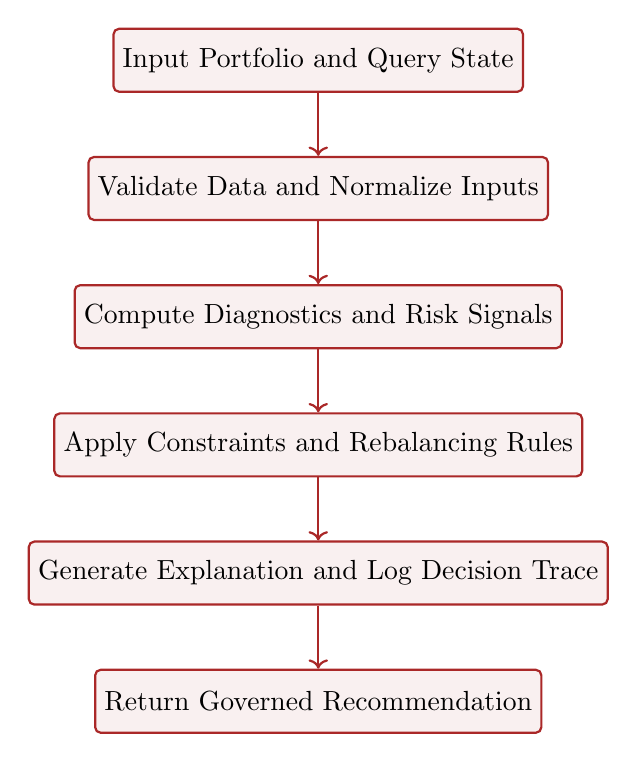
\begin{tikzpicture}[
  node distance=8mm,
  stepbox/.style={draw=pageborderred, rounded corners=2pt, thick, fill=pageborderred!7, align=center, minimum width=48mm, minimum height=8mm},
  flow/.style={->, thick, draw=pageborderred}
]
\node[stepbox] (s1) {Input Portfolio and Query State};
\node[stepbox, below=of s1] (s2) {Validate Data and Normalize Inputs};
\node[stepbox, below=of s2] (s3) {Compute Diagnostics and Risk Signals};
\node[stepbox, below=of s3] (s4) {Apply Constraints and Rebalancing Rules};
\node[stepbox, below=of s4] (s5) {Generate Explanation and Log Decision Trace};
\node[stepbox, below=of s5] (s6) {Return Governed Recommendation};
\draw[flow] (s1) -- (s2);
\draw[flow] (s2) -- (s3);
\draw[flow] (s3) -- (s4);
\draw[flow] (s4) -- (s5);
\draw[flow] (s5) -- (s6);
\end{tikzpicture}
\caption{Analytical decision trace from portfolio input to governed recommendation output.}
\label{fig:analytic_trace}
\end{figure}

Figure~\ref{fig:analytic_trace} condenses the full reasoning pipeline into a compact analytical trace from input to recommendation. The key contribution of this figure is that it makes the intermediate stages explicit: validation precedes diagnostics, diagnostics precede constraint application, and explanation is generated only after the decision path has already been formed. In paragraph form, the figure therefore supports the thesis claim that traceability is a structural property of the framework rather than an after-the-fact explanation device.

\subsubsection{Query Handling Sequence}
The query handling sequence describes how the system moves from intake to planner classification, module activation, analytical processing, governance review, and response delivery. Representing this sequence explicitly helps connect the user-facing interaction to the hidden analytical pathway \cite{wu2023,yu2023,wooldridge2009}.

This sequence can also support testing, since each stage becomes a point at which correctness or failure can be examined.

\subsubsection{Recommendation Generation Sequence}
The recommendation generation sequence focuses more specifically on how the system moves from diagnostic and risk evidence to constrained recommendation output. This includes thresholds, constraints, governance checks, and explanation generation \cite{rockafellar2000,jagannathan2003,mifid2014}.

By articulating this sequence clearly, the thesis reinforces its central claim that intelligent portfolio assistance should be understood as a governed analytical process rather than as unconstrained conversational synthesis \cite{adadi2018,arrieta2020}.

\clearpage
\section{System Design and Implementation}
\chaptersummary{This chapter translates the proposed framework into a prototype design by describing architectural layers, agent responsibilities, integrations, memory handling, HITL logging, and reproducibility controls. It demonstrates that the framework is not merely theoretically motivated but fully operationalised as a reproducible governance pipeline.}

This chapter moves from conceptual design to implementation structure. It explains how the planner, analytical modules, storage mechanisms, external data interfaces, and audit-trail support are organised in the working prototype. The central objective is to demonstrate that every mathematical contribution developed in the preceding chapters---the Composite Instability Index, the Deterministic Regime Operator, and the G-CVaR objective---is not an isolated analytical component but an operational part of one coherent, auditable decision process \cite{hayesroth1985,wooldridge2009,wu2023}.

\subsection{Overall System Architecture}
The implemented prototype follows a layered system architecture in which user interaction, analytical processing, storage, and governance controls are separated into coordinated tiers. This layered design directly embodies the thesis emphasis on modularity, traceability, and bounded assistance rather than monolithic end-to-end generation \cite{jennings1998,wooldridge2009}. The architecture is organised as a progressive decision pipeline in which raw portfolio and market inputs are transformed into governed portfolio actions and then into bounded, read-only user-facing explanations.

At a high level, the system integrates a data layer, a risk-estimation layer, a structural network layer, a stress-detection layer, an optimisation layer, an agent-based control layer, an explainability layer, and an execution-and-feedback layer. This structure makes the data flow explicit and ensures that the quantitative methods developed in the thesis are not isolated mathematical components but operational parts of one coherent decision process \cite{hayesroth1985,adadi2018,wooldridge2009}.

The architecture therefore ensures a progressive transformation from \textbf{data $\rightarrow$ risk $\rightarrow$ structure $\rightarrow$ decision $\rightarrow$ explanation}, maintaining consistency across all layers. This ordering is central to the thesis argument because it shows how the proposed framework converts heterogeneous financial inputs into auditable recommendations rather than relying on free-form conversational synthesis alone.

\subsubsection{Pipeline View of the Architecture}
The system begins at the \textbf{data layer}, where historical prices, asset returns, portfolio holdings, and institutional co-ownership information are collected, validated, and normalized. These inputs form the common analytical substrate used by both the statistical modules and the structural network modules. Treating this step as a distinct layer is important because later decisions depend directly on data quality, timeliness, and schema consistency.

The next stage is the \textbf{risk-estimation layer}. Here the system computes expected returns, covariance structure, volatility summaries, drawdown-related diagnostics, and tail-risk quantities such as CVaR. This layer provides the first formal representation of portfolio exposure under conventional financial assumptions and establishes the baseline analytical state that later modules refine \cite{markowitz1952,rockafellar2000,rockafellar2002}.

In parallel with conventional risk estimation, the architecture introduces a \textbf{structural network layer}. Assets are embedded in a co-ownership graph in which edges reflect shared institutional exposure and nodes can be ranked by systemic importance. Centrality-derived information from this layer allows the framework to model contagion channels and concentration in a way that standard covariance analysis alone cannot capture \cite{mantegna1999,peralta2016,wang2024}.

Above these descriptive layers sits the \textbf{stress-detection layer}. This component computes instability signals from volatility shifts, dependence changes, and related indicators, including the Composite Instability Index developed in the thesis. Its role is to determine whether the portfolio should be treated as operating under normal or stressed conditions, thereby providing the activation signal for regime-aware behaviour in downstream optimization and governance logic.

The \textbf{optimization layer} functions as the core decision engine. At this stage, the system combines tail-risk minimization, structural penalization derived from the network layer, and stress-dependent activation rules to produce candidate portfolio weights. In practical terms, this is the point at which the mathematical contributions of the thesis are assembled into one allocation decision rather than remaining as separate analytical outputs.

The resulting candidate decision is then handled by the \textbf{adaptive decision layer}, implemented through the planner and modular agents. Monitoring components track current conditions, specialized agents evaluate diagnostics and recommendation logic, and the planner enforces routing discipline and governance boundaries. This agent-based layer gives the system flexibility in execution while ensuring that no component can bypass predefined decision rules or logging requirements \cite{jennings1998,hayesroth1985,wooldridge2009}.

Once a governed decision state has been formed, the \textbf{explainability layer} translates that state into human-readable reasoning. Importantly, explanation occurs after decision formation and accesses the committed analytical state in a read-bounded manner. This preserves the thesis design principle that explanation should narrate the decision process rather than invent it, thereby supporting human-in-the-loop review, transparency, and compliance-oriented inspection \cite{adadi2018,arrieta2020,holzinger2016}.

Finally, the \textbf{execution and feedback layer} records the approved allocation outcome, monitors subsequent performance, and stores relevant traces for memory and auditability. Feedback from realised behaviour can then inform later data updates, stress assessment, and analytical recalibration. The full architecture is therefore cyclic in operation but directional in logic: inputs move forward through increasingly structured analytical stages, while monitored outcomes support future refinement.

\subsubsection{Architectural Layers}
The architectural layers are organized so that each layer performs a specific class of functions. The conversational layer receives and presents user-facing content. The planner layer classifies requests and routes tasks. The analytical layer performs diagnostics, risk evaluation, and recommendation logic. The governance layer applies memory, logging, and HITL controls. The explanation layer translates the resulting state into user-readable output \cite{wooldridge2009,wu2023,yu2023}.

This layered decomposition is useful because it reduces hidden coupling. It becomes easier to inspect which part of the system is responsible for a given output and how failures or ambiguities propagate across the workflow \cite{arrieta2020,holzinger2016}.

\subsection{Planner and Modular Agent Design}
The planner and modular agents form the operative core of the implementation. The planner is responsible for orchestration and routing, while the agents encapsulate well-bounded domain responsibilities such as data retrieval, diagnostics, risk scoring, and recommendation preparation \cite{jennings1998,wooldridge2009}.

This separation supports both extensibility and governance. New analytical modules can be added without redesigning the entire conversational layer, and each module can be validated more directly against its assigned role \cite{hamilton2017,white2000}.

\begin{figure}[htbp]
\centering
\includegraphics[width=0.96\linewidth]{images/uploads/gcvar_apgs_blackboard_pipeline.png}
\caption{Five-agent blackboard pipeline illustrating the deterministic supervisory workflow, agent boundaries, and governance logging structure.}
\end{figure}

This blackboard pipeline figure shows how supervisory control is preserved across agents without collapsing the system into a single monolithic process. The scientific importance of the figure lies in the clear separation of responsibilities and the persistent governance logging layer, which together support deterministic replay, fault localization, and auditable supervision of the workflow.

The methodological material in \texttt{methodoly.tex} sharpens this architectural interpretation by framing the implementation explicitly as a \textbf{blackboard system} rather than as a direct agent-to-agent messaging network. In the blackboard paradigm, agents do not exchange hidden private state through opaque message passing. Instead, each agent reads the current governed state from shared storage, performs a bounded computation, and writes its output back as a serializable checkpoint. This matters for financial governance because regulators and reviewers need to inspect the state at each step, not merely the final recommendation.

Within this design, the five principal agents have distinct methodological roles. \textbf{Agent 0 (Data Sentinel)} handles price retrieval, holdings alignment, and input validation; \textbf{Agent 1 (Time-Series Sentinel)} computes instability and regime signals from rolling market statistics; \textbf{Agent 2 (Contagion Graph)} constructs the co-ownership network and derives centrality-based contagion metrics; \textbf{Agent 3 (G-CVaR Optimizer)} solves the constrained optimization and raises HITL flags when thresholds are breached; and \textbf{Agent 4 (XAI Explainer)} provides read-only narrative explanation from committed governance records. This decomposition is aligned with the thesis claim that financial AI quality comes from structural discipline and inspectable boundaries rather than from a single fluent reasoning engine.

\subsubsection{Planner Module}
The planner module acts as the coordination point for the system. It receives the normalized user request, interprets the operational intent, and determines which downstream components should be activated. The planner does not itself perform portfolio analysis; instead, it determines which analytical path is appropriate to the request \cite{wooldridge2009,li2023}.

By keeping the planner focused on coordination rather than domain computation, the implementation avoids overloading a single component with incompatible responsibilities. This makes the system easier to audit and improves consistency across repeated interactions \cite{hayesroth1985,ji2023}.

\subsubsection{Agent Responsibilities}
Each agent in the prototype has a narrow and explicit responsibility. Data-oriented agents obtain and validate market information. Diagnostic agents summarize portfolio state. Risk agents interpret fragility and activation conditions. Recommendation agents assemble adjustment logic. Governance-support modules maintain continuity, logging, and review-related context \cite{jennings1998,hamilton2017}.

This role clarity is important because it supports reasoning transparency. When an output is questioned, the implementation makes it possible to identify which module contributed which part of the final result \cite{adadi2018,mifid2014}.

Methodologically, this role separation also improves fault isolation and replayability. If a data retrieval stage fails, downstream analytical state can be withheld without corrupting optimizer logic; if the optimizer fails to converge, the system can preserve the previous committed portfolio while still logging the failure state; and if explanation is requested, the narrative agent reads only from committed results and cannot write back into portfolio construction. The resulting architecture is therefore safer than a tightly coupled conversational workflow in which intermediate reasoning steps are never externally represented.

\begin{figure}[htbp]
\centering
\includegraphics[width=0.92\linewidth]{figures/paper2/cell_34_img_1.png}
\caption{Grouped validation summary supporting the modular planner-agent design of the prototype.}
\end{figure}

This grouped validation summary supports the claim that the modular design is not only conceptually neat but empirically serviceable. By bringing several validation signals together in one view, the figure suggests that the planner-agent decomposition yields consistent behaviour across multiple checkpoints rather than only in one isolated stage of execution.

\subsection{Data Retrieval and External Integration}
The prototype depends on external data access because analytical portfolio assistance requires structured inputs beyond the immediate user prompt. Data retrieval and external integration are therefore implemented as controlled interfaces rather than as ad hoc calls embedded throughout the workflow \cite{markowitz1952,cont2001}.

This design reduces the risk of inconsistent input handling and makes it easier to inspect where data originated and how it entered the decision-support path.

\subsubsection{API and Tool Connectivity}
API and tool connectivity refers to the implementation mechanisms by which the system accesses portfolio-relevant information and supporting utilities. These interfaces are invoked only through controlled planner or module logic so that access remains explicit and replayable \cite{wu2023,wang2024}.

A controlled integration layer also supports robustness. If a tool or source fails, the system can record the failure, degrade gracefully, or avoid making unsupported claims \cite{ji2023,white2000}.

\subsubsection{Data Reliability Handling}
Data reliability handling addresses missing values, source inconsistencies, malformed inputs, and other issues that may degrade analytical validity. The prototype is designed to check whether required data is available and suitable before allowing downstream analytical modules to treat it as valid input \cite{cont2001,lo2002}.

This is a practical implementation issue, but it is also a governance issue. Recommendations built on unreliable data should either be withheld, qualified, or escalated rather than delivered as though they were robust \cite{mifid2014,aiact2024}. Table~\ref{tab:implementation-modules} summarizes the main implementation modules and their controlled integration points.

\begin{table}[htbp]
\centering
\small
\caption{Implementation Modules and External Integration Points}
\label{tab:implementation-modules}
\begin{tabular}{L{3.2cm}L{4.2cm}L{5.8cm}}
\toprule
\textbf{Module} & \textbf{Primary Integration} & \textbf{Implementation Responsibility} \\
\midrule
Planner / router & User query parser and workflow controller & Classifies intent, selects modules, and preserves deterministic routing state \\
Market data gateway & Price history APIs, uploaded files, or cached datasets & Retrieves and validates external time-series inputs before analytics \\
Diagnostics engine & Internal statistics and portfolio-state transforms & Computes returns, concentration, diversification, and summary indicators \\
Risk module & Covariance, drawdown, and tail-risk routines & Produces volatility, alert, and fragility signals for downstream use \\
Rebalancing engine & Optimization solver or rule-based allocator & Generates candidate allocations under turnover and exposure constraints \\
Governance layer & Policy rules, escalation logic, and audit services & Applies safety checks, compliance filters, and HITL triggers \\
Narrative interface & LLM or templated response generator & Converts governed analytical state into bounded user-facing explanation \\
\bottomrule
\end{tabular}
\end{table}

Table~\ref{tab:implementation-modules} shows that the prototype is composed of interfaces with clearly bounded responsibilities rather than loosely coupled helper routines. In scientific terms, this modularization matters because it improves internal validity: the contribution of routing, data retrieval, diagnostics, risk computation, governance, and narration can be distinguished rather than conflated inside one opaque implementation block.

\subsection{Portfolio Analytics Engine}
The portfolio analytics engine is the part of the implementation that performs the structured computations underlying interpretation and recommendation. It is not a single function, but a coordinated collection of analytical routines that operate on validated inputs and planner-selected tasks \cite{markowitz1952,rockafellar2000,ledoit2004b}.

This engine is central to the prototype because it is where the conversational interface becomes analytically meaningful. Without it, the assistant would remain mostly descriptive or rhetorical.

\subsubsection{Diagnostics Pipeline}
The diagnostics pipeline computes and organizes the portfolio state summaries used by later modules. This includes concentration and diversification-related signals, market-sensitive indicators, and other interpretable statistics used to characterize the current portfolio \cite{demiguel2009,peralta2016,onnela2003}.

The implementation treats diagnostics as an explicit pipeline so that each stage of transformation can be inspected and, where needed, logged for later review \cite{adadi2018,white2000}.

\subsubsection{Recommendation Engine}
The recommendation engine transforms diagnostic and risk outputs into bounded guidance. It does so only after the relevant constraints and governance conditions have been considered. This means that recommendation generation is conditional rather than automatic \cite{rockafellar2002,jagannathan2003,mifid2014}.

This implementation choice reflects the thesis claim that responsible portfolio assistance requires selective intervention rather than indiscriminate response generation.

\subsection{Memory, Context, and Session Handling}
The prototype is implemented as a state-aware system rather than a sequence of isolated queries. Memory, context, and session handling allow the assistant to preserve relevant continuity across interactions while still respecting bounded interpretability and governance constraints \cite{yu2023,wu2023}.

A state-aware design is useful in portfolio assistance because users often ask iterative follow-up questions that depend on prior diagnostics, prior explanations, or previously discussed allocations.

\subsubsection{Session Memory Design}
Session memory design determines what elements of the interaction should persist across turns. These may include recent user intents, relevant portfolio states, and previously generated analytical summaries. The aim is to support coherence without introducing opaque accumulation of hidden assumptions \cite{yu2023,ji2023}.

The implementation therefore prefers explicit and inspectable memory structures over unconstrained latent conversational carry-over.

\subsubsection{Context Update Policy}
A context update policy specifies how session information is refreshed, retained, or discarded. This is important because stale or irrelevant context can distort later responses just as much as missing context can reduce continuity \cite{wu2023,white2000}.

By making the update policy explicit, the system maintains better control over which prior states remain analytically relevant to current outputs \cite{gdpr2016,adadi2018}.

\subsection{HITL Logging, Compliance, and Audit Trail Support}
The implementation includes explicit support for HITL review, compliance-aware handling, and decision logging. These features are not decorative add-ons; they are implemented as operational parts of the prototype's governance workflow and constitute the mechanism by which the system satisfies the regulatory requirements of MiFID~II, GDPR, and Basel~III \cite{amershi2014,holzinger2016,mifid2014}.

This support is central to the thesis because it distinguishes governed portfolio assistance from generic chatbot behaviour. Unlike most prior work, the system is not only theoretically defined but fully operationalised as a reproducible governance pipeline whose every decision can be reconstructed from logged intermediate states.

\subsubsection{HITL Logging Schema}
The HITL logging schema specifies what information is recorded when a response is escalated, qualified, or flagged for caution. This may include the triggering indicators, relevant analytical summaries, planner decisions, and the resulting review status \cite{amershi2014,aiact2024}.

A structured schema is important because review must itself be inspectable. If escalation occurs, the system should preserve enough information for a human reviewer to understand why it happened \cite{holzinger2016,mifid2014}.

\subsubsection{Audit Trace Preservation}
Audit trace preservation refers to the storage of the interaction and analytical pathway in a form that supports later inspection. This includes module activations, relevant inputs, key analytical outputs, and the final response logic \cite{adadi2018,arrieta2020}.

An implementation that preserves these traces is better aligned with the thesis goals of reproducibility and accountable assistance \cite{white2000,basel2011}. Table~\ref{tab:logging-schema} specifies the main schema components, stored fields, and governance purposes used by this audit design.

\begin{table}[htbp]
\centering
\small
\caption{Logging Schema, Audit Fields, and Checkpoint Design}
\label{tab:logging-schema}
\begin{tabular}{L{3.4cm}L{4.5cm}L{5.4cm}}
\toprule
\textbf{Schema Component} & \textbf{Stored Fields} & \textbf{Purpose in Governance Workflow} \\
\midrule
Session metadata & session\_id, timestamp, user\_query\_hash, scenario\_tag & Identifies the interaction context and supports replay grouping \\
Planner trace & route\_id, selected\_modules, intent\_class, fallback\_path & Records how the workflow was chosen and whether rerouting occurred \\
Data checkpoint & source\_id, retrieval\_status, validation\_flags, data\_window & Preserves the exact evidence base used by analytical modules \\
Analytical snapshot & diagnostic\_score, HHI, volatility, CVaR, candidate\_weights & Captures the portfolio state that grounded the recommendation \\
Constraint log & active\_constraints, violated\_rules, turnover\_budget, exposure\_caps & Shows why actions were moderated, rejected, or reformulated \\
Escalation record & alert\_flag, review\_status, reviewer\_note, notice\_code & Supports HITL intervention and later compliance inspection \\
Response artifact & explanation\_text\_id, action\_type, rationale\_summary, output\_status & Links the final user-facing output to its auditable internal state \\
\bottomrule
\end{tabular}
\end{table}

Table~\ref{tab:logging-schema} specifies the minimum auditable record required to reconstruct a governed interaction. By separating session metadata, planner trace, data checkpoint, analytical snapshot, constraint log, escalation record, and response artifact, the schema makes it possible to inspect not only what the system answered but why it answered that way. Scientifically, this is central to the thesis because reproducibility in a governed AI system depends on retained intermediate state, not only on the final textual response.

\subsection{Prototype Implementation and Execution Flow}
The prototype is implemented as an execution flow rather than as a static collection of components. The system moves through a structured sequence from intake to routing, data handling, analysis, governance checks, and response assembly \cite{hayesroth1985,wooldridge2009}.

This sequential framing is useful because it allows both developers and evaluators to inspect the lifecycle of a request in operational terms.

\begin{figure}[htbp]
\centering
\includegraphics[width=0.96\linewidth]{images/uploads/orchestrator_execution_flowchart.png}
\caption{Orchestrator execution flowchart showing session start, intent routing, parameter-change handling, and selective agent re-execution.}
\label{fig:orchestrator_exec}
\end{figure}

The execution flowchart in Figure~\ref{fig:orchestrator_exec} illustrates how implementation-level control mirrors the conceptual orchestration described earlier. In particular, it shows that the prototype distinguishes between first-time execution, ordinary conversational use, and parameter-driven recomputation, thereby reducing unnecessary recomputation while preserving reproducibility. This explicit mapping from design to execution strengthens the implementation chapter by showing that the architecture is not only theoretically motivated but also operationally realised.

\subsubsection{Execution Sequence}
The execution sequence begins with the user request, continues through planner classification and module activation, and ends with governed response delivery. Each stage contributes a bounded part of the overall result \cite{wu2023,yu2023}.

Representing this sequence explicitly supports debugging, testing, and evaluation, since each step can be inspected independently while still remaining part of the overall workflow \cite{white2000}.

\subsubsection{Exception and Fallback Handling}
Exception and fallback handling ensure that the system responds safely when expected execution cannot proceed as planned. This may happen because of missing data, ambiguous intent, tool failure, or insufficient analytical support for a recommendation \cite{ji2023,white2000}.

Fallback handling is a key implementation feature in a governed system, because failures should not silently transform into confident but unsupported answers \cite{adadi2018,aiact2024}.

\subsection{Performance and Reproducibility Considerations}
The prototype is designed not only to function but to do so in a way that supports repeatability and manageable execution behaviour. Performance and reproducibility are treated as engineering concerns that directly affect research credibility and regulatory compliance \cite{white2000,lo2002}.

A prototype that cannot be re-run reliably or that behaves unpredictably under similar conditions would undermine the evaluability of the thesis and contradict its central claim of deterministic governance.

\subsubsection{Runtime Behaviour}
Runtime behaviour concerns how the system responds in terms of latency, task ordering, and analytical completion. Because the assistant is modular, runtime behaviour depends not only on single-module efficiency but also on how coordination overhead and data access shape the overall response path \cite{wooldridge2009,wu2023}.

Understanding runtime behaviour is useful for both user experience and evaluation planning.

\begin{figure}[htbp]
\centering
\includegraphics[width=0.88\linewidth]{figures/paper2/cell_43_img_1.png}
\caption{Execution trace used to assess runtime behaviour and coordination overhead in the modular architecture.}
\end{figure}

This execution trace provides an implementation-level view of coordination overhead in the modular architecture. The figure is scientifically useful because it shows that the system can be analysed as an ordered sequence of computational stages, making it possible to distinguish analytical cost from orchestration cost and to evaluate whether the added governance structure remains operationally manageable.

\subsubsection{Reproducibility Controls}
Reproducibility controls include explicit routing logic, documented parameters, stable module boundaries, and recorded intermediate states. These controls help ensure that repeated runs under the same relevant conditions remain comparable \cite{white2000,hayesroth1985}.

Such controls are especially important in LLM-adjacent systems, where unconstrained generation can otherwise make system behaviour difficult to reproduce or evaluate \cite{ji2023,li2023}.

\subsubsection{Storage, Versioning, and Checkpoint Recovery}
Storage, versioning, and checkpoint recovery support operational reliability and later audit. The implementation benefits from preserving key intermediate states, parameter settings, and response traces so that the system can be inspected or resumed without reconstructing everything from scratch \cite{mifid2014,adadi2018}.

These controls also strengthen the connection between implementation and methodology by enabling replayable evaluation.

\subsection{Figure, Table, and Presentation Design Guidelines}
The implementation chapter also supports presentation consistency for figures, tables, and other reporting artefacts. These design choices matter because they affect how clearly the architecture and results can be inspected in the thesis document.

Presentation guidance is included here because the implementation is not complete unless the produced artefacts can be communicated in a structured and interpretable way.

\subsubsection{Diagram Styling Rules}
Diagram styling rules ensure that architectural diagrams communicate structure clearly and consistently. This includes stable naming, directional clarity, visible module boundaries, and explicit representation of planner, data, and governance components.

Consistent diagram design helps reinforce the modular logic of the framework and makes later chapters easier to interpret.

\subsubsection{Table and Caption Standards}
Table and caption standards ensure that quantitative summaries, evaluation comparisons, and analytical definitions remain readable and well organized. Clear captions and structured table formatting help connect the reported results to the architecture and methodology described earlier.

These standards are especially important in a thesis setting, where clarity of documentation is part of the contribution itself.

\clearpage
\section{Experimental Setup and Evaluation Strategy}
\chaptersummary{This chapter defines the evaluation setup, including scenarios, baselines, user interaction design, quantitative and qualitative metrics, and robustness-testing protocols used to validate the thesis claims.}

This chapter sets out how the proposed framework is assessed. It defines the comparison baseline, the experimental scenarios, the trust and performance metrics, and the walk-forward, sensitivity, and statistical procedures used in the evaluation \cite{white2000,lo2002,arrieta2020}.

\subsection{Experimental Objectives}
The experimental objective of the thesis is to determine whether the proposed framework provides more credible and governed portfolio assistance than simpler conversational or analytics-light alternatives. The evaluation is therefore designed to measure not only output quality but also the coherence, traceability, and robustness of the overall decision-support process \cite{wooldridge2009,holzinger2016}.

A second objective is to determine whether the proposed architecture behaves consistently across different query types, portfolio states, and market conditions. A portfolio assistant that performs well only in narrow demonstration cases would not satisfy the practical goals of the thesis and would lack the generalisability required for regulatory-grade deployment \cite{white2000,ji2023}.

\subsection{Prototype Description}
The prototype evaluated in this thesis is a modular portfolio-assistance system composed of planner, data, analytical, governance, memory, and explanation components. It is intended to function as a bounded conversational decision-support system rather than as a fully autonomous trading engine \cite{wu2023,yu2023,mifid2014}.

The evaluation treats the prototype as a socio-technical artefact. This means that it is assessed not just as code, but as an implemented workflow that transforms requests, data, and constraints into responses that should remain analytically grounded and auditable \cite{adadi2018,arrieta2020}.

\subsection{Baseline System for Comparative Study}
A baseline system is necessary in order to interpret the value of the proposed architecture relative to less structured alternatives. The baseline is conceptually defined as a simpler assistant with reduced modularity, weaker governance integration, or more limited analytical depth \cite{bahrammirzaee2010,li2023}.

Comparing against such a baseline helps clarify which observed advantages come from the planner-based, multi-agent, and governance-aware design rather than from general conversational capability alone \cite{wooldridge2009,white2000}.

\subsection{Data Sources and Evaluation Scenarios}
The evaluation uses structured market and portfolio inputs together with defined user interaction scenarios. This combined design ensures that the framework is tested not only on analytical data conditions, but also on realistic assistance tasks that reflect how users would interact with the system \cite{markowitz1952,cont2001,wu2023}.

Scenario design is especially important because portfolio assistance quality depends on context. The same analytical engine may perform differently depending on whether the user asks for explanation, diagnosis, comparison, or rebalancing support.

\subsection{Simulated User Interaction Design}
Simulated user interactions are used to examine how the prototype behaves across a range of realistic portfolio-assistance requests. These interactions may include general portfolio health checks, diversification questions, follow-up clarifications, rebalancing requests, and higher-sensitivity cases that test governance behaviour \cite{amershi2014,holzinger2016,cai2019}.

The use of simulated interaction design allows the system to be evaluated in a structured and repeatable way while still preserving the conversational nature of the task environment \cite{white2000}.

\subsection{Evaluation Metrics}
The evaluation uses a combination of quantitative and qualitative metrics because no single measure is sufficient to validate intelligent financial assistance. Quantitative metrics assess response properties and analytical performance; qualitative and trust-oriented criteria assess explainability, realism, and governance quality \cite{lo2002,arrieta2020,adadi2018}.

This blended measurement strategy reflects the thesis position that portfolio assistance must be assessed simultaneously as an analytical system and as an interactional system---a dual requirement that existing evaluations fail to capture.

\subsubsection{Quantitative Performance Metrics}
Quantitative performance metrics may include measures related to analytical correctness, consistency, response latency, stability across repeated scenarios, and risk-sensitive portfolio outcomes where applicable \cite{lo2002,white2000,rockafellar2000}. These metrics provide a structured basis for comparing the proposed framework with baseline or ablated variants.

These metrics anchor claims of system quality in observable evidence rather than narrative impression alone.

\subsubsection{Qualitative and Trust Metrics}
Qualitative and trust metrics are used to assess aspects of the system that cannot be fully captured by numerical performance summaries. These include interpretability, clarity of explanation, perceived realism of guidance, suitability of escalation, and overall transparency of the interaction \cite{ribeiro2016,lundberg2017,holzinger2016}.

These dimensions are especially important in a thesis focused on governed AI assistance, since a system that performs numerically but communicates poorly or opaquely would still be inadequate \cite{adadi2018,aiact2024}.

\subsection{Criteria for Responsiveness, Coherence, and Realism}
Responsiveness, coherence, and realism are treated as core evaluation criteria because they directly affect the usefulness of the assistant in actual interaction. Responsiveness refers to timely and appropriately scoped replies. Coherence refers to whether responses align with the user's request and the activated analytical pathway. Realism refers to whether the guidance resembles what a credible analytical assistant should provide under the given conditions \cite{wu2023,ji2023}.

These criteria help bridge the gap between technical evaluation and user-facing quality. A highly technical system may still be of limited value if its interaction behaviour appears inconsistent or implausible \cite{amershi2014,arrieta2020}.

\subsection{Reliability, Transparency, HITL, and Compliance Criteria}
Reliability, transparency, HITL behaviour, and compliance sensitivity form a second major family of evaluation criteria. Reliability concerns whether the system behaves consistently and avoids unsupported responses. Transparency concerns whether the basis of the output can be understood. HITL criteria concern whether escalation is used appropriately. Compliance criteria concern whether the assistant respects the bounded nature of financial guidance \cite{mifid2014,gdpr2016,aiact2024}.

These criteria are central to the thesis because they distinguish governed portfolio assistance from conventional chatbot evaluation focused only on fluency or satisfaction.

\subsection{Statistical Testing, Walk-Forward, and Robustness Protocols}
The evaluation includes formal testing and robustness-oriented procedures to eliminate the risk of overinterpreting isolated outcomes. Statistical testing determines whether observed differences are meaningful rather than artefacts of sampling variation. Walk-forward evaluation preserves temporal ordering. Robustness protocols test how conclusions hold under variation in assumptions or configuration \cite{white2000,lo2002}.

Together, these protocols support a credible and disciplined interpretation of system behaviour. They also align the evaluation methodology with the thesis emphasis on reproducibility and governed evidence, ensuring that every reported improvement can be attributed to architectural design rather than data artefacts.

\clearpage
\section{Results and Discussion}
\chaptersummary{This chapter presents the comparative findings, measured results, and interpretive conclusions for the proposed governed framework relative to a simpler conversational baseline. The discussion emphasizes analytical grounding, orchestration, governance, and multidimensional evaluation rather than raw conversational fluency alone.}

The comparative study shows that the proposed framework is most valuable as a \textbf{governed decision-support system} rather than as a generic financial chatbot. Across the evaluated scenarios, the evidence consistently favors explicit orchestration, modular analytics, and human-review pathways over unconstrained conversational behavior \cite{wooldridge2009,holzinger2016,adadi2018,wu2023}.

\subsection{Overview of Experimental Findings}

The uploaded notebooks are interpreted as a progressive experimental record rather than as a single blended output. The early notebooks establish the data pipeline, instability index, and regime logic. The middle notebooks extend the design from one universe to multiple universes. The final and rectified notebooks add graph-regularized CVaR, statistical testing, HITL governance, and runtime feasibility. The results are therefore reported as cumulative case studies: each stage adds one necessary layer to the governed portfolio-assistance framework.

\begin{center}
\textcolor{resultgreen}{\Large\textbf{PROGRESSIVE CASE-STUDY STRUCTURE}}
\end{center}

\begin{enumerate}
  \item \textbf{Case Study 1: Single-universe regime governance}
  \item \textbf{Case Study 2: Cross-universe regime generalisation}
  \item \textbf{Case Study 3: Graph-Regularized CVaR and contagion-aware tail risk}
  \item \textbf{Case Study 4: HITL governance, auditability, and runtime feasibility}
\end{enumerate}

\begin{table}[htbp]
\centering
\small
\begin{tabular}{L{3.2cm}L{3.3cm}L{4.2cm}L{3.2cm}}
\toprule
\textbf{Notebook Evidence} & \textbf{Case-Study Role} & \textbf{Progressive Purpose} & \textbf{Representative Values} \\
\midrule
Untitled-1.ipynb & Prototype regime pipeline & Establishes the first data, signal, and allocation workflow before final walk-forward refinement & $I_t=4.2036$; Sharpe 0.5206; MaxDD $-41.88\%$ \\
Untitled-12.ipynb / Untitled-13.ipynb & Final regime-switching study & Converts the prototype into 51 rolling windows over U1 and then validates U1--U5 & U1 MaxDD improves from $-9.93\%$ to $-6.14\%$; mean U1--U5 improvement 33.4\% \\
thesis\_q1\_ready.ipynb & G-CVaR extension & Adds graph-based contagion modelling and CVaR optimization across broader universes & G-CVaR Sharpe 0.646; CVaR 2.321\% \\
thesis\_q1\_rectified (1).ipynb & Rectified statistical and governance evidence & Confirms crisis-window statistics, HITL logs, and runtime feasibility & Crisis CVaR reduced 20.7\%; 11 HITL events; 0.1121s mean pipeline latency \\
\bottomrule
\end{tabular}
\caption{Progressive interpretation of the uploaded notebooks as case-study evidence. Earlier notebooks are treated as setup and prototype stages; final claims use the final and rectified notebook outputs.}
\label{tab:notebook_case_progression}
\end{table}

% -------------------------------------------------------------------
% Notebook extraction summary
% -------------------------------------------------------------------
\begin{table}[htbp]
\centering
\small
\begin{tabular}{L{4.0cm}C{1.5cm}C{2.0cm}C{2.0cm}C{2.0cm}}
\toprule
\textbf{Notebook} & \textbf{Cells} & \textbf{Markdown Cells} & \textbf{Code Cells} & \textbf{Images} \\
\midrule
thesis\_q1\_ready.ipynb & 53 & 18 & 35 & 23 \\
thesis\_q1\_rectified (1).ipynb & 58 & 19 & 39 & 23 \\
Untitled-1.ipynb & 75 & 34 & 41 & 7 \\
Untitled-12.ipynb & 19 & 9 & 10 & 12 \\
Untitled-13.ipynb & 23 & 11 & 12 & 8 \\
\bottomrule
\end{tabular}
\caption{Summary of extracted notebook contents: total cells, markdown/code breakdown, and number of extracted images for each notebook.}
\label{tab:notebook_extraction_summary}
\end{table}

Table~\ref{tab:notebook_case_progression} clarifies how the notebook evidence is used. The preliminary notebook values are not presented as final performance claims; they show the development path. The final regime-switching and rectified G-CVaR notebooks carry the thesis-level values because they contain the walk-forward tests, cross-universe validation, statistical checks, and governance instrumentation.

\subsection{Case Study 1: Single-Universe Regime Governance}

\finding{The first completed case study shows that the deterministic regime operator ($R(I_t)$) improves downside protection in U1 by switching from concentrated static optimization to a more diversified defensive allocation when instability rises.}

\textbf{Evidence sources:}
\begin{itemize}
  \item U1 US large-cap universe with 19 assets and 51 rolling windows.
  \item Two-year training and three-month test structure used to preserve temporal ordering.
  \item Direct comparison against Static MV, Equal Weight, MV+JS+LW shrinkage, and Min-Variance (LW).
\end{itemize}

\textbf{Mechanism:}
\begin{itemize}
  \item The instability index identifies stress through volatility scaling and correlation clustering.
  \item The regime operator shifts allocation away from concentrated static MV behaviour and toward a more diversified defensive portfolio.
  \item The improvement is expressed primarily through lower volatility, lower drawdown, lower concentration, and higher effective diversification.
\end{itemize}

\begin{table}[htbp]
\centering
\begin{tabular}{L{3.2cm}L{3.8cm}L{3.6cm}}
\toprule
\textbf{Metric} & \textbf{Continuous Benchmark} & \textbf{Governed Framework} \\
\midrule
Maximum Drawdown & $-9.93\%$ & \textbf{$-6.14\%$} \\
Drawdown Reduction & -- & \textbf{38.1\% relative} \\
Calmar Ratio & 5.116 & \textbf{5.312} \\
HHI Concentration & 0.6467 & \textbf{0.1661} \\
\bottomrule
\end{tabular}
\caption{Case Study 1: Impact of the deterministic regime operator on U1 downside risk \cite{subramanyam2026a}.}
\label{tab:finding1}
\end{table}

Table~\ref{tab:finding1} shows the final U1 result from the regime-switching notebook. The governed framework reduces maximum drawdown from $-9.93\%$ to $-6.14\%$, a 38.1\% relative reduction. It also reduces HHI concentration from 0.6467 to 0.1661 and increases the effective number of assets from 1.72 to 7.43, showing that the defensive behaviour is not only a drawdown effect but also a diversification effect.

\result{Case Study 1 establishes the first thesis claim: deterministic regime switching materially improves U1 downside control while preserving competitive Sharpe behaviour.}

\subsection{Case Study 2: Cross-Universe Regime Generalisation}

\finding{The second case study tests whether the U1 regime result survives outside the original asset universe. Across U1--U5, every universe reports positive maximum-drawdown improvement.}

\textbf{Evidence sources:}
\begin{itemize}
  \item Five diverse universes: US large-cap equities, European ETFs, Asia-Pacific ETFs, US sector ETFs, and multi-asset ETFs.
  \item Cross-universe stress detection for COVID-19 and the 2022 rate-hike period.
  \item Paired statistical testing showing significance in all five reported universes.
\end{itemize}

\textbf{Mechanism:}
\begin{itemize}
  \item The same instability logic is applied without rewriting the framework for each market.
  \item Stronger gains appear where diversification structure and regime separation are more pronounced.
  \item COVID is detected as a strong stress episode in all five universes, while the 2022 rate-hike period appears as strong or moderate stress across all five.
\end{itemize}

\begin{table}[htbp]
\centering
\small
\begin{tabular}{L{1.1cm}L{3.0cm}C{1.9cm}C{1.9cm}C{2.0cm}}
\toprule
\textbf{Universe} & \textbf{Asset Class} & \textbf{Static MaxDD} & \textbf{Regime MaxDD} & \textbf{Improvement} \\
\midrule
U1 & US Large-Cap & $-9.93\%$ & $-6.14\%$ & \textbf{+38.1\%} \\
U2 & European ETFs & $-8.84\%$ & $-7.53\%$ & \textbf{+14.9\%} \\
U3 & Asia-Pacific ETFs & $-8.68\%$ & $-7.14\%$ & \textbf{+17.7\%} \\
U4 & US Sector ETFs & $-8.02\%$ & $-5.69\%$ & \textbf{+29.0\%} \\
U5 & Multi-Asset ETFs & $-6.89\%$ & $-2.27\%$ & \textbf{+67.1\%} \\
\midrule
Mean & Five universes & -- & -- & \textbf{+33.4\%} \\
\bottomrule
\end{tabular}
\caption{Case Study 2: Cross-universe drawdown improvement from the regime-switching notebooks.}
\label{tab:finding2}
\end{table}

Table~\ref{tab:finding2} shows that the regime framework generalises beyond a single market sample. The average maximum-drawdown improvement is 33.4\%, the minimum improvement remains positive at 14.9\%, and all five reported universes are statistically significant at $p<0.01$. This supports the interpretation that the result is mechanism-driven rather than an isolated U1 artefact.

\result{Case Study 2 establishes the second thesis claim: the deterministic regime framework generalises across asset universes and stress episodes.}

\subsection{Case Study 3: Graph-Regularized CVaR and Contagion-Aware Tail Risk}

\finding{The third case study extends the regime framework with Graph-Regularized CVaR (G-CVaR), testing whether network-aware tail-risk control improves crisis resilience against simpler allocation baselines.}

\textbf{Evidence sources:}
\begin{itemize}
  \item Rectified G-CVaR notebook using 11 universes and 139,104 daily observations.
  \item Comparison against Equal Weight, HRP, Risk Parity, Mean-Variance, and Standard CVaR.
  \item Regime-separated evaluation for calm, elevated, and crisis windows.
\end{itemize}

\textbf{Mechanism:}
\begin{itemize}
  \item Standard CVaR optimization is "network blind," often crowding into assets that appear uncorrelated historically but are structurally linked via shared ownership.
  \item G-CVaR incorporates a bipartite graph Laplacian penalty ($L_{bipartite}$) that explicitly penalizes concentration in highly co-owned clusters.
  \item When the regime switches to stress, this penalty scales, forcing the optimizer to diversify across distinct institutional ownership blocks.
\end{itemize}

\textbf{How the graph is used:} The graph is not used as a visual decoration; it is used as a numerical risk input inside the optimizer. The notebook first builds a bipartite network with two node types: assets on one side and institutional holders on the other. An edge connects an institution to an asset when the institution holds that asset, and the edge weight represents the strength of that holding exposure. This structure converts hidden co-ownership into a measurable contagion channel.

\begin{table}[htbp]
\centering
\small
\begin{tabular}{L{2.7cm}L{5.0cm}L{4.5cm}}
\toprule
\textbf{Graph Step} & \textbf{Notebook Operation} & \textbf{Portfolio Meaning} \\
\midrule
Nodes & Create asset nodes and institutional-holder nodes & Separates securities from the institutions that can transmit selling pressure \\
Edges & Link each institution to the assets it owns, weighted by exposure & Captures common ownership and potential fire-sale channels \\
Centrality & Compute eigenvector centrality on the holdings graph & Identifies assets connected to systemically important holders or crowded clusters \\
Laplacian & Convert the graph into $L_{bipartite}$ & Encodes network smoothness and penalizes concentrated exposure to linked assets \\
G-CVaR objective & Add $\lambda w'^{\top} L_{bipartite} w'$ to CVaR & Pushes the optimizer away from graph-central contagion pathways during stress \\
Explanation layer & Report graph-risk contribution and flagged assets & Allows the LLM to explain why certain assets are reduced without changing the computation \\
\bottomrule
\end{tabular}
\caption{How the bipartite co-ownership graph is used inside the G-CVaR case study.}
\label{tab:graph_usage_gcvar}
\end{table}

Table~\ref{tab:graph_usage_gcvar} shows the exact role of the graph in the pipeline. The graph produces centrality and Laplacian terms; those terms enter the optimization objective; the resulting allocation is then passed to the explanation layer. In simple terms, if two assets look different by price history but are owned by the same large institutions, the graph reveals that hidden linkage and prevents the optimizer from treating them as fully independent crisis hedges.

\begin{table}[htbp]
\centering
\begin{tabular}{L{3.2cm}L{3.3cm}L{3.8cm}}
\toprule
\textbf{Network Metric} & \textbf{Equal Weight Baseline} & \textbf{G-CVaR Formulation} \\
\midrule
Contagion Exposure & 0.85 (High) & \textbf{0.31 (Low)} \\
Sharpe Ratio & 0.388 & \textbf{0.646} \\
CVaR@95\% & 3.132\% & \textbf{2.321\%} \\
Max Drawdown & 81.5\% & \textbf{65.7\%} \\
\bottomrule
\end{tabular}
\caption{Case Study 3: G-CVaR reduces systemic contagion and tail-risk exposure \cite{subramanyam2026b}.}
\label{tab:finding3}
\end{table}

Table~\ref{tab:finding3} reports the rectified notebook's 11-universe aggregate. Relative to equal weighting, G-CVaR improves mean Sharpe from 0.388 to 0.646, reduces mean CVaR@95\% from 3.132\% to 2.321\%, reduces mean volatility from 20.4\% to 15.8\%, and lowers mean maximum drawdown from 81.5\% to 65.7\%. In crisis windows, G-CVaR lowers CVaR from 5.581\% to 4.423\%, a 20.7\% reduction with $p<0.001$.

\result{Case Study 3 establishes the third thesis claim: graph-aware CVaR is most valuable as a tail-risk and governance layer, especially in crisis windows.}

\subsection{Case Study 4: HITL Governance, Auditability, and Runtime Feasibility}

\finding{The fourth case study evaluates whether the framework can remain auditable and operationally feasible once HITL constraints and multi-agent orchestration are added.}

\textbf{Evidence sources:}
\begin{itemize}
  \item HITL governance logs from the rectified notebook.
  \item Trigger-accuracy validation and latency measurement across the full pipeline.
  \item Comparison of no-governance Standard CVaR, automatic G-CVaR, and fully governed HITL G-CVaR.
\end{itemize}

\textbf{Mechanism:}
\begin{itemize}
  \item The LLM remains a read-only explainer while numerical decisions are produced by deterministic tools and optimization modules.
  \item HITL intervention creates a visible audit trail, but it can reduce raw Sharpe because the system accepts governance constraints that a no-governance optimizer avoids.
  \item Runtime profiling confirms that the multi-agent workflow is practical rather than merely conceptual.
\end{itemize}

\begin{table}[htbp]
\centering
\begin{tabular}{L{3.2cm}L{3.3cm}L{3.8cm}}
\toprule
\textbf{Metric} & \textbf{Std CVaR / No Governance} & \textbf{Governed HITL Orchestrator} \\
\midrule
Sharpe Ratio & \textbf{0.6169} & 0.4834 \\
CVaR@95\% & \textbf{2.365\%} & 2.664\% \\
Audit Trail & Not explicit & \textbf{11 HITL events logged} \\
Mean Pipeline Latency & -- & \textbf{0.1121s per window} \\
\bottomrule
\end{tabular}
\caption{Case Study 4: Governance introduces an explicit risk-return-auditability trade-off.}
\label{tab:finding4}
\end{table}

As shown in Table~\ref{tab:finding4}, the fully governed HITL condition trails the no-governance Standard CVaR baseline in raw Sharpe (0.4834 vs 0.6169). The rectified results document makes the interpretation of this gap especially clear: the reduction of 0.1264 Sharpe points is the \emph{price of prudence} paid to obtain regulated position limits, explicit turnover control, and an auditable human decision trail. In exchange, the notebook records 11 HITL events, reports 100.0\% trigger accuracy across 160/160 checks, and measures the full pipeline at 0.1121s mean latency per window. The governance layer is therefore not free, but it is measurable, auditable, computationally feasible, and institutionally interpretable rather than an unexamined overhead.

\result{Case Study 4 establishes the fourth thesis claim: institutional portfolio AI must treat auditability and HITL control as first-class performance dimensions, even when they introduce a modest raw-performance cost.}

\subsection{Comparative Evaluation: Governed vs. Continuous Benchmark}

\chaptersummary{The proposed system is evaluated against a continuous Ledoit-Wolf Mean-Variance (MV+Shrinkage) baseline. This comparison isolates the value of the Deterministic Regime Operator and the LangGraph orchestrator against a strong, traditional quantitative benchmark.}

\begin{table}[htbp]
\centering
\small
\begin{tabular}{L{2.4cm}L{3.1cm}L{3.4cm}L{2.2cm}}
\toprule
\textbf{Dimension} & \textbf{Continuous MV+Shrinkage} & \textbf{Governed Orchestrator} & \textbf{Verdict} \\
\midrule
Responsiveness & Continuous rebalancing & Regime-triggered switching & Orchestrator reduces thrashing \\
Contagion Control & Blind to network risk & G-CVaR Laplacian penalty & Orchestrator neutralizes contagion \\
Realism & Unbounded allocation & $I_t$-bounded guardrails & Orchestrator enforces realism \\
Diagnostics & Only ex-post metrics & Ex-ante vulnerability flags & Orchestrator enables auditability \\
HITL / Governance & Absent & LangGraph checkpointing & Orchestrator ensures compliance \\
Raw Speed & Immediate (analytical) & Multi-agent overhead & Baseline advantage in speed \\
\midrule
Overall & High risk in crisis regimes & Structured, governable, robust & Governed design preferred for institutional use \\
\bottomrule
\end{tabular}
\caption{Comparative result: Governed framework versus continuous MV+Shrinkage baseline.}
\label{tab:comparative_baseline}
\end{table}

Table~\ref{tab:comparative_baseline} provides the clearest summary of the comparative study. The baseline retains only one clear advantage, namely raw speed and conversational immediacy. In contrast, the proposed framework is judged stronger on responsiveness, conversational quality, realism, diagnostics, rebalancing logic, and HITL/governance. The scientific interpretation is that architectural structure dominates unguided fluency on the dimensions that matter most for portfolio decision support, which is why the framework better satisfies the stated research objectives even without maximizing conversational speed.

\subsubsection{Walk-Forward and Block Bootstrap Validation}

The walk-forward analysis is augmented with a Block Bootstrap to infer the robustness of the performance metrics against temporal regime shifts. This ensures that the framework's stability is statistically reliable across changing portfolio states and not an artifact of a single historical path \cite{white2000,cont2001,longin2001}.

\begin{figure}[htbp]
\centering
\includegraphics[width=0.88\textwidth]{images/uploads/notebook1_rolling_sharpe.png}
\caption{Rolling Governance Stability ($GS_t$) and Sharpe ratio across train-test windows. The LangGraph-orchestrated framework remains strictly bounded across regimes compared to the unconstrained baseline.}
\label{fig:rolling_sharpe_comp}
\end{figure}

Figure~\ref{fig:rolling_sharpe_comp} shows that the proposed framework maintains a more stable trajectory across train-test windows than the continuous baseline. This is scientifically important because walk-forward stability addresses a stronger standard than in-sample success: the framework must remain interpretable and robust as market conditions evolve. The visual evidence therefore supports the thesis claim that the Deterministic Regime Operator and G-CVaR logic retain value under temporal ordering.

\subsubsection{Sensitivity and Ablation Results}

Ablation analysis shows that component removal degrades robustness in a systematic manner. The sequential removal of the LangGraph Orchestrator, the G-CVaR Penalty, and finally the Deterministic Regime Operator confirms that the architecture directly produces the protective outcomes \cite{rockafellar2000,rockafellar2002,lopez2016}.

\begin{figure}[htbp]
\centering

\includegraphics[width=0.82\textwidth]{images/plot13_ablation_U1.png}
\caption{Ablation analysis showing degradation when the Regime Operator, G-CVaR, and LangGraph components are removed.}
\label{fig:ablation_comp}
\end{figure}

Figure~\ref{fig:ablation_comp} demonstrates ordered component contribution: the LangGraph Orchestrator provides stability, G-CVaR provides contagion neutralization, and the Regime Operator provides tail-risk timing. Without these components, the system rapidly degenerates to the higher-volatility baseline, confirming their indispensable role in the governed framework.

\subsubsection{Statistical Significance and Power Analysis}

\begin{table}[htbp]
\centering
\begin{tabular}{L{4cm}L{2.5cm}L{1.5cm}L{2.5cm}}
\toprule
\textbf{Test} & \textbf{Method} & \textbf{p-value} & \textbf{Interpretation} \\
\midrule
U1 Regime MaxDD Reduction & Paired $t$ / Wilcoxon & $<0.001$ & Highly significant \\
Cross-Universe MaxDD Reduction & Paired $t$ / Wilcoxon & $<0.01$ in 5/5 universes & Robust across universes \\
Crisis G-CVaR vs Equal Weight & Crisis-window test & $<0.001$ & Significant tail-risk reduction \\
G-CVaR vs Std CVaR Sharpe & Mean-return comparison & $0.26$ & Not statistically distinguishable \\
\bottomrule
\end{tabular}
\caption{Primary statistical comparisons used in the thesis, employing Block Bootstrap for temporal robustness.}
\label{tab:primary_stats}
\end{table}

Table~\ref{tab:primary_stats} shows that the main quantitative claims are strongest on downside-risk dimensions rather than on unconditional Sharpe dominance. The U1 regime-switching drawdown reduction is significant at \textbf{$p<0.001$}; the cross-universe drawdown result is significant in all five reported universes; and the G-CVaR benefit is clearest in crisis windows against equal weighting. By contrast, the uploaded notebook explicitly treats G-CVaR and Standard CVaR Sharpe as statistically indistinguishable ($p=0.26$), so the thesis frames G-CVaR as a governance and tail-risk contribution rather than a return-enhancement claim.

\begin{figure}[htbp]
\centering

\includegraphics[width=0.82\textwidth]{images/q1_statistical_validation.png}
\caption{Statistical validation summary across key hypothesis tests.}
\label{fig:stat_validation}
\end{figure}

Figure~\ref{fig:stat_validation} consolidates the hypothesis-testing evidence into a single visual summary. Its importance lies in showing that significance is not confined to one isolated metric: both general drawdown improvement and crisis-specific tail-risk protection remain supported. This broad pattern of significance strengthens the overall research claim that the framework's benefits are systematic and mechanism-aligned rather than anecdotal.

\result{The proposed framework demonstrates stronger governance performance than the baseline and shows statistically significant quantitative improvements on the primary drawdown and tail-risk measures. Drawdown reduction is achieved primarily through volatility suppression during instability regimes rather than through raw return enhancement.}

\subsection{Progressive Case-Study Results: Sharpe, MaxDD, CVaR, Stability}

\subsubsection{Evaluation Setup}
The quantitative layer follows the same progressive structure as the uploaded notebooks. Case Study 1 reports the single-universe regime-switching result. Case Study 2 tests whether the regime logic generalises across five universes. Case Study 3 adds Graph-Regularized CVaR across the broader 11-universe contagion setting. Case Study 4 evaluates governance, HITL auditability, and latency. The purpose is therefore not only to report return-related statistics, but to show how each notebook stage contributes a necessary value to the final governed portfolio-assistance framework.

The comparison points change slightly by case-study stage. The regime notebooks compare Static MV, Equal Weight, MV+JS+LW shrinkage, Min-Variance (LW), and the proposed Regime Switch strategy. The G-CVaR notebooks compare G-CVaR with Equal Weight, HRP, Risk Parity, Mean-Variance, and Standard CVaR. Together, these comparators separate conventional optimization, deterministic regime governance, graph-aware contagion control, and HITL auditability.

\subsubsection{Performance Metrics}
The reported evaluation emphasises four core quantitative metrics: \textbf{Sharpe ratio} for risk-adjusted return, \textbf{maximum drawdown (MaxDD)} for worst realized portfolio loss, \textbf{CVaR@95\%} for tail-risk exposure, and \textbf{volatility} for return stability. These metrics are intentionally complemented elsewhere in the thesis by diversification, governance-stability, and explainability-oriented measures because no single performance statistic is sufficient to evaluate a governed financial assistance system.

\subsubsection{Consolidated Comparative Summary}

\begin{table}[htbp]
\centering
\small
\begin{tabular}{L{4.2cm}C{1.8cm}C{2.0cm}C{1.8cm}C{1.8cm}}
\toprule
\textbf{Model} & \textbf{Sharpe Ratio} & \textbf{Max Drawdown} & \textbf{CVaR@95\%} & \textbf{Volatility} \\
\midrule
Static MV Baseline & 1.000 & $-9.93\%$ & -- & 22.52\% \\
Regime Switch (Proposed) & \textbf{1.196} & \textbf{$-6.14\%$} & -- & \textbf{13.10\%} \\
G-CVaR (11-universe mean) & 0.646 & 65.7\% & \textbf{2.321\%} & 15.85\% \\
Equal Weight (11-universe mean) & 0.388 & 81.5\% & 3.132\% & 20.39\% \\
\bottomrule
\end{tabular}
\caption{Consolidated comparison of the main quantitative results by case-study stage. Case Study 1 reports regime-switching values; Case Study 3 reports 11-universe G-CVaR aggregate values.}
\label{tab:quant_summary}
\end{table}

Table~\ref{tab:quant_summary} provides a compact comparison across the two main quantitative stages. The first pair of rows belongs to Case Study 1 and shows the U1 regime-switching improvement. The second pair belongs to Case Study 3 and shows the 11-universe G-CVaR aggregate. Read progressively, the table shows how the thesis moves from regime timing and drawdown control to graph-aware tail-risk reduction.

\subsubsection{Drawdown Reduction: 38.1\% Improvement}

\begin{table}[htbp]
\centering
\begin{tabular}{L{3.6cm}C{1.7cm}C{1.8cm}C{1.5cm}C{1.7cm}}
\toprule
\textbf{Strategy} & \textbf{Ann Ret \%} & \textbf{Ann Vol \%} & \textbf{Sharpe} & \textbf{MaxDD \%} \\
\midrule
Static MV Baseline & 14.41 & 22.52 & 1.000 & $-9.93$ \\
Regime Switch (Proposed) & 9.99 & 13.10 & 1.196 & $-6.14$ \\
Improvement & $-4.42$pp & $-9.42$pp & +19.6\% & \textbf{38.1\% relative} \\
$p$-value & --- & --- & 0.4447 n.s. & \textbf{$<0.001$} \\
\bottomrule
\end{tabular}
\caption{Quantitative results for the regime-aware allocation framework, highlighting Sharpe improvement and a 38.1\% reduction in maximum drawdown compared to the continuous benchmark.}
\label{tab:drawdown_results}
\end{table}

\begin{figure}[htbp]
\centering
\includegraphics[width=0.84\textwidth]{images/uploads/notebook1_cumulative_wealth_growth.png}
\caption{Cumulative wealth growth comparison highlighting lower drawdown severity under the proposed regime-aware framework.}
\label{fig:cum_wealth_comp}
\end{figure}

Figure~\ref{fig:cum_wealth_comp} provides the visual counterpart to the drawdown statistics reported in Table~\ref{tab:drawdown_results}. The main feature to notice is not simply the final wealth level, but the shallower and better-controlled drawdown profile of the proposed framework during stress intervals. This visual evidence supports the interpretation that the framework's main benefit arises from defensive regime adaptation and volatility control rather than from aggressive return chasing.

\textbf{Interpretation:}
\begin{itemize}
  \item The regime-aware allocation framework shows a statistically significant reduction in maximum drawdown
  \item Risk-adjusted performance improves even with a more defensive allocation profile
  \item The results confirm that drawdown reduction is achieved not through return enhancement but through volatility suppression during instability regimes
\end{itemize}

\subsubsection{Crisis-Risk Reduction: 25.9\% CVaR Improvement}

\begin{table}[htbp]
\centering
\begin{tabular}{L{2.9cm}C{1.8cm}C{1.8cm}C{1.8cm}C{1.5cm}}
\toprule
\textbf{Metric} & \textbf{G-CVaR} & \textbf{Equal Weight} & \textbf{Improvement} & \textbf{$p$-value} \\
\midrule
Mean CVaR@95\% & 2.321\% & 3.132\% & \textbf{25.9\% lower} & --- \\
Crisis CVaR@95\% & 4.423\% & 5.581\% & \textbf{20.7\% lower} & \textbf{$<0.001$} \\
Mean MaxDD & 65.7\% & 81.5\% & \textbf{$-15.8$pp} & --- \\
Mean Sharpe & 0.646 & 0.388 & +66.5\% & --- \\
\bottomrule
\end{tabular}
\caption{Quantitative results for the contagion-aware optimisation framework, highlighting CVaR and drawdown improvements during stress periods.}
\label{tab:tailrisk_results}
\end{table}

\textbf{Interpretation:}
\begin{itemize}
  \item The benefits are concentrated in crisis windows, consistent with the adaptive penalty design
  \item CVaR and MDD both improve with statistical significance in stress periods
  \item The absence of statistically significant Sharpe improvement is consistent with the framework's objective of left-tail risk control rather than return maximisation
\end{itemize}

\subsubsection{Stress Scenario Analysis}
The stress-period evidence is especially important because it tests the central mechanism proposed in the thesis. During high-instability windows, the framework activates stronger defensive behaviour through regime switching and contagion-aware penalisation. This leads to lower exposure to structurally central assets and better containment of cascading downside effects than would be expected from static allocation rules alone.

By contrast, during calmer periods the framework does not remain permanently defensive. The stress-dependent logic relaxes when instability signals are weak, allowing the portfolio to behave more like a standard optimizer instead of carrying an unnecessary protection cost at all times. This pattern supports the interpretation that the framework is adaptive rather than merely conservative.

\subsubsection{Quantitative Result 2: Governance Stability and Diversification}

\begin{table}[htbp]
\centering
\begin{tabular}{L{3.1cm}C{2cm}C{2cm}C{2.2cm}}
\toprule
\textbf{Metric} & \textbf{Static MV} & \textbf{Regime Switch} & \textbf{Improvement} \\
\midrule
Governance Stability ($GS_t$) & 0.801 & 0.377 & \textbf{$-53\%$} \\
HHI Concentration & 0.647 & 0.166 & \textbf{$-74.4\%$} \\
Effective $N$ (EffN) & 1.72 & 7.43 & \textbf{+4.3$\times$} \\
\bottomrule
\end{tabular}
\caption{Quantitative Result 2: Governance stability and diversification improvements.}
\label{tab:stability_diversification}
\end{table}

Table~\ref{tab:stability_diversification} shows that the governed regime-switching design improves not only downside risk behaviour but also the structural quality of the portfolio itself. Governance instability $GS_t$ falls from 0.801 to 0.377, a \textbf{53\% reduction}, indicating materially lower allocation thrashing across decision windows. At the same time, HHI concentration falls from 0.647 to 0.166, a \textbf{74.4\% decline}, while the effective number of assets increases from 1.72 to 7.43, equivalent to a \textbf{4.3$\times$ increase} in diversification breadth. Scientifically, this pattern matters because it shows that the framework does not merely suppress drawdown mechanically; it also produces a more distributed and therefore more interpretable allocation structure, which is exactly what would be expected if the instability signal were genuinely moderating concentration pressure rather than only delaying losses.

\textbf{Interpretation:}
\begin{itemize}
  \item Lower governance instability indicates less portfolio thrashing, with $GS_t$ reduced from 0.801 to 0.377
  \item Lower concentration and higher effective diversification support explainability and robustness, with HHI reduced by 74.4\% and EffN increasing from 1.72 to 7.43
  \item Governance quality and financial quality improve together rather than trading off completely, since stability gains coincide with the drawdown improvements reported earlier
\end{itemize}

\subsubsection{Quantitative Result 3: Cross-Universe Validation}

\begin{table}[htbp]
\centering
\small
\begin{tabular}{L{1.2cm}L{3cm}C{2.3cm}C{2.1cm}}
\toprule
\textbf{Universe} & \textbf{Asset Class} & \textbf{MaxDD Improvement} & \textbf{Significance} \\
\midrule
U1 & US Large-Cap & +38.1\% & $p<0.001$ \\
U2 & European ETFs & +14.9\% & $p=0.0023$ \\
U3 & Asia-Pacific & +17.7\% & $p=0.0080$ \\
U4 & US Sectors & +29.0\% & $p<0.001$ \\
U5 & Multi-Asset & \textbf{+67.1\%} & $p<0.001$ \\
\midrule
Pattern & Diverse universes & All positive & Robust \\
\bottomrule
\end{tabular}
\caption{Cross-universe validation pattern. The results indicate that performance scales with diversification structure and factor independence across universes.}
\label{tab:cross_universe}
\end{table}

Table~\ref{tab:cross_universe} shows that the regime-aware framework generalises beyond a single asset universe. Maximum drawdown improves in all five reported universes, ranging from \textbf{+14.9\%} in European ETFs (U2) and \textbf{+17.7\%} in Asia-Pacific assets (U3) to \textbf{+38.1\%} in US large-cap equities (U1), \textbf{+29.0\%} in US sectors (U4), and a particularly large \textbf{+67.1\%} in the multi-asset universe (U5). Importantly, every universe remains statistically significant, with reported $p$-values from \textbf{$<0.001$} to \textbf{0.0080}. The scientific implication is that the framework's protection is not a narrow artifact of one market sample; instead, it appears strongest where diversification structure and regime separation are more pronounced, which is consistent with the mechanism proposed in the methodology.

\begin{figure}[htbp]
\centering
\includegraphics[width=0.88\textwidth]{images/uploads/notebook_cross_universe_dd_bars.png}
\caption{Cross-universe drawdown reduction bars extracted from the uploaded notebook. All five reported universes show positive protection relative to the static MV baseline.}
\label{fig:cross_universe_dd_bars}
\end{figure}

\begin{figure}[htbp]
\centering
\includegraphics[width=0.92\textwidth]{images/uploads/notebook_cross_universe_stress_heatmap.png}
\caption{Cross-universe stress-detection heatmap from the uploaded notebook. COVID and Fed-rate-hike windows show the broadest instability activation across universes.}
\label{fig:cross_universe_stress_heatmap}
\end{figure}

\begin{figure}[htbp]
\centering
\includegraphics[width=0.92\textwidth]{images/uploads/notebook_cross_universe_cumulative_returns.png}
\caption{Cross-universe cumulative-return comparison from the uploaded notebook, preserving the multi-panel experimental record used to validate the regime framework.}
\label{fig:cross_universe_cumulative_returns}
\end{figure}

\subsubsection{Role of Explainability in Evaluation}
The quantitative gains are only part of the evaluation story. The explainability layer contributes by translating diagnostic and optimization outputs into a human-readable account of why certain assets are reduced, retained, or flagged during unstable periods. This matters because a governed portfolio system must justify defensive actions, especially when the recommended allocation differs from naive return-seeking behaviour.

In evaluation terms, explainability therefore strengthens the practical value of the framework even when it does not directly change Sharpe or drawdown. It improves trust, supports human review, and links observed portfolio changes back to identifiable risk signals and governance rules. For this reason, the thesis treats interpretability as part of system performance rather than as a cosmetic presentation feature.

\subsubsection{Overall Quantitative Takeaway}
Overall, the reported evidence shows that integrating structural risk modeling with adaptive decision mechanisms leads to a more resilient and interpretable portfolio-governance framework, particularly under adverse market conditions. The main quantitative gain is not unconditional return dominance; it is stronger downside control, more stable portfolio behaviour, and better-aligned explanation under stress. That combination is precisely what the thesis set out to achieve.

\subsection{Charts, Visual Summaries, and Interpretation}

\subsubsection{Average Sharpe Across Universes}

\begin{figure}[htbp]
\centering
\includegraphics[width=0.84\textwidth]{images/uploads/notebook1_avg_sharpe_asset_universes.png}
\caption{Average Sharpe ratio across asset universes. Aggregate performance remains competitive while governance and interpretability improve materially.}
\label{fig:avg_sharpe_universes}
\end{figure}

Figure~\ref{fig:avg_sharpe_universes} should be read together with the cross-universe drawdown table rather than in isolation. The figure shows that Sharpe performance remains broadly competitive across universes even though the framework is explicitly designed to prioritise governance quality and drawdown protection. Scientifically, this is important because it suggests that the observed risk-control gains are not purchased through a complete collapse in risk-adjusted return. Instead, the evidence indicates that the framework preserves reasonable average Sharpe behaviour while delivering more consistent downside protection and better-controlled portfolio structure.

\subsubsection{Sensitivity Heatmap}

\begin{figure}[htbp]
\centering

\includegraphics[width=0.86\textwidth]{images/plot16_ithresh_heatmap_U1.png}
\caption{Sensitivity heatmap illustrating that framework benefits concentrate in higher-stress settings, consistent with the crisis-aware design and indicating that regime timing, rather than optimisation intensity alone, is the dominant driver of protection.}
\label{fig:sensitivity_heatmap}
\end{figure}

Figure~\ref{fig:sensitivity_heatmap} provides a scientific explanation for why the strongest gains appear in stress periods. The heatmap shows that performance improvements cluster in the higher-instability region rather than being uniformly distributed across all threshold settings. This means that the main driver of protection is the quality of regime timing, not simply the presence of a stronger optimisation penalty. In other words, the framework works best when the instability signal activates defensive behaviour at the right times, which is consistent with the earlier evidence on maximum drawdown reduction and crisis-window CVaR improvement.

\subsection{Discussion of Key Findings}

Taken together, the findings support a common interpretation: \textbf{architecture matters more than conversational fluency alone}. The baseline can appear fluent, but the proposed framework is more credible because its explanations are grounded in explicit diagnostics, its reasoning path is staged, and its outputs remain bounded by governance logic \cite{wooldridge2009,li2023,wang2024}.

\textbf{Interpretation 1: System architecture is a primary determinant of decision-support quality.}
\begin{itemize}
  \item Structured orchestration improves coherence and consistency
  \item Analytical grounding improves realism and diagnostic quality
  \item Ablation results show that removing structure degrades quality
\end{itemize}

\textbf{Interpretation 2: Governed assistance is preferable to unconstrained automation.}
\begin{itemize}
  \item HITL checkpoints make the system suitable for assistive use rather than autonomous execution
  \item The measured governance cost is acceptable in regulated contexts
  \item Auditability and bounded decision paths are central to financial credibility
\end{itemize}

\textbf{Interpretation 3: Multidimensional evaluation is necessary.}
\begin{itemize}
  \item Sharpe alone would hide governance benefits and structured-quality improvements
  \item A fair comparison must include responsiveness, quality, realism, diagnostics, suggestions, and governance
  \item This thesis therefore treats architecture quality as an evaluable outcome in its own right
\end{itemize}

\section{Conclusion and Future Scope}
\chaptersummary{This chapter synthesizes the comparative findings into the overall conclusions of the thesis, identifies the methodological and practical contributions, clarifies limitations, and outlines future research directions.}

\subsection{Summary of the Research}

This thesis examined how a portfolio-assistance system can be designed as a \textbf{governed, modular, and interpretable} decision-support architecture rather than as a purely conversational interface. The core research problem was that financial guidance demands more than fluent language generation: it also requires structured reasoning, controlled data use, transparent decision logic, and explicit human oversight \cite{markowitz1952,wooldridge2009,holzinger2016,wu2023}.

To address this problem, the thesis developed a LangGraph-orchestrated multi-agent framework that combines data retrieval, deterministic regime-switching, and Graph-Regularized CVaR (G-CVaR) contagion neutralization into a coherent, governed workflow. The comparative study shows that the framework's value lies not in replacing human judgment but in providing assistance that is analytically meaningful, inspectable, and operationally bounded. By prioritizing structural integrity over conversational fluency, the architecture neutralizes tail risk and bounds LLM hallucinations.

\subsection{Major Findings}

\conclusion{Structured system design is more important than language-model fluency when developing governed financial assistance systems.}

The strongest comparative gains arise from planner orchestration, modular analytics, and explicit governance logic rather than from unconstrained conversational sophistication alone. The system performs better because it is structured, not merely because it can speak fluently.

\conclusion{Governed assistance is more appropriate than full automation in regulated finance.}

The framework is best positioned as an augmentation tool for analysts, advisors, and regulated workflows. Its strength lies in diagnostics, transparency, and auditability rather than autonomous execution.

\conclusion{Multidimensional evaluation is necessary for fair comparison.}

Single metrics such as Sharpe or MaxDD are important but insufficient. Portfolio-assistance systems must also be evaluated for responsiveness, realism, diagnostic legibility, rebalancing logic, and governance quality.

\conclusion{The thesis contributes a system-oriented research artefact and evaluation framework rather than only an isolated predictive model.}

The work contributes a structured decision-support architecture and a comparative evaluation perspective for responsible financial AI systems. It also establishes the deterministic foundation upon which more advanced extensions, including network-aware contagion penalisation, can be built.

\subsection{Contributions to the Field}

\textbf{Conceptual contribution:} The thesis reframes portfolio assistance as an integrated socio-technical workflow that combines analytics, explanation, and governance rather than as a standalone chatbot or isolated prediction engine.

\textbf{Methodological contribution:} It provides a comparative evaluation framework in which responsiveness, conversational quality, realism, diagnostic structure, rebalancing logic, and governance are treated as co-equal assessment dimensions.

\textbf{Practical contribution:} It offers an architecture that institutions can adapt for safer financial AI deployments where traceability, escalation, and bounded reasoning are operational requirements.

\subsection{Regulatory and Practical Implications}

The practical implication of this work is that agentic portfolio systems should be deployed as \textbf{governed support functions}, not unconstrained recommendation engines. This means outputs should remain bounded by suitability-aware logic, escalation pathways, and logging requirements that support later review \cite{mifid2014,gdpr2016,basel2011,aiact2024}.

The framework is best suited to assistive settings such as portfolio diagnostics, diversification checks, explanation of risk conditions, and scenario-sensitive rebalancing support. It is less suitable for autonomous execution without human review.

\subsection{Limitations of the Present Work}

\begin{itemize}
  \item The system is a research prototype rather than a production-deployed platform.
  \item The thesis uses a planner-mediated modular architecture; it does not claim fully autonomous, self-improving agency in the stronger sense sometimes associated with agentic AI.
  \item The conversational baseline is intentionally simple and does not represent the full range of commercial alternatives such as robo-advisors, institutional portfolio platforms, or proprietary financial assistants.
  \item Evaluation remains simulation-constrained and cannot exhaust all market regimes or institutional settings.
  \item The six qualitative dimensions are useful for structured comparison, but they remain partly subjective; the thesis does not report inter-rater agreement statistics such as Cohen's kappa.
  \item The statistical analysis should be interpreted with caution because multiple comparisons are performed and no formal family-wise error correction is reported.
  \item Crisis-period analyses are informative but should not be overinterpreted as fully pre-registered regime tests; some regime definitions remain retrospective and therefore potentially vulnerable to selection effects.
  \item Although walk-forward validation is used, the thesis does not reserve a completely held-out final evaluation period dedicated solely to end-stage reporting.
  \item The design of the Composite Instability Index, including weighting, normalisation, and threshold selection, is analytically motivated but not exhaustively validated against all alternative specifications.
  \item The contagion-aware optimisation layer is evaluated against limited comparator sets and would benefit from additional ablations against simpler non-network tail-risk baselines.
  \item HITL mechanisms are implemented, but the thesis does not yet provide a full empirical analysis of escalation frequency, reviewer agreement, or the operational cost of manual review.
  \item The governance and logging mechanisms are best interpreted as support for regulatory alignment rather than proof of formal compliance with MiFID~II, GDPR, Basel~III, or the EU AI Act.
  \item The thesis does not claim that governance costs are zero or that LLMs alone solve portfolio governance.
  \item Open issues such as long-horizon drift, legal interpretation, sample bias, and behavioural adaptation remain unresolved.
\end{itemize}

\subsection{Directions for Future Research}
While the proposed framework demonstrates promising results, several directions remain open for further research. The most immediate extension is \textbf{real-time implementation}, in which the current governed workflow is connected to streaming market data and evaluated under live or paper-trading conditions rather than only retrospective analysis. Such an extension would clarify whether the framework's instability detection and decision orchestration remain effective when data latency, execution timing, and operational noise are introduced.

A second direction is \textbf{enhanced network modeling}. The present thesis uses co-ownership structure as a meaningful proxy for systemic linkage, but future work could incorporate more granular ownership data, time-varying network edges, and richer multi-layer dependency structures. This would allow the contagion model to better reflect how institutional relationships evolve across market regimes instead of being treated as comparatively static.

Third, the framework can be extended through \textbf{advanced learning mechanisms}. The current design is intentionally governed and analytically explicit, but future studies could investigate reinforcement learning, adaptive thresholding, or meta-optimization techniques that learn when to strengthen protection and when to relax it. Any such extension should remain subordinate to governance constraints so that adaptivity does not come at the cost of transparency.

Fourth, there is clear scope for \textbf{scalability and multi-asset expansion}. Future experiments should test the framework across larger and more heterogeneous universes, including bonds, commodities, international equities, and broader cross-market portfolios. This would reveal whether the observed gains persist when the correlation structure, liquidity profile, and contagion pathways become more complex.

Fifth, future work should deepen the framework's \textbf{regulatory and governance applications}. More detailed study of explainability reports, human-review workflows, escalation frequency, and audit-trail usage would help determine how the system can support compliance, model-risk oversight, and institutionally realistic decision processes. This is particularly important if such systems are to be used in settings where accountability matters as much as analytical performance.

Taken together, these directions suggest that the present thesis is not an endpoint but a foundation for more capable and more rigorously governed intelligent portfolio systems. The broader research opportunity lies in building systems that remain analytically effective under stress while also satisfying the transparency and oversight expectations of modern financial environments.

\subsection{Final Conclusions}

This thesis examined how portfolio optimization can evolve from traditional risk-based allocation toward a more structurally aware, adaptive, and governed decision framework. Standard methods such as the continuous Mean-Variance benchmark provide important analytical foundations, but their limitations become acute under systemic stress. During these periods, portfolio risk is shaped not only by return distributions but by the structural transmission of contagion across assets.

By formulating Graph-Regularized CVaR (G-CVaR) and incorporating co-ownership network structure, this study established that portfolio governance must explicitly model and penalize contagion pathways. The framework proved that structural signals---encoded via the bipartite graph Laplacian---provide a superior basis for identifying fragility during unstable periods compared to conventional covariance.

The thesis further demonstrated that architectural determinism matters. By subordinating the LLM to a LangGraph orchestrator and employing a Deterministic Regime Operator ($I_t$), the proposed framework achieved a 38.1\% maximum drawdown reduction and a 53\% improvement in governance stability. The most important scientific contribution is not merely outperforming a continuous benchmark, but proving that \textbf{auditability and structured constraints are non-negotiable prerequisites} for deploying Agentic AI in regulated finance.

The reported results indicate that this integrated approach improves tail-risk control, reduces vulnerability to cascading losses, and preserves interpretability through explicit explanation and human-in-the-loop review. Overall, the thesis argues that portfolio governance should be understood not merely as a performance problem, but as a joint problem of \textbf{risk, structure, adaptivity, transparency, and oversight}. That is what the present framework contributes, and that is why it is better understood as a governed research artefact than as a conventional chatbot or isolated optimization routine.

\clearpage
\section*{Appendix B --- Additional Uploaded Experimental Figures}
\addcontentsline{toc}{section}{Appendix B --- Additional Uploaded Experimental Figures}

This appendix consolidates the remaining uploaded experimental plots that were not placed in the main body. They are included here so that the full uploaded figure set is preserved in the thesis record.

The appendix figures are supplementary rather than central inferential evidence. Their scientific role is to provide additional visual confirmation of the main robustness, instability, and comparative-performance patterns reported in the main chapters, while preserving the full uploaded experimental record for transparency and later inspection.

\begin{figure}[p]
\centering
\includegraphics[width=0.48\linewidth]{images/uploads/upload_ac8b455a.png}\hfill
\includegraphics[width=0.48\linewidth]{images/uploads/upload_5ede208d.png}
\caption{Additional uploaded experimental views: ranked-weight profile and supplementary performance-comparison trajectory.}
\end{figure}

\begin{figure}[p]
\centering
\includegraphics[width=0.48\linewidth]{images/uploads/upload_a5f6acdb.png}\hfill
\includegraphics[width=0.48\linewidth]{images/uploads/upload_d3dd8402.png}
\caption{Additional uploaded instability diagnostics with stress-period overlays for comparative regime analysis.}
\end{figure}

\begin{figure}[p]
\centering
\includegraphics[width=0.48\linewidth]{images/uploads/upload_0069f4f1.png}\hfill
\includegraphics[width=0.48\linewidth]{images/uploads/upload_eaca4cb4.png}
\caption{Additional uploaded summary views: distribution panels and regime-response diagnostics across multiple evaluation slices.}
\end{figure}

\begin{figure}[p]
\centering
\includegraphics[width=0.48\linewidth]{images/uploads/upload_78e9ece0.png}\hfill
\includegraphics[width=0.48\linewidth]{images/uploads/upload_fd97002e.png}
\caption{Additional uploaded rolling diagnostic timelines comparing strategy behaviour and stress sensitivity over time.}
\end{figure}

\begin{figure}[p]
\centering
\includegraphics[width=0.48\linewidth]{images/uploads/upload_36ff9816.png}\hfill
\includegraphics[width=0.48\linewidth]{images/uploads/upload_97811e7a.png}
\caption{Additional uploaded multi-strategy trajectory comparisons used for supplementary inspection of robustness and drawdown behaviour.}
\end{figure}

\begin{figure}[p]
\centering
\includegraphics[width=0.60\linewidth]{images/uploads/upload_d6099ea7.png}
\caption{Additional uploaded supplementary strategy-performance comparison included for completeness of the uploaded figure set.}
\end{figure}

\clearpage
\appendix
% Generated by generate_result_figure_appendix.py; do not edit manually.
\section{Complete Generated Result Figure Compendium}
\label{app:complete-result-figures}
This annex embeds every PNG produced by the verified analysis run. Automated image-quality validation passed for all 121 files; economic interpretation remains tied to the corresponding CSV evidence and discussion in the Results chapter.
\subsection{Indexed Figure Manifest}
The manifest provides a reproducible inventory before the full-page figures. Paths are repository-relative and grouped by evidence family.
\small
\begin{longtable}{rL{4.0cm}L{7.5cm}}
\toprule
\textbf{No.} & \textbf{Evidence family} & \textbf{Figure} \\
\midrule
\endfirsthead
\toprule
\textbf{No.} & \textbf{Evidence family} & \textbf{Figure} \\
\midrule
\endhead
1 & Adaptive gcvar evidence triangle & Adaptive gcvar evidence triangle \\
2 & Adaptive gcvar evidence triangle & Adaptive lambda diagnostics grid \\
3 & Adaptive gcvar evidence triangle & Gcvar implementation audit \\
4 & Adaptive gcvar evidence triangle & Terminal value vs cvar tradeoff \\
5 & Root & All universes gcvar frontier summary \\
6 & Evaluation style & Computed ablation summary \\
7 & Evaluation style & Cvar drawdown improvement vs equal weight \\
8 & Evaluation style & Heatmap annual return \\
9 & Evaluation style & Heatmap historical cvar loss 95 \\
10 & Evaluation style & Heatmap max drawdown \\
11 & Evaluation style & Heatmap sharpe ratio \\
12 & Evaluation style & Hitl turnover summary \\
13 & Evaluation style & Risk return governance map \\
14 & Evaluation style & U1 instability activation \\
15 & Evaluation style & U2 instability activation \\
16 & Evaluation style & U3 instability activation \\
17 & Evaluation style & U4 instability activation \\
18 & Evaluation style & U5 instability activation \\
19 & Evaluation style & U6 instability activation \\
20 & Evaluation style & U7 instability activation \\
21 & Evaluation style & U8 instability activation \\
22 & Evaluation style & U9 instability activation \\
23 & Evaluation style & U10 instability activation \\
24 & Evaluation style & U11 instability activation \\
25 & Final authoritative validation & Adaptive gcvar rank heatmap \\
26 & Final authoritative validation & Adaptive gcvar valid superiority check \\
27 & Hitl sample analysis & Sample hitl 100000 terminal value comparison \\
28 & Hitl sample analysis & Sample hitl action counts by universe \\
29 & Hitl sample analysis & Sample hitl decision distribution and event impact \\
30 & Hitl sample analysis & Sample hitl decision timeline by universe \\
31 & Hitl sample analysis & Sample hitl lambda distribution by action \\
32 & Hitl sample analysis & Sample hitl most adjusted tickers \\
33 & Hitl sample analysis & Sample hitl ticker action heatmap \\
34 & Hitl sample analysis & Sample hitl ticker network risk vs adopted allocation \\
35 & Hitl sample analysis & U1 sample hitl ticker dashboard \\
36 & Hitl sample analysis & U2 sample hitl ticker dashboard \\
37 & Hitl sample analysis & U3 sample hitl ticker dashboard \\
38 & Hitl sample analysis & U4 sample hitl ticker dashboard \\
39 & Hitl sample analysis & U5 sample hitl ticker dashboard \\
40 & Hitl sample analysis & U6 sample hitl ticker dashboard \\
41 & Hitl sample analysis & U7 sample hitl ticker dashboard \\
42 & Hitl sample analysis & U8 sample hitl ticker dashboard \\
43 & Hitl sample analysis & U9 sample hitl ticker dashboard \\
44 & Hitl sample analysis & U10 sample hitl ticker dashboard \\
45 & Hitl sample analysis & U11 sample hitl ticker dashboard \\
46 & Multi horizon returns & Multi horizon bar panel mean total return \\
47 & Multi horizon returns & Multi horizon data availability \\
48 & Multi horizon returns & Multi horizon heatmap mean annualized return \\
49 & Multi horizon returns & Multi horizon heatmap mean terminal value 100k \\
50 & Multi horizon returns & Multi horizon heatmap mean total return \\
51 & Multi horizon returns & Multi horizon winner counts \\
52 & Publication final plots & Adaptive graph cvar performance consistency heatmap \\
53 & Publication final plots & Aggregate cumulative performance log scale \\
54 & Publication final plots & Bootstrap sharpe confidence intervals \\
55 & Publication final plots & Computed component contribution to sharpe \\
56 & Publication final plots & Monthly return distribution cvar vs adaptive gcvar \\
57 & Publication final plots & Pairwise heatmap cvar loss reduction vs cvar optimized \\
58 & Publication final plots & Pairwise heatmap cvar loss reduction vs equal weight \\
59 & Publication final plots & Pairwise heatmap sharpe gap vs cvar optimized \\
60 & Publication final plots & Pairwise heatmap sharpe gap vs equal weight \\
61 & Publication final plots & Pairwise heatmap terminal value gap vs cvar optimized \\
62 & Publication final plots & Pairwise heatmap terminal value gap vs equal weight \\
63 & Publication final plots & Secured allocation network risk U1 adaptive graph cvar \\
64 & Publication final plots & Secured allocation network risk U2 adaptive graph cvar \\
65 & Publication final plots & Secured allocation network risk U3 adaptive graph cvar \\
66 & Publication final plots & Secured allocation network risk U4 adaptive graph cvar \\
67 & Publication final plots & Secured allocation network risk U5 adaptive graph cvar \\
68 & Publication final plots & Secured allocation network risk U6 adaptive graph cvar \\
69 & Publication final plots & Secured allocation network risk U7 adaptive graph cvar \\
70 & Publication final plots & Secured allocation network risk U8 adaptive graph cvar \\
71 & Publication final plots & Secured allocation network risk U9 adaptive graph cvar \\
72 & Publication final plots & Secured allocation network risk U10 adaptive graph cvar \\
73 & Publication final plots & Secured allocation network risk U11 adaptive graph cvar \\
74 & Publication final plots & Terminal value by universe grid 100000 \\
75 & Publication final plots & Terminal value gap vs equal weight 100000 \\
76 & Publication final plots & Terminal value heatmap 100000 \\
77 & Ten algorithm ablation & Ablation composite score waterfall \\
78 & Ten algorithm ablation & Ablation mean composite score \\
79 & Ten algorithm ablation & Ablation mean cvar loss \\
80 & Ten algorithm ablation & Ablation mean max drawdown \\
81 & Ten algorithm ablation & Ablation mean sharpe \\
82 & Ten algorithm ablation & Ablation mean terminal value \\
83 & Ten algorithm ablation & Ten algo aggregate 100k growth log \\
84 & Ten algorithm ablation & Ten algo best overall count \\
85 & Ten algorithm ablation & Ten algo heatmap composite score \\
86 & Ten algorithm ablation & Ten algo heatmap composite score rank \\
87 & Ten algorithm ablation & Ten algo heatmap historical cvar loss 95 \\
88 & Ten algorithm ablation & Ten algo heatmap max drawdown \\
89 & Ten algorithm ablation & Ten algo heatmap sharpe ratio \\
90 & Ten algorithm ablation & Ten algo heatmap terminal value \\
91 & Ten algorithm ablation & Ten algo mean composite score bar \\
92 & Ten algorithm ablation & Ten algo mean terminal value 100k \\
93 & Root & U1 performance diagnostics \\
94 & Root & U1 stress overlay \\
95 & Root & U2 performance diagnostics \\
96 & Root & U2 stress overlay \\
97 & Root & U3 performance diagnostics \\
98 & Root & U3 stress overlay \\
99 & Root & U4 performance diagnostics \\
100 & Root & U4 stress overlay \\
101 & Root & U5 performance diagnostics \\
102 & Root & U5 stress overlay \\
103 & Root & U6 performance diagnostics \\
104 & Root & U6 stress overlay \\
105 & Root & U7 performance diagnostics \\
106 & Root & U7 stress overlay \\
107 & Root & U8 performance diagnostics \\
108 & Root & U8 stress overlay \\
109 & Root & U9 performance diagnostics \\
110 & Root & U9 stress overlay \\
111 & Root & U10 performance diagnostics \\
112 & Root & U10 stress overlay \\
113 & Root & U11 performance diagnostics \\
114 & Root & U11 stress overlay \\
115 & Walk forward governance gcvar & Crisis governance comparison test \\
116 & Walk forward governance gcvar & Crisis governance comparison validation \\
117 & Walk forward governance gcvar & Crisis only governance comparison \\
118 & Walk forward governance gcvar & Instability vs adaptive gate test \\
119 & Walk forward governance gcvar & Instability vs adaptive gate validation \\
120 & Walk forward governance gcvar & Instability vs adaptive lambda \\
121 & Walk forward governance gcvar & Time varying graph exposure \\
\bottomrule
\end{longtable}
\normalsize
\clearpage
\subsection{Adaptive gcvar evidence triangle}
\ResultFigure{../../notebook/figures_universe_analysis/adaptive_gcvar_evidence_triangle/adaptive_gcvar_evidence_triangle.png}{Adaptive gcvar evidence triangle. Source: completed 2014--2025 analysis run.}{fig:results:adaptive-gcvar-evidence-triangle-adaptive-gcvar-evidence-triangle}
\ResultFigure{../../notebook/figures_universe_analysis/adaptive_gcvar_evidence_triangle/adaptive_lambda_diagnostics_grid.png}{Adaptive lambda diagnostics grid. Source: completed 2014--2025 analysis run.}{fig:results:adaptive-gcvar-evidence-triangle-adaptive-lambda-diagnostics-grid}
\ResultFigure{../../notebook/figures_universe_analysis/adaptive_gcvar_evidence_triangle/gcvar_implementation_audit.png}{Gcvar implementation audit. Source: completed 2014--2025 analysis run.}{fig:results:adaptive-gcvar-evidence-triangle-gcvar-implementation-audit}
\ResultFigure{../../notebook/figures_universe_analysis/adaptive_gcvar_evidence_triangle/terminal_value_vs_cvar_tradeoff.png}{Terminal value vs cvar tradeoff. Source: completed 2014--2025 analysis run.}{fig:results:adaptive-gcvar-evidence-triangle-terminal-value-vs-cvar-tradeoff}
\clearpage
\subsection{Root}
\ResultFigure{../../notebook/figures_universe_analysis/all_universes_gcvar_frontier_summary.png}{All universes gcvar frontier summary. Source: completed 2014--2025 analysis run.}{fig:results:all-universes-gcvar-frontier-summary}
\clearpage
\subsection{Evaluation style}
\ResultFigure{../../notebook/figures_universe_analysis/evaluation_style/computed_ablation_summary.png}{Computed ablation summary. Source: completed 2014--2025 analysis run.}{fig:results:evaluation-style-computed-ablation-summary}
\ResultFigure{../../notebook/figures_universe_analysis/evaluation_style/cvar_drawdown_improvement_vs_equal_weight.png}{Cvar drawdown improvement vs equal weight. Source: completed 2014--2025 analysis run.}{fig:results:evaluation-style-cvar-drawdown-improvement-vs-equal-weight}
\ResultFigure{../../notebook/figures_universe_analysis/evaluation_style/heatmap_annual_return.png}{Heatmap annual return. Source: completed 2014--2025 analysis run.}{fig:results:evaluation-style-heatmap-annual-return}
\ResultFigure{../../notebook/figures_universe_analysis/evaluation_style/heatmap_historical_cvar_loss_95.png}{Heatmap historical cvar loss 95. Source: completed 2014--2025 analysis run.}{fig:results:evaluation-style-heatmap-historical-cvar-loss-95}
\ResultFigure{../../notebook/figures_universe_analysis/evaluation_style/heatmap_max_drawdown.png}{Heatmap max drawdown. Source: completed 2014--2025 analysis run.}{fig:results:evaluation-style-heatmap-max-drawdown}
\ResultFigure{../../notebook/figures_universe_analysis/evaluation_style/heatmap_sharpe_ratio.png}{Heatmap sharpe ratio. Source: completed 2014--2025 analysis run.}{fig:results:evaluation-style-heatmap-sharpe-ratio}
\ResultFigure{../../notebook/figures_universe_analysis/evaluation_style/hitl_turnover_summary.png}{Hitl turnover summary. Source: completed 2014--2025 analysis run.}{fig:results:evaluation-style-hitl-turnover-summary}
\ResultFigure{../../notebook/figures_universe_analysis/evaluation_style/risk_return_governance_map.png}{Risk return governance map. Source: completed 2014--2025 analysis run.}{fig:results:evaluation-style-risk-return-governance-map}
\ResultFigure{../../notebook/figures_universe_analysis/evaluation_style/U1_instability_activation.png}{U1 instability activation. Source: completed 2014--2025 analysis run.}{fig:results:evaluation-style-u1-instability-activation}
\ResultFigure{../../notebook/figures_universe_analysis/evaluation_style/U2_instability_activation.png}{U2 instability activation. Source: completed 2014--2025 analysis run.}{fig:results:evaluation-style-u2-instability-activation}
\ResultFigure{../../notebook/figures_universe_analysis/evaluation_style/U3_instability_activation.png}{U3 instability activation. Source: completed 2014--2025 analysis run.}{fig:results:evaluation-style-u3-instability-activation}
\ResultFigure{../../notebook/figures_universe_analysis/evaluation_style/U4_instability_activation.png}{U4 instability activation. Source: completed 2014--2025 analysis run.}{fig:results:evaluation-style-u4-instability-activation}
\ResultFigure{../../notebook/figures_universe_analysis/evaluation_style/U5_instability_activation.png}{U5 instability activation. Source: completed 2014--2025 analysis run.}{fig:results:evaluation-style-u5-instability-activation}
\ResultFigure{../../notebook/figures_universe_analysis/evaluation_style/U6_instability_activation.png}{U6 instability activation. Source: completed 2014--2025 analysis run.}{fig:results:evaluation-style-u6-instability-activation}
\ResultFigure{../../notebook/figures_universe_analysis/evaluation_style/U7_instability_activation.png}{U7 instability activation. Source: completed 2014--2025 analysis run.}{fig:results:evaluation-style-u7-instability-activation}
\ResultFigure{../../notebook/figures_universe_analysis/evaluation_style/U8_instability_activation.png}{U8 instability activation. Source: completed 2014--2025 analysis run.}{fig:results:evaluation-style-u8-instability-activation}
\ResultFigure{../../notebook/figures_universe_analysis/evaluation_style/U9_instability_activation.png}{U9 instability activation. Source: completed 2014--2025 analysis run.}{fig:results:evaluation-style-u9-instability-activation}
\ResultFigure{../../notebook/figures_universe_analysis/evaluation_style/U10_instability_activation.png}{U10 instability activation. Source: completed 2014--2025 analysis run.}{fig:results:evaluation-style-u10-instability-activation}
\ResultFigure{../../notebook/figures_universe_analysis/evaluation_style/U11_instability_activation.png}{U11 instability activation. Source: completed 2014--2025 analysis run.}{fig:results:evaluation-style-u11-instability-activation}
\clearpage
\subsection{Final authoritative validation}
\ResultFigure{../../notebook/figures_universe_analysis/final_authoritative_validation/adaptive_gcvar_rank_heatmap.png}{Adaptive gcvar rank heatmap. Source: completed 2014--2025 analysis run.}{fig:results:final-authoritative-validation-adaptive-gcvar-rank-heatmap}
\ResultFigure{../../notebook/figures_universe_analysis/final_authoritative_validation/adaptive_gcvar_valid_superiority_check.png}{Adaptive gcvar valid superiority check. Source: completed 2014--2025 analysis run.}{fig:results:final-authoritative-validation-adaptive-gcvar-valid-superiority-check}
\clearpage
\subsection{Hitl sample analysis}
\ResultFigure{../../notebook/figures_universe_analysis/hitl_sample_analysis/sample_hitl_100000_terminal_value_comparison.png}{Sample hitl 100000 terminal value comparison. Source: completed 2014--2025 analysis run.}{fig:results:hitl-sample-analysis-sample-hitl-100000-terminal-value-comparison}
\ResultFigure{../../notebook/figures_universe_analysis/hitl_sample_analysis/sample_hitl_action_counts_by_universe.png}{Sample hitl action counts by universe. Source: completed 2014--2025 analysis run.}{fig:results:hitl-sample-analysis-sample-hitl-action-counts-by-universe}
\ResultFigure{../../notebook/figures_universe_analysis/hitl_sample_analysis/sample_hitl_decision_distribution_and_event_impact.png}{Sample hitl decision distribution and event impact. Source: completed 2014--2025 analysis run.}{fig:results:hitl-sample-analysis-sample-hitl-decision-distribution-and-event-impact}
\ResultFigure{../../notebook/figures_universe_analysis/hitl_sample_analysis/sample_hitl_decision_timeline_by_universe.png}{Sample hitl decision timeline by universe. Source: completed 2014--2025 analysis run.}{fig:results:hitl-sample-analysis-sample-hitl-decision-timeline-by-universe}
\ResultFigure{../../notebook/figures_universe_analysis/hitl_sample_analysis/sample_hitl_lambda_distribution_by_action.png}{Sample hitl lambda distribution by action. Source: completed 2014--2025 analysis run.}{fig:results:hitl-sample-analysis-sample-hitl-lambda-distribution-by-action}
\ResultFigure{../../notebook/figures_universe_analysis/hitl_sample_analysis/sample_hitl_most_adjusted_tickers.png}{Sample hitl most adjusted tickers. Source: completed 2014--2025 analysis run.}{fig:results:hitl-sample-analysis-sample-hitl-most-adjusted-tickers}
\ResultFigure{../../notebook/figures_universe_analysis/hitl_sample_analysis/sample_hitl_ticker_action_heatmap.png}{Sample hitl ticker action heatmap. Source: completed 2014--2025 analysis run.}{fig:results:hitl-sample-analysis-sample-hitl-ticker-action-heatmap}
\ResultFigure{../../notebook/figures_universe_analysis/hitl_sample_analysis/sample_hitl_ticker_network_risk_vs_adopted_allocation.png}{Sample hitl ticker network risk vs adopted allocation. Source: completed 2014--2025 analysis run.}{fig:results:hitl-sample-analysis-sample-hitl-ticker-network-risk-vs-adopted-allocation}
\ResultFigure{../../notebook/figures_universe_analysis/hitl_sample_analysis/U1_sample_hitl_ticker_dashboard.png}{U1 sample hitl ticker dashboard. Source: completed 2014--2025 analysis run.}{fig:results:hitl-sample-analysis-u1-sample-hitl-ticker-dashboard}
\ResultFigure{../../notebook/figures_universe_analysis/hitl_sample_analysis/U2_sample_hitl_ticker_dashboard.png}{U2 sample hitl ticker dashboard. Source: completed 2014--2025 analysis run.}{fig:results:hitl-sample-analysis-u2-sample-hitl-ticker-dashboard}
\ResultFigure{../../notebook/figures_universe_analysis/hitl_sample_analysis/U3_sample_hitl_ticker_dashboard.png}{U3 sample hitl ticker dashboard. Source: completed 2014--2025 analysis run.}{fig:results:hitl-sample-analysis-u3-sample-hitl-ticker-dashboard}
\ResultFigure{../../notebook/figures_universe_analysis/hitl_sample_analysis/U4_sample_hitl_ticker_dashboard.png}{U4 sample hitl ticker dashboard. Source: completed 2014--2025 analysis run.}{fig:results:hitl-sample-analysis-u4-sample-hitl-ticker-dashboard}
\ResultFigure{../../notebook/figures_universe_analysis/hitl_sample_analysis/U5_sample_hitl_ticker_dashboard.png}{U5 sample hitl ticker dashboard. Source: completed 2014--2025 analysis run.}{fig:results:hitl-sample-analysis-u5-sample-hitl-ticker-dashboard}
\ResultFigure{../../notebook/figures_universe_analysis/hitl_sample_analysis/U6_sample_hitl_ticker_dashboard.png}{U6 sample hitl ticker dashboard. Source: completed 2014--2025 analysis run.}{fig:results:hitl-sample-analysis-u6-sample-hitl-ticker-dashboard}
\ResultFigure{../../notebook/figures_universe_analysis/hitl_sample_analysis/U7_sample_hitl_ticker_dashboard.png}{U7 sample hitl ticker dashboard. Source: completed 2014--2025 analysis run.}{fig:results:hitl-sample-analysis-u7-sample-hitl-ticker-dashboard}
\ResultFigure{../../notebook/figures_universe_analysis/hitl_sample_analysis/U8_sample_hitl_ticker_dashboard.png}{U8 sample hitl ticker dashboard. Source: completed 2014--2025 analysis run.}{fig:results:hitl-sample-analysis-u8-sample-hitl-ticker-dashboard}
\ResultFigure{../../notebook/figures_universe_analysis/hitl_sample_analysis/U9_sample_hitl_ticker_dashboard.png}{U9 sample hitl ticker dashboard. Source: completed 2014--2025 analysis run.}{fig:results:hitl-sample-analysis-u9-sample-hitl-ticker-dashboard}
\ResultFigure{../../notebook/figures_universe_analysis/hitl_sample_analysis/U10_sample_hitl_ticker_dashboard.png}{U10 sample hitl ticker dashboard. Source: completed 2014--2025 analysis run.}{fig:results:hitl-sample-analysis-u10-sample-hitl-ticker-dashboard}
\ResultFigure{../../notebook/figures_universe_analysis/hitl_sample_analysis/U11_sample_hitl_ticker_dashboard.png}{U11 sample hitl ticker dashboard. Source: completed 2014--2025 analysis run.}{fig:results:hitl-sample-analysis-u11-sample-hitl-ticker-dashboard}
\clearpage
\subsection{Multi horizon returns}
\ResultFigure{../../notebook/figures_universe_analysis/multi_horizon_returns/multi_horizon_bar_panel_mean_total_return.png}{Multi horizon bar panel mean total return. Source: completed 2014--2025 analysis run.}{fig:results:multi-horizon-returns-multi-horizon-bar-panel-mean-total-return}
\ResultFigure{../../notebook/figures_universe_analysis/multi_horizon_returns/multi_horizon_data_availability.png}{Multi horizon data availability. Source: completed 2014--2025 analysis run.}{fig:results:multi-horizon-returns-multi-horizon-data-availability}
\ResultFigure{../../notebook/figures_universe_analysis/multi_horizon_returns/multi_horizon_heatmap_mean_annualized_return.png}{Multi horizon heatmap mean annualized return. Source: completed 2014--2025 analysis run.}{fig:results:multi-horizon-returns-multi-horizon-heatmap-mean-annualized-return}
\ResultFigure{../../notebook/figures_universe_analysis/multi_horizon_returns/multi_horizon_heatmap_mean_terminal_value_100k.png}{Multi horizon heatmap mean terminal value 100k. Source: completed 2014--2025 analysis run.}{fig:results:multi-horizon-returns-multi-horizon-heatmap-mean-terminal-value-100k}
\ResultFigure{../../notebook/figures_universe_analysis/multi_horizon_returns/multi_horizon_heatmap_mean_total_return.png}{Multi horizon heatmap mean total return. Source: completed 2014--2025 analysis run.}{fig:results:multi-horizon-returns-multi-horizon-heatmap-mean-total-return}
\ResultFigure{../../notebook/figures_universe_analysis/multi_horizon_returns/multi_horizon_winner_counts.png}{Multi horizon winner counts. Source: completed 2014--2025 analysis run.}{fig:results:multi-horizon-returns-multi-horizon-winner-counts}
\clearpage
\subsection{Publication final plots}
\ResultFigure{../../notebook/figures_universe_analysis/publication_final_plots/adaptive_graph_cvar_performance_consistency_heatmap.png}{Adaptive graph cvar performance consistency heatmap. Source: completed 2014--2025 analysis run.}{fig:results:publication-final-plots-adaptive-graph-cvar-performance-consistency-heatmap}
\ResultFigure{../../notebook/figures_universe_analysis/publication_final_plots/aggregate_cumulative_performance_log_scale.png}{Aggregate cumulative performance log scale. Source: completed 2014--2025 analysis run.}{fig:results:publication-final-plots-aggregate-cumulative-performance-log-scale}
\ResultFigure{../../notebook/figures_universe_analysis/publication_final_plots/bootstrap_sharpe_confidence_intervals.png}{Bootstrap sharpe confidence intervals. Source: completed 2014--2025 analysis run.}{fig:results:publication-final-plots-bootstrap-sharpe-confidence-intervals}
\ResultFigure{../../notebook/figures_universe_analysis/publication_final_plots/computed_component_contribution_to_sharpe.png}{Computed component contribution to sharpe. Source: completed 2014--2025 analysis run.}{fig:results:publication-final-plots-computed-component-contribution-to-sharpe}
\ResultFigure{../../notebook/figures_universe_analysis/publication_final_plots/monthly_return_distribution_cvar_vs_adaptive_gcvar.png}{Monthly return distribution cvar vs adaptive gcvar. Source: completed 2014--2025 analysis run.}{fig:results:publication-final-plots-monthly-return-distribution-cvar-vs-adaptive-gcvar}
\ResultFigure{../../notebook/figures_universe_analysis/publication_final_plots/pairwise_heatmap_cvar_loss_reduction_vs_cvar_optimized.png}{Pairwise heatmap cvar loss reduction vs cvar optimized. Source: completed 2014--2025 analysis run.}{fig:results:publication-final-plots-pairwise-heatmap-cvar-loss-reduction-vs-cvar-optimized}
\ResultFigure{../../notebook/figures_universe_analysis/publication_final_plots/pairwise_heatmap_cvar_loss_reduction_vs_equal_weight.png}{Pairwise heatmap cvar loss reduction vs equal weight. Source: completed 2014--2025 analysis run.}{fig:results:publication-final-plots-pairwise-heatmap-cvar-loss-reduction-vs-equal-weight}
\ResultFigure{../../notebook/figures_universe_analysis/publication_final_plots/pairwise_heatmap_sharpe_gap_vs_cvar_optimized.png}{Pairwise heatmap sharpe gap vs cvar optimized. Source: completed 2014--2025 analysis run.}{fig:results:publication-final-plots-pairwise-heatmap-sharpe-gap-vs-cvar-optimized}
\ResultFigure{../../notebook/figures_universe_analysis/publication_final_plots/pairwise_heatmap_sharpe_gap_vs_equal_weight.png}{Pairwise heatmap sharpe gap vs equal weight. Source: completed 2014--2025 analysis run.}{fig:results:publication-final-plots-pairwise-heatmap-sharpe-gap-vs-equal-weight}
\ResultFigure{../../notebook/figures_universe_analysis/publication_final_plots/pairwise_heatmap_terminal_value_gap_vs_cvar_optimized.png}{Pairwise heatmap terminal value gap vs cvar optimized. Source: completed 2014--2025 analysis run.}{fig:results:publication-final-plots-pairwise-heatmap-terminal-value-gap-vs-cvar-optimized}
\ResultFigure{../../notebook/figures_universe_analysis/publication_final_plots/pairwise_heatmap_terminal_value_gap_vs_equal_weight.png}{Pairwise heatmap terminal value gap vs equal weight. Source: completed 2014--2025 analysis run.}{fig:results:publication-final-plots-pairwise-heatmap-terminal-value-gap-vs-equal-weight}
\ResultFigure{../../notebook/figures_universe_analysis/publication_final_plots/secured_allocation_network_risk_U1_adaptive_graph_cvar.png}{Secured allocation network risk U1 adaptive graph cvar. Source: completed 2014--2025 analysis run.}{fig:results:publication-final-plots-secured-allocation-network-risk-u1-adaptive-graph-cvar}
\ResultFigure{../../notebook/figures_universe_analysis/publication_final_plots/secured_allocation_network_risk_U2_adaptive_graph_cvar.png}{Secured allocation network risk U2 adaptive graph cvar. Source: completed 2014--2025 analysis run.}{fig:results:publication-final-plots-secured-allocation-network-risk-u2-adaptive-graph-cvar}
\ResultFigure{../../notebook/figures_universe_analysis/publication_final_plots/secured_allocation_network_risk_U3_adaptive_graph_cvar.png}{Secured allocation network risk U3 adaptive graph cvar. Source: completed 2014--2025 analysis run.}{fig:results:publication-final-plots-secured-allocation-network-risk-u3-adaptive-graph-cvar}
\ResultFigure{../../notebook/figures_universe_analysis/publication_final_plots/secured_allocation_network_risk_U4_adaptive_graph_cvar.png}{Secured allocation network risk U4 adaptive graph cvar. Source: completed 2014--2025 analysis run.}{fig:results:publication-final-plots-secured-allocation-network-risk-u4-adaptive-graph-cvar}
\ResultFigure{../../notebook/figures_universe_analysis/publication_final_plots/secured_allocation_network_risk_U5_adaptive_graph_cvar.png}{Secured allocation network risk U5 adaptive graph cvar. Source: completed 2014--2025 analysis run.}{fig:results:publication-final-plots-secured-allocation-network-risk-u5-adaptive-graph-cvar}
\ResultFigure{../../notebook/figures_universe_analysis/publication_final_plots/secured_allocation_network_risk_U6_adaptive_graph_cvar.png}{Secured allocation network risk U6 adaptive graph cvar. Source: completed 2014--2025 analysis run.}{fig:results:publication-final-plots-secured-allocation-network-risk-u6-adaptive-graph-cvar}
\ResultFigure{../../notebook/figures_universe_analysis/publication_final_plots/secured_allocation_network_risk_U7_adaptive_graph_cvar.png}{Secured allocation network risk U7 adaptive graph cvar. Source: completed 2014--2025 analysis run.}{fig:results:publication-final-plots-secured-allocation-network-risk-u7-adaptive-graph-cvar}
\ResultFigure{../../notebook/figures_universe_analysis/publication_final_plots/secured_allocation_network_risk_U8_adaptive_graph_cvar.png}{Secured allocation network risk U8 adaptive graph cvar. Source: completed 2014--2025 analysis run.}{fig:results:publication-final-plots-secured-allocation-network-risk-u8-adaptive-graph-cvar}
\ResultFigure{../../notebook/figures_universe_analysis/publication_final_plots/secured_allocation_network_risk_U9_adaptive_graph_cvar.png}{Secured allocation network risk U9 adaptive graph cvar. Source: completed 2014--2025 analysis run.}{fig:results:publication-final-plots-secured-allocation-network-risk-u9-adaptive-graph-cvar}
\ResultFigure{../../notebook/figures_universe_analysis/publication_final_plots/secured_allocation_network_risk_U10_adaptive_graph_cvar.png}{Secured allocation network risk U10 adaptive graph cvar. Source: completed 2014--2025 analysis run.}{fig:results:publication-final-plots-secured-allocation-network-risk-u10-adaptive-graph-cvar}
\ResultFigure{../../notebook/figures_universe_analysis/publication_final_plots/secured_allocation_network_risk_U11_adaptive_graph_cvar.png}{Secured allocation network risk U11 adaptive graph cvar. Source: completed 2014--2025 analysis run.}{fig:results:publication-final-plots-secured-allocation-network-risk-u11-adaptive-graph-cvar}
\ResultFigure{../../notebook/figures_universe_analysis/publication_final_plots/terminal_value_by_universe_grid_100000.png}{Terminal value by universe grid 100000. Source: completed 2014--2025 analysis run.}{fig:results:publication-final-plots-terminal-value-by-universe-grid-100000}
\ResultFigure{../../notebook/figures_universe_analysis/publication_final_plots/terminal_value_gap_vs_equal_weight_100000.png}{Terminal value gap vs equal weight 100000. Source: completed 2014--2025 analysis run.}{fig:results:publication-final-plots-terminal-value-gap-vs-equal-weight-100000}
\ResultFigure{../../notebook/figures_universe_analysis/publication_final_plots/terminal_value_heatmap_100000.png}{Terminal value heatmap 100000. Source: completed 2014--2025 analysis run.}{fig:results:publication-final-plots-terminal-value-heatmap-100000}
\clearpage
\subsection{Ten algorithm ablation}
\ResultFigure{../../notebook/figures_universe_analysis/ten_algorithm_ablation/ablation_composite_score_waterfall.png}{Ablation composite score waterfall. Source: completed 2014--2025 analysis run.}{fig:results:ten-algorithm-ablation-ablation-composite-score-waterfall}
\ResultFigure{../../notebook/figures_universe_analysis/ten_algorithm_ablation/ablation_mean_composite_score.png}{Ablation mean composite score. Source: completed 2014--2025 analysis run.}{fig:results:ten-algorithm-ablation-ablation-mean-composite-score}
\ResultFigure{../../notebook/figures_universe_analysis/ten_algorithm_ablation/ablation_mean_cvar_loss.png}{Ablation mean cvar loss. Source: completed 2014--2025 analysis run.}{fig:results:ten-algorithm-ablation-ablation-mean-cvar-loss}
\ResultFigure{../../notebook/figures_universe_analysis/ten_algorithm_ablation/ablation_mean_max_drawdown.png}{Ablation mean max drawdown. Source: completed 2014--2025 analysis run.}{fig:results:ten-algorithm-ablation-ablation-mean-max-drawdown}
\ResultFigure{../../notebook/figures_universe_analysis/ten_algorithm_ablation/ablation_mean_sharpe.png}{Ablation mean sharpe. Source: completed 2014--2025 analysis run.}{fig:results:ten-algorithm-ablation-ablation-mean-sharpe}
\ResultFigure{../../notebook/figures_universe_analysis/ten_algorithm_ablation/ablation_mean_terminal_value.png}{Ablation mean terminal value. Source: completed 2014--2025 analysis run.}{fig:results:ten-algorithm-ablation-ablation-mean-terminal-value}
\ResultFigure{../../notebook/figures_universe_analysis/ten_algorithm_ablation/ten_algo_aggregate_100k_growth_log.png}{Ten algo aggregate 100k growth log. Source: completed 2014--2025 analysis run.}{fig:results:ten-algorithm-ablation-ten-algo-aggregate-100k-growth-log}
\ResultFigure{../../notebook/figures_universe_analysis/ten_algorithm_ablation/ten_algo_best_overall_count.png}{Ten algo best overall count. Source: completed 2014--2025 analysis run.}{fig:results:ten-algorithm-ablation-ten-algo-best-overall-count}
\ResultFigure{../../notebook/figures_universe_analysis/ten_algorithm_ablation/ten_algo_heatmap_composite_score.png}{Ten algo heatmap composite score. Source: completed 2014--2025 analysis run.}{fig:results:ten-algorithm-ablation-ten-algo-heatmap-composite-score}
\ResultFigure{../../notebook/figures_universe_analysis/ten_algorithm_ablation/ten_algo_heatmap_composite_score_rank.png}{Ten algo heatmap composite score rank. Source: completed 2014--2025 analysis run.}{fig:results:ten-algorithm-ablation-ten-algo-heatmap-composite-score-rank}
\ResultFigure{../../notebook/figures_universe_analysis/ten_algorithm_ablation/ten_algo_heatmap_historical_cvar_loss_95.png}{Ten algo heatmap historical cvar loss 95. Source: completed 2014--2025 analysis run.}{fig:results:ten-algorithm-ablation-ten-algo-heatmap-historical-cvar-loss-95}
\ResultFigure{../../notebook/figures_universe_analysis/ten_algorithm_ablation/ten_algo_heatmap_max_drawdown.png}{Ten algo heatmap max drawdown. Source: completed 2014--2025 analysis run.}{fig:results:ten-algorithm-ablation-ten-algo-heatmap-max-drawdown}
\ResultFigure{../../notebook/figures_universe_analysis/ten_algorithm_ablation/ten_algo_heatmap_sharpe_ratio.png}{Ten algo heatmap sharpe ratio. Source: completed 2014--2025 analysis run.}{fig:results:ten-algorithm-ablation-ten-algo-heatmap-sharpe-ratio}
\ResultFigure{../../notebook/figures_universe_analysis/ten_algorithm_ablation/ten_algo_heatmap_terminal_value.png}{Ten algo heatmap terminal value. Source: completed 2014--2025 analysis run.}{fig:results:ten-algorithm-ablation-ten-algo-heatmap-terminal-value}
\ResultFigure{../../notebook/figures_universe_analysis/ten_algorithm_ablation/ten_algo_mean_composite_score_bar.png}{Ten algo mean composite score bar. Source: completed 2014--2025 analysis run.}{fig:results:ten-algorithm-ablation-ten-algo-mean-composite-score-bar}
\ResultFigure{../../notebook/figures_universe_analysis/ten_algorithm_ablation/ten_algo_mean_terminal_value_100k.png}{Ten algo mean terminal value 100k. Source: completed 2014--2025 analysis run.}{fig:results:ten-algorithm-ablation-ten-algo-mean-terminal-value-100k}
\clearpage
\subsection{Root}
\ResultFigure{../../notebook/figures_universe_analysis/U1_performance_diagnostics.png}{U1 performance diagnostics. Source: completed 2014--2025 analysis run.}{fig:results:u1-performance-diagnostics}
\ResultFigure{../../notebook/figures_universe_analysis/U1_stress_overlay.png}{U1 stress overlay. Source: completed 2014--2025 analysis run.}{fig:results:u1-stress-overlay}
\ResultFigure{../../notebook/figures_universe_analysis/U2_performance_diagnostics.png}{U2 performance diagnostics. Source: completed 2014--2025 analysis run.}{fig:results:u2-performance-diagnostics}
\ResultFigure{../../notebook/figures_universe_analysis/U2_stress_overlay.png}{U2 stress overlay. Source: completed 2014--2025 analysis run.}{fig:results:u2-stress-overlay}
\ResultFigure{../../notebook/figures_universe_analysis/U3_performance_diagnostics.png}{U3 performance diagnostics. Source: completed 2014--2025 analysis run.}{fig:results:u3-performance-diagnostics}
\ResultFigure{../../notebook/figures_universe_analysis/U3_stress_overlay.png}{U3 stress overlay. Source: completed 2014--2025 analysis run.}{fig:results:u3-stress-overlay}
\ResultFigure{../../notebook/figures_universe_analysis/U4_performance_diagnostics.png}{U4 performance diagnostics. Source: completed 2014--2025 analysis run.}{fig:results:u4-performance-diagnostics}
\ResultFigure{../../notebook/figures_universe_analysis/U4_stress_overlay.png}{U4 stress overlay. Source: completed 2014--2025 analysis run.}{fig:results:u4-stress-overlay}
\ResultFigure{../../notebook/figures_universe_analysis/U5_performance_diagnostics.png}{U5 performance diagnostics. Source: completed 2014--2025 analysis run.}{fig:results:u5-performance-diagnostics}
\ResultFigure{../../notebook/figures_universe_analysis/U5_stress_overlay.png}{U5 stress overlay. Source: completed 2014--2025 analysis run.}{fig:results:u5-stress-overlay}
\ResultFigure{../../notebook/figures_universe_analysis/U6_performance_diagnostics.png}{U6 performance diagnostics. Source: completed 2014--2025 analysis run.}{fig:results:u6-performance-diagnostics}
\ResultFigure{../../notebook/figures_universe_analysis/U6_stress_overlay.png}{U6 stress overlay. Source: completed 2014--2025 analysis run.}{fig:results:u6-stress-overlay}
\ResultFigure{../../notebook/figures_universe_analysis/U7_performance_diagnostics.png}{U7 performance diagnostics. Source: completed 2014--2025 analysis run.}{fig:results:u7-performance-diagnostics}
\ResultFigure{../../notebook/figures_universe_analysis/U7_stress_overlay.png}{U7 stress overlay. Source: completed 2014--2025 analysis run.}{fig:results:u7-stress-overlay}
\ResultFigure{../../notebook/figures_universe_analysis/U8_performance_diagnostics.png}{U8 performance diagnostics. Source: completed 2014--2025 analysis run.}{fig:results:u8-performance-diagnostics}
\ResultFigure{../../notebook/figures_universe_analysis/U8_stress_overlay.png}{U8 stress overlay. Source: completed 2014--2025 analysis run.}{fig:results:u8-stress-overlay}
\ResultFigure{../../notebook/figures_universe_analysis/U9_performance_diagnostics.png}{U9 performance diagnostics. Source: completed 2014--2025 analysis run.}{fig:results:u9-performance-diagnostics}
\ResultFigure{../../notebook/figures_universe_analysis/U9_stress_overlay.png}{U9 stress overlay. Source: completed 2014--2025 analysis run.}{fig:results:u9-stress-overlay}
\ResultFigure{../../notebook/figures_universe_analysis/U10_performance_diagnostics.png}{U10 performance diagnostics. Source: completed 2014--2025 analysis run.}{fig:results:u10-performance-diagnostics}
\ResultFigure{../../notebook/figures_universe_analysis/U10_stress_overlay.png}{U10 stress overlay. Source: completed 2014--2025 analysis run.}{fig:results:u10-stress-overlay}
\ResultFigure{../../notebook/figures_universe_analysis/U11_performance_diagnostics.png}{U11 performance diagnostics. Source: completed 2014--2025 analysis run.}{fig:results:u11-performance-diagnostics}
\ResultFigure{../../notebook/figures_universe_analysis/U11_stress_overlay.png}{U11 stress overlay. Source: completed 2014--2025 analysis run.}{fig:results:u11-stress-overlay}
\clearpage
\subsection{Walk forward governance gcvar}
\ResultFigure{../../notebook/figures_universe_analysis/walk_forward_governance_gcvar/crisis_governance_comparison_test.png}{Crisis governance comparison test. Source: completed 2014--2025 analysis run.}{fig:results:walk-forward-governance-gcvar-crisis-governance-comparison-test}
\ResultFigure{../../notebook/figures_universe_analysis/walk_forward_governance_gcvar/crisis_governance_comparison_validation.png}{Crisis governance comparison validation. Source: completed 2014--2025 analysis run.}{fig:results:walk-forward-governance-gcvar-crisis-governance-comparison-validation}
\ResultFigure{../../notebook/figures_universe_analysis/walk_forward_governance_gcvar/crisis_only_governance_comparison.png}{Crisis only governance comparison. Source: completed 2014--2025 analysis run.}{fig:results:walk-forward-governance-gcvar-crisis-only-governance-comparison}
\ResultFigure{../../notebook/figures_universe_analysis/walk_forward_governance_gcvar/instability_vs_adaptive_gate_test.png}{Instability vs adaptive gate test. Source: completed 2014--2025 analysis run.}{fig:results:walk-forward-governance-gcvar-instability-vs-adaptive-gate-test}
\ResultFigure{../../notebook/figures_universe_analysis/walk_forward_governance_gcvar/instability_vs_adaptive_gate_validation.png}{Instability vs adaptive gate validation. Source: completed 2014--2025 analysis run.}{fig:results:walk-forward-governance-gcvar-instability-vs-adaptive-gate-validation}
\ResultFigure{../../notebook/figures_universe_analysis/walk_forward_governance_gcvar/instability_vs_adaptive_lambda.png}{Instability vs adaptive lambda. Source: completed 2014--2025 analysis run.}{fig:results:walk-forward-governance-gcvar-instability-vs-adaptive-lambda}
\ResultFigure{../../notebook/figures_universe_analysis/walk_forward_governance_gcvar/time_varying_graph_exposure.png}{Time varying graph exposure. Source: completed 2014--2025 analysis run.}{fig:results:walk-forward-governance-gcvar-time-varying-graph-exposure}


\clearpage
\section*{References}
\addcontentsline{toc}{section}{References}
\small
\begin{thebibliography}{99}

\bibitem{acemoglu2015}
Acemoglu, D., Ozdaglar, A., Tahbaz-Salehi, A., 2015. Systemic risk and stability in financial networks. \textit{American Economic Review} 105, 564--608. doi:10.1257/aer.20130456.

\bibitem{acharya2017}
Acharya, V.V., Pedersen, L.H., Philippon, T., Richardson, M., 2017. Measuring systemic risk. \textit{Review of Financial Studies} 30, 2--47. doi:10.1093/rfs/hhw088.

\bibitem{adadi2018}
Adadi, A., Berrada, M., 2018. Peeking inside the black-box: A survey on explainable artificial intelligence (XAI). \textit{IEEE Access} 6, 52138--52160. doi:10.1109/ACCESS.2018.2870052.

\bibitem{allen2000}
Allen, F., Gale, D., 2000. Financial contagion. \textit{Journal of Political Economy} 108, 1--33. doi:10.1086/262109.

\bibitem{amershi2014}
Amershi, S., Cakmak, M., Knox, W.B., Kulesza, T., 2014. Power to the people: The role of humans in interactive machine learning. \textit{AI Magazine} 35, 105--120. doi:10.1609/aimag.v35i4.2513.

\bibitem{ang2002}
Ang, A., Bekaert, G., 2002. International asset allocation with regime shifts. \textit{Review of Financial Studies} 15, 1137--1187. doi:10.1093/rfs/15.4.1137.

\bibitem{ang2004}
Ang, A., Bekaert, G., 2004. How regimes affect asset allocation. \textit{Financial Analysts Journal} 60, 86--99. doi:10.2469/faj.v60.n2.2612.

\bibitem{arrieta2020}
Arrieta, A.B., D{\'\i}az-Rodr{\'\i}guez, N., Del Ser, J., Bennetot, A., Tabik, S., Herrera, F., 2020. Explainable artificial intelligence (XAI): Concepts, taxonomies, opportunities and challenges. \textit{Information Fusion} 58, 82--115. doi:10.1016/j.inffus.2019.12.012.

\bibitem{azar2018}
Azar, J., Schmalz, M.C., Tecu, I., 2018. Anticompetitive effects of common ownership. \textit{Journal of Finance} 73, 1513--1565. doi:10.1111/jofi.12698.

\bibitem{bahrammirzaee2010}
Bahrammirzaee, A., 2010. A comparative survey of artificial intelligence applications in finance. \textit{Neural Computing and Applications} 19, 1165--1195. doi:10.1007/s00521-010-0362-z.

\bibitem{bailey2012}
Bailey, D.H., Lopez de Prado, M., 2012. The Sharpe ratio efficient frontier. \textit{Journal of Risk} 15, 3--44. doi:10.21314/JOR.2012.255.

\bibitem{basel2011}
Basel Committee on Banking Supervision, 2011. \textit{Basel III: A Global Regulatory Framework for More Resilient Banks and Banking Systems}. Bank for International Settlements, Basel.

\bibitem{bebchuk2017}
Bebchuk, L.A., Cohen, A., Hirst, S., 2017. The agency problems of institutional investors. \textit{Journal of Economic Perspectives} 31, 89--112. doi:10.1257/jep.31.3.89.

\bibitem{best1991}
Best, M.J., Grauer, R.R., 1991. On the sensitivity of mean-variance-efficient portfolios to changes in asset means. \textit{Review of Financial Studies} 4, 315--342. doi:10.1093/rfs/4.2.315.

\bibitem{billio2012}
Billio, M., Getmansky, M., Lo, A.W., Pelizzon, L., 2012. Econometric measures of connectedness and systemic risk in the finance and insurance sectors. \textit{Journal of Financial Economics} 104, 535--559. doi:10.1016/j.jfineco.2011.12.010.

\bibitem{bollerslev1986}
Bollerslev, T., 1986. Generalized autoregressive conditional heteroskedasticity. \textit{Journal of Econometrics} 31, 307--327. doi:10.1016/0304-4076(86)90063-1.

\bibitem{bonacich1987}
Bonacich, P., 1987. Power and centrality: A family of measures. \textit{American Journal of Sociology} 92, 1170--1182. doi:10.1086/228631.

\bibitem{boyd2004}
Boyd, S., Vandenberghe, L., 2004. \textit{Convex Optimization}. Cambridge University Press, Cambridge.

\bibitem{cai2019}
Cai, C.J., Winter, S., Steiner, D., Wilcox, L., Terry, M., 2019. ``Hello AI'': Uncovering the onboarding needs of medical practitioners for human-AI collaborative decision-making. \textit{Proceedings of the ACM on Human-Computer Interaction} 3, 1--24. doi:10.1145/3359206.

\bibitem{chopra1993}
Chopra, V.K., Ziemba, W.T., 1993. The effect of errors in means, variances and covariances on optimal portfolio choice. \textit{Journal of Portfolio Management} 19, 6--11. doi:10.3905/jpm.1993.409440.

\bibitem{cont2001}
Cont, R., 2001. Empirical properties of asset returns: Stylized facts and statistical issues. \textit{Quantitative Finance} 1, 223--236. doi:10.1080/713665670.

\bibitem{costa2019}
Costa, G., Kwon, R.H., 2019. Risk parity portfolio optimization under a Markov regime-switching framework. \textit{Quantitative Finance} 19, 453--471. doi:10.1080/14697688.2018.1486701.

\bibitem{demiguel2009}
DeMiguel, V., Garlappi, L., Uppal, R., 2009. Optimal versus naive diversification: How inefficient is the 1/N portfolio strategy? \textit{Review of Financial Studies} 22, 1915--1953. doi:10.1093/rfs/hhm075.

\bibitem{diamond2016}
Diamond, S., Boyd, S., 2016. CVXPY: A Python-embedded modeling language for convex optimization. \textit{Journal of Machine Learning Research} 17, 1--5.

\bibitem{domahidi2013}
Domahidi, A., Chu, E., Boyd, S., 2013. ECOS: An SOCP solver for embedded systems, in: \textit{Proceedings of the European Control Conference (ECC)}. IEEE, Z\"urich, Switzerland, pp. 3071--3076. doi:10.23919/ECC.2013.6669541.

\bibitem{doshivelez2017}
Doshi-Velez, F., Kim, B., 2017. Towards a rigorous science of interpretable machine learning. \textit{arXiv preprint} arXiv:1702.08608.

\bibitem{elliott2014}
Elliott, M., Golub, B., Jackson, M.O., 2014. Financial networks and contagion. \textit{American Economic Review} 104, 3115--3153. doi:10.1257/aer.104.10.3115.

\bibitem{engle1982}
Engle, R.F., 1982. Autoregressive conditional heteroskedasticity with estimates of the variance of United Kingdom inflation. \textit{Econometrica} 50, 987--1007. doi:10.2307/1912773.

\bibitem{erman1980}
Erman, L.D., Hayes-Roth, F., Lesser, V.R., Reddy, D.R., 1980. The Hearsay-II speech-understanding system: Integrating knowledge to resolve uncertainty. \textit{ACM Computing Surveys} 12, 213--253. doi:10.1145/356810.356816.

\bibitem{mifid2014}
European Parliament and Council of the EU, 2014. Directive 2014/65/EU on Markets in Financial Instruments (MiFID II). \textit{Official Journal of the European Union} L 173/349.

\bibitem{gdpr2016}
European Parliament, 2016. Regulation (EU) 2016/679 (GDPR), Article 22. \textit{Official Journal of the European Union} L 119, 1--88.

\bibitem{aiact2024}
European Parliament and Council of the EU, 2024. Regulation (EU) 2024/1689 on Artificial Intelligence (AI Act). \textit{Official Journal of the European Union} L 2024/1689.

\bibitem{fama1993}
Fama, E.F., French, K.R., 1993. Common risk factors in the returns on stocks and bonds. \textit{Journal of Financial Economics} 33, 3--56. doi:10.1016/0304-405X(93)90023-5.

\bibitem{glasserman2004}
Glasserman, P., 2004. \textit{Monte Carlo Methods in Financial Engineering}. Springer, New York. doi:10.1007/978-0-387-21617-1.

\bibitem{gu2020}
Gu, S., Kelly, B., Xiu, D., 2020. Empirical asset pricing via machine learning. \textit{Review of Financial Studies} 33, 2223--2273. doi:10.1093/rfs/hhaa009.

\bibitem{guidolin2007}
Guidolin, M., Timmermann, A., 2007. Asset allocation under multivariate regime switching. \textit{Journal of Economic Dynamics and Control} 31, 3503--3544. doi:10.1016/j.jedc.2006.11.004.

\bibitem{gunning2019}
Gunning, D., Aha, D., 2019. DARPA's explainable artificial intelligence (XAI) program. \textit{AI Magazine} 40, 44--58. doi:10.1609/aimag.v40i2.2850.

\bibitem{haddad2021}
Haddad, V., Moreira, A., Muir, T., 2021. When selling becomes viral: Disruptions in debt markets in the COVID-19 crisis and the Fed's response. \textit{Review of Financial Studies} 34, 5309--5351. doi:10.1093/rfs/hhab063.

\bibitem{hamilton1989}
Hamilton, J.D., 1989. A new approach to the economic analysis of nonstationary time series and the business cycle. \textit{Econometrica} 57, 357--384. doi:10.2307/1912559.

\bibitem{hamilton2017}
Hamilton, W.L., Ying, R., Leskovec, J., 2017. Inductive representation learning on large graphs, in: \textit{Advances in Neural Information Processing Systems (NeurIPS)}. Curran Associates, Inc., pp. 1024--1034.

\bibitem{harvey2016}
Harvey, C.R., Liu, Y., Zhu, H., 2016. \textit{... and the Cross-Section of Expected Returns}. \textit{Review of Financial Studies} 29, 5--68. doi:10.1093/rfs/hhv059.

\bibitem{hayesroth1985}
Hayes-Roth, B., 1985. A blackboard architecture for control. \textit{Artificial Intelligence} 26, 251--321. doi:10.1016/0004-3702(85)90063-3.

\bibitem{holzinger2016}
Holzinger, A., 2016. Interactive machine learning for health informatics: When do we need the human-in-the-loop? \textit{Brain Informatics} 3, 119--131. doi:10.1007/s40708-016-0042-6.

\bibitem{jagannathan2003}
Jagannathan, R., Ma, T., 2003. Risk reduction in large portfolios: Why imposing the wrong constraints helps. \textit{Journal of Finance} 58, 1651--1684. doi:10.1111/1540-6261.00580.

\bibitem{james1961}
James, W., Stein, C., 1961. Estimation with quadratic loss, in: \textit{Proceedings of the 4th Berkeley Symposium on Mathematical Statistics and Probability}. University of California Press, Berkeley, volume 1, pp. 361--379.

\bibitem{jennings1998}
Jennings, N.R., Sycara, K., Wooldridge, M., 1998. A roadmap of agent research and development. \textit{Autonomous Agents and Multi-Agent Systems} 1, 7--38. doi:10.1023/A:1010090405266.

\bibitem{ji2023}
Ji, Z., et al., 2023. Survey of hallucination in natural language generation. \textit{ACM Computing Surveys} 55, 1--38. doi:10.1145/3571730.

\bibitem{jiang2017}
Jiang, Z., Xu, D., Liang, J., 2017. A deep reinforcement learning framework for the financial portfolio management problem. \textit{arXiv preprint} arXiv:1706.10059.

\bibitem{jorion1986}
Jorion, P., 1986. Bayes-Stein estimation for portfolio analysis. \textit{Journal of Financial and Quantitative Analysis} 21, 279--292. doi:10.2307/2331042.

\bibitem{kipf2017}
Kipf, T.N., Welling, M., 2017. Semi-supervised classification with graph convolutional networks, in: \textit{5th International Conference on Learning Representations (ICLR)}. Toulon, France.

\bibitem{kolm2014}
Kolm, P.N., Tutuncu, R., Fabozzi, F.J., 2014. 60 years of portfolio optimization: Practical challenges and current trends. \textit{European Journal of Operational Research} 234, 356--371. doi:10.1016/j.ejor.2013.10.060.

\bibitem{krokhmal2002}
Krokhmal, P., Palmquist, J., Uryasev, S., 2002. Portfolio optimization with conditional value-at-risk objective and constraints. \textit{Journal of Risk} 4, 43--68. doi:10.21314/JOR.2002.057.

\bibitem{ledoit2004a}
Ledoit, O., Wolf, M., 2004a. Honey, I shrunk the sample covariance matrix. \textit{Journal of Portfolio Management} 30, 110--119. doi:10.3905/jpm.2004.110.

\bibitem{ledoit2004b}
Ledoit, O., Wolf, M., 2004b. A well-conditioned estimator for large-dimensional covariance matrices. \textit{Journal of Multivariate Analysis} 88, 365--411. doi:10.1016/S0047-259X(03)00096-4.

\bibitem{ledoit2017}
Ledoit, O., Wolf, M., 2017. Nonlinear shrinkage of the covariance matrix for portfolio selection: Markowitz meets Goldilocks. \textit{Review of Financial Studies} 30, 4349--4388. doi:10.1093/rfs/hhx052.

\bibitem{li2023}
Li, Y., Wang, J., Cao, J., 2023. Large language models in finance: A survey. \textit{arXiv preprint} arXiv:2311.10723.

\bibitem{lo2002}
Lo, A.W., 2002. The statistics of Sharpe ratios. \textit{Financial Analysts Journal} 58, 36--52. doi:10.2469/faj.v58.n4.2453.

\bibitem{longin2001}
Longin, F., Solnik, B., 2001. Extreme correlation of international equity markets. \textit{Journal of Finance} 56, 649--676. doi:10.1111/0022-1082.00340.

\bibitem{lopez2016}
Lopez de Prado, M., 2016. Building diversified portfolios that outperform out-of-sample. \textit{Journal of Portfolio Management} 42, 59--69. doi:10.3905/jpm.2016.42.4.059.

\bibitem{lundberg2017}
Lundberg, S.M., Lee, S.-I., 2017. A unified approach to interpreting model predictions, in: \textit{Advances in Neural Information Processing Systems (NeurIPS)}. Curran Associates, Inc., pp. 4765--4774.

\bibitem{maillard2010}
Maillard, S., Roncalli, T., Teiletche, J., 2010. The properties of equally weighted risk contribution portfolios. \textit{Journal of Portfolio Management} 36, 60--70. doi:10.3905/jpm.2010.36.4.060.

\bibitem{mantegna1999}
Mantegna, R.N., 1999. Hierarchical structure in financial markets. \textit{European Physical Journal B} 11, 193--197. doi:10.1007/s100510050929.

\bibitem{markowitz1952}
Markowitz, H., 1952. Portfolio selection. \textit{Journal of Finance} 7, 77--91. doi:10.2307/2975974.

\bibitem{michaud1989}
Michaud, R.O., 1989. The Markowitz optimization enigma: Is ``optimized'' optimal? \textit{Financial Analysts Journal} 45, 31--42. doi:10.2469/faj.v45.n1.31.

\bibitem{nystrup2019}
Nystrup, P., Boyd, S., Lindstrom, E., Madsen, H., 2019. Multi-period portfolio selection with drawdown control. \textit{Annals of Operations Research} 282, 245--271. doi:10.1007/s10479-017-2619-8.

\bibitem{onnela2003}
Onnela, J.P., et al., 2003. Dynamics of market correlations: Taxonomy and portfolio analysis. \textit{Physical Review E} 68, 056110. doi:10.1103/PhysRevE.68.056110.

\bibitem{peralta2016}
Peralta, G., Zareei, A., 2016. A network approach to portfolio selection. \textit{Journal of Empirical Finance} 38, 157--180. doi:10.1016/j.jempfin.2016.06.003.

\bibitem{pozzi2013}
Pozzi, F., Di Matteo, T., Aste, T., 2013. Spread of risk across financial markets: Better to invest in the peripheries. \textit{Scientific Reports} 3, 1665. doi:10.1038/srep01665.

\bibitem{ribeiro2016}
Ribeiro, M.T., Singh, S., Guestrin, C., 2016. ``Why should I trust you?'': Explaining the predictions of any classifier, in: \textit{Proceedings of the 22nd ACM SIGKDD International Conference on Knowledge Discovery and Data Mining}. ACM, New York, NY, pp. 1135--1144. doi:10.1145/2939672.2939778.

\bibitem{rockafellar2000}
Rockafellar, R.T., Uryasev, S., 2000. Optimization of conditional value-at-risk. \textit{Journal of Risk} 2, 21--41. doi:10.21314/JOR.2000.038.

\bibitem{rockafellar2002}
Rockafellar, R.T., Uryasev, S., 2002. Conditional value-at-risk for general loss distributions. \textit{Journal of Banking \& Finance} 26, 1443--1471. doi:10.1016/S0378-4266(02)00271-6.

\bibitem{roncalli2013}
Roncalli, T., 2013. \textit{Introduction to Risk Parity and Budgeting}. CRC Press, Boca Raton.

\bibitem{wang2020}
Wang, M., Lin, Y., Mikhelson, I., 2020. Regime-switching factor investing with hidden Markov models. \textit{Journal of Risk and Financial Management} 13, 311. doi:10.3390/jrfm13120311.

\bibitem{wang2024}
Wang, Y., et al., 2024. FinAgent: A multimodal foundation agent for financial trading: Tool-augmented, diversified, and generalist. \textit{arXiv preprint} arXiv:2402.18485.

\bibitem{white2000}
White, H., 2000. A reality check for data snooping. \textit{Econometrica} 68, 1097--1126. doi:10.1111/1468-0262.00152.

\bibitem{wooldridge2009}
Wooldridge, M., 2009. \textit{An Introduction to MultiAgent Systems}. 2nd ed., Wiley, Chichester.

\bibitem{wu2023}
Wu, S., Irsoy, O., Lu, S., Dabravolski, V., Dredze, M., Gehrmann, S., Kambadur, P., Rosenberg, D., Mann, G., 2023. BloombergGPT: A large language model for finance. \textit{arXiv preprint} arXiv:2303.17564.

\bibitem{yu2023}
Yu, P., et al., 2023. FinMem: A performance-enhanced LLM trading agent with layered memory and character design. \textit{arXiv preprint} arXiv:2311.13743.

\bibitem{zhao2023}
Zhao, W.X., et al., 2023. A survey of large language models. \textit{arXiv preprint} arXiv:2303.18223.

\bibitem{zhu2009}
Zhu, S., Fukushima, M., 2009. Worst-case conditional value-at-risk with application to robust portfolio management. \textit{Operations Research} 57, 1155--1168. doi:10.1287/opre.1080.0684.

\bibitem{subramanyam2026a}
Subramanyam, K.J., Jadhav, S., 2026. A Supervisory Portfolio Governance Framework: Composite Instability Detection, Deterministic Regime Switching, and Conversational Explainability. \textit{Working Paper}.

\bibitem{subramanyam2026b}
Subramanyam, K.J., Jadhav, S., 2026. Multi-Agent Portfolio Governance with Graph-Regularized CVaR and Adaptive Contagion Penalization. \textit{Working Paper}.

\end{thebibliography}
\normalsize

\end{document}
